
%% bare_jrnl_compsoc.tex
%% V1.4b
%% 2015/08/26
%% by Michael Shell
%% See:
%% http://www.michaelshell.org/
%% for current contact information.
%%
%% This is a skeleton file demonstrating the use of IEEEtran.cls
%% (requires IEEEtran.cls version 1.8b or later) with an IEEE
%% Computer Society journal paper.
%%
%% Support sites:
%% http://www.michaelshell.org/tex/ieeetran/
%% http://www.ctan.org/pkg/ieeetran
%% and
%% http://www.ieee.org/

%%*************************************************************************
%% Legal Notice:
%% This code is offered as-is without any warranty either expressed or
%% implied; without even the implied warranty of MERCHANTABILITY or
%% FITNESS FOR A PARTICULAR PURPOSE!
%% User assumes all risk.
%% In no event shall the IEEE or any contributor to this code be liable for
%% any damages or losses, including, but not limited to, incidental,
%% consequential, or any other damages, resulting from the use or misuse
%% of any information contained here.
%%
%% All comments are the opinions of their respective authors and are not
%% necessarily endorsed by the IEEE.
%%
%% This work is distributed under the LaTeX Project Public License (LPPL)
%% ( http://www.latex-project.org/ ) version 1.3, and may be freely used,
%% distributed and modified. A copy of the LPPL, version 1.3, is included
%% in the base LaTeX documentation of all distributions of LaTeX released
%% 2003/12/01 or later.
%% Retain all contribution notices and credits.
%% ** Modified files should be clearly indicated as such, including  **
%% ** renaming them and changing author support contact information. **
%%*************************************************************************


% *** Authors should verify (and, if needed, correct) their LaTeX system  ***
% *** with the testflow diagnostic prior to trusting their LaTeX platform ***
% *** with production work. The IEEE's font choices and paper sizes can   ***
% *** trigger bugs that do not appear when using other class files.       ***                          ***
% The testflow support page is at:
% http://www.michaelshell.org/tex/testflow/


\documentclass[10pt,journal,compsoc]{IEEEtran}
%
% If IEEEtran.cls has not been installed into the LaTeX system files,
% manually specify the path to it like:
% \documentclass[10pt,journal,compsoc]{../sty/IEEEtran}



\usepackage{booktabs}
\usepackage[table,xcdraw]{xcolor}


\usepackage{etex}
\usepackage{picture}
\usepackage{multirow}
\usepackage{seqsplit}
\usepackage{color}
\usepackage{listings}
\usepackage{graphicx}
\usepackage{caption}
\usepackage{microtype}
\usepackage[ruled,vlined,linesnumbered]{algorithm2e}
\newcommand\mycommfont[1]{\fontsize{7}{7}\selectfont\rmfamily\textcolor{gray}{#1}}
\SetCommentSty{mycommfont}
\usepackage{setspace}
\usepackage{breakurl}
\usepackage{amssymb}
\usepackage{amsmath}
\usepackage{pifont}
\usepackage{hyphenat}
\usepackage{xspace}
\usepackage{setspace}
\let\labelindent\relax
\usepackage{enumitem}
\usepackage{times}
\usepackage{soul}
\usepackage{color}
\usepackage{balance}
\usepackage{tikz}
\usepackage{threeparttable}
\usepackage{mathtools}
\usepackage{tabularx}
\usepackage{scrextend}
\usepackage{varwidth}
\usetikzlibrary{calc,decorations.pathmorphing,shapes}
\usepackage[colorlinks=true,citecolor=blue,linkcolor=blue,urlcolor=blue]{hyperref}

\usepackage{verbatim}
\usepackage{caption}
\usetikzlibrary{arrows}
\newcommand{\powerset}[1]{\mathbb{P}(#1)}
\usepackage{subfigure}
\usepackage{listings}

\lstdefinelanguage
   [x64]{Assembler}     % add a "x64" dialect of Assembler
   [x86masm]{Assembler} % based on the "x86masm" dialect
   % with these extra keywords:
   {morekeywords={CDQE,CQO,CMPSQ,CMPXCHG16B,JRCXZ,LODSQ,MOVSXD, %
                  POPFQ,PUSHFQ,SCASQ,STOSQ,IRETQ,RDTSCP,SWAPGS, %
                  rax,rdx,rcx,rbx,rsi,rdi,rsp,rbp, %
                  r8,r8d,r8w,r8b,r9,r9d,r9w,r9b}} % etc.

\lstset{language=[x64]Assembler}


\ifdefined \dependency
	\newcommand{\idiomDep}[1]{\textcolor{orange}{#1}}

\else
	\newcommand{\idiomDep}[1]{}
\fi

\setlength{\textfloatsep}{0pt}

\newtheorem{example}{Example}

\newlength\marincrease

\makeatletter
\newenvironment{MyAlgo}[2][htbp]
  {\renewcommand{\@algocf@start}{%
    \setlength\marincrease{#2}
  \@algoskip%
  \begin{lrbox}{\algocf@algobox}%
  \begin{minipage}{\dimexpr\textwidth+2\marincrease\relax}
  \setlength{\algowidth}{\hsize}%
  \vbox\bgroup% save all the algo in a box
  \hbox to\algowidth\bgroup\hbox to \algomargin{\hfill}\vtop\bgroup%
  \ifthenelse{\boolean{algocf@slide}}{\parskip 0.5ex\color{black}}{}%
  % initialization
  \addtolength{\hsize}{-1.5\algomargin}%
  \let\@mathsemicolon=\;\def\;{\ifmmode\@mathsemicolon\else\@endalgoln\fi}%
  \raggedright\AlFnt{}%
  \ifthenelse{\boolean{algocf@slide}}{\IncMargin{\skipalgocfslide}}{}%
  \@algoinsideskip%
%   \let\@emathdisplay=\]\def\]{\algocf@endline\@emathdisplay\nl}%
  }%
\renewcommand{\@algocf@finish}{%
  \@algoinsideskip%
  \egroup%end of vtop which contain all the text
  \hfill\egroup%end of hbox wich contains [margin][vtop]
  \ifthenelse{\boolean{algocf@slide}}{\DecMargin{\skipalgocfslide}}{}%
  %
  \egroup%end of main vbox
  \end{minipage}
  \end{lrbox}%
  \makebox[\linewidth][c]{\algocf@makethealgo}% print the algo
  \@algoskip%
  % restore dimension and macros
  \setlength{\hsize}{\algowidth}%
  \lineskip\normallineskip\setlength{\skiptotal}{\@defaultskiptotal}%
  \let\;=\@mathsemicolon%
  \let\]=\@emathdisplay%
}%
  \begin{algorithm}[#1]}
  {\end{algorithm}}
\makeatother

%\usepackage{subcaption}

\newcommand{\tool}{\textsc{BinGo}\xspace}
\newcommand{\toolNew}{\textsc{BinGo-E}\xspace}
\makeatletter
\def\@begintheorem#1#2{\trivlist
  \item[\hskip \labelsep{ #1\ #2.}]}%\bfseries
\makeatother

\newtheorem{defn}{Definition}
\newtheorem{assu}{Assumption}
\newtheorem{exmp}{Example}
\newtheorem{pattern}{Rule}

\clubpenalty = 10000
\widowpenalty = 10000
\displaywidowpenalty = 10000



\begin{document}
%
% paper title
% Titles are generally capitalized except for words such as a, an, and, as,
% at, but, by, for, in, nor, of, on, or, the, to and up, which are usually
% not capitalized unless they are the first or last word of the title.
% Linebreaks \\ can be used within to get better formatting as desired.
% Do not put math or special symbols in the title.
\title{Accurate and Scalable Cross-Architecture Cross-OS Binary Code Search with Emulation}
%
%
% author names and IEEE memberships
% note positions of commas and nonbreaking spaces ( ~ ) LaTeX will not break
% a structure at a ~ so this keeps an author's name from being broken across
% two lines.
% use \thanks{} to gain access to the first footnote area
% a separate \thanks must be used for each paragraph as LaTeX2e's \thanks
% was not built to handle multiple paragraphs
%
%
%\IEEEcompsocitemizethanks is a special \thanks that produces the bulleted
% lists the Computer Society journals use for "first footnote" author
% affiliations. Use \IEEEcompsocthanksitem which works much like \item
% for each affiliation group. When not in compsoc mode,
% \IEEEcompsocitemizethanks becomes like \thanks and
% \IEEEcompsocthanksitem becomes a line break with idention. This
% facilitates dual compilation, although admittedly the differences in the
% desired content of \author between the different types of papers makes a
% one-size-fits-all approach a daunting prospect. For instance, compsoc
% journal papers have the author affiliations above the "Manuscript
% received ..."  text while in non-compsoc journals this is reversed. Sigh.

\author{Yinxing Xue,~\IEEEmembership{Non-member,}
       Zhengzi Xu,~\IEEEmembership{Non-member,}
       Mahinthan Chandramohan,~\IEEEmembership{Non-member,}
       Yang Liu,~\IEEEmembership{Member,~IEEE,}
       and Chia Yuan Cho,~\IEEEmembership{Non-member,}
       %  and~Tan Hee Beng Kuan,~\IEEEmembership{Member,~IEEE}% <-this % stops a space
%\IEEEcompsocitemizethanks{\IEEEcompsocthanksitem This research is supported in part by the National Research Foundation, Singapore under its National Cybersecurity R\&D Program (Award No. NRF2014NCR-NCR001-30).}
 \IEEEcompsocitemizethanks{
 \IEEEcompsocthanksitem This research is supported in part by the National Research Foundation, Singapore under its National Cybersecurity R\&D Program (Award No. NRF2014NCR-NCR001-30).
 \IEEEcompsocthanksitem  Y. Xue,  Z. Xu,  M. Chandramohanare and Y. Liu are with Nanyang Technological University, Singapore, 637553. E-mail:{tslxuey@ntu.edu.sg, XU0001ZI@e.ntu.edu.sg, mahintha001@e.ntu.edu.sg, yangliu@ntu.edu.sg}.
 %\IEEEcompsocthanksitem are with School of Computer Science and Engineering, Nanyang Technological University, Singapore, 639798. E-mail:{}
 \IEEEcompsocthanksitem C.Y. Cho is with DSO National Laboratories, Singapore, 118230. E-mail:{cchiayua@dso.org.sg} }
\thanks{Manuscript received April XX, 2017; revised XXXX XX, 2017.}}

% note the % following the last \IEEEmembership and also \thanks -
% these prevent an unwanted space from occurring between the last author name
% and the end of the author line. i.e., if you had this:
%
% \author{....lastname \thanks{...} \thanks{...} }
%                     ^------------^------------^----Do not want these spaces!
%
% a space would be appended to the last name and could cause every name on that
% line to be shifted left slightly. This is one of those "LaTeX things". For
% instance, "\textbf{A} \textbf{B}" will typeset as "A B" not "AB". To get
% "AB" then you have to do: "\textbf{A}\textbf{B}"
% \thanks is no different in this regard, so shield the last } of each \thanks
% that ends a line with a % and do not let a space in before the next \thanks.
% Spaces after \IEEEmembership other than the last one are OK (and needed) as
% you are supposed to have spaces between the names. For what it is worth,
% this is a minor point as most people would not even notice if the said evil
% space somehow managed to creep in.

% The paper headers
\markboth{IEEE Transaction on Software Engineering,~Vol.~XX, No.~X, April~2017}%
{Shell \MakeLowercase{\textit{et al.}}: Bare Demo of IEEEtran.cls for Computer Society Journals}
% The only time the second header will appear is for the odd numbered pages
% after the title page when using the twoside option.
%
% *** Note that you probably will NOT want to include the author's ***
% *** name in the headers of peer review papers.                   ***
% You can use \ifCLASSOPTIONpeerreview for conditional compilation here if
% you desire.



% The publisher's ID mark at the bottom of the page is less important with
% Computer Society journal papers as those publications place the marks
% outside of the main text columns and, therefore, unlike regular IEEE
% journals, the available text space is not reduced by their presence.
% If you want to put a publisher's ID mark on the page you can do it like
% this:
%\IEEEpubid{0000--0000/00\$00.00~\copyright~2015 IEEE}
% or like this to get the Computer Society new two part style.
%\IEEEpubid{\makebox[\columnwidth]{\hfill 0000--0000/00/\$00.00~\copyright~2015 IEEE}%
%\hspace{\columnsep}\makebox[\columnwidth]{Published by the IEEE Computer Society\hfill}}
% Remember, if you use this you must call \IEEEpubidadjcol in the second
% column for its text to clear the IEEEpubid mark (Computer Society jorunal
% papers don't need this extra clearance.)



% use for special paper notices
%\IEEEspecialpapernotice{(Invited Paper)}



% for Computer Society papers, we must declare the abstract and index terms
% PRIOR to the title within the \IEEEtitleabstractindextext IEEEtran
% command as these need to go into the title area created by \maketitle.
% As a general rule, do not put math, special symbols or citations
% in the abstract or keywords.

%\renewcommand{\algorithmicrequire}{ \textbf{Input:}} %Use Input in the format of Algorithm
%\renewcommand{\algorithmicensure}{ \textbf{Output:}} %UseOutput in the format of Algorithm
%\newcommand{\beh}{behavior\xspace}
%\newcommand{\Beh}{Behavior\xspace}
%\newcommand{\behs}{behaviors\xspace}
%\newcommand{\Behs}{Actions\xspace}
%\newcommand{\aly}{analyze\xspace}
%\newcommand{\alys}{analyzes\xspace}
%\newcommand{\tool}{\textsc{AttackClone}\xspace}
%\newcommand{\graph}{Attack Graph\xspace}
%\def\WithComments{}
\ifdefined \WithComments
	\newcommand{\xyx}[1]{\textcolor{red}{#1}}
    \newcommand{\wjj}[1]{\textcolor{blue}{\textbf{ToChange: #1}}}
    \newcommand{\ly}[1]{\textcolor{darkred}{\textbf{#1}}}
\else
	\newcommand{\xyx}[1]{\textcolor{black}{#1}}
    \newcommand{\wjj}[1]{}
    \newcommand{\ly}[1]{}
\fi
\newcommand{\todo}[1]{\textbf{\textcolor{cyan}{TODO: #1}}}
\newcommand{\note}[1]{\textcolor{red}{#1}}
\newcommand{\mahin}[1]{\textcolor{blue}{#1}}
%\newcommand{\comment}[1]{\textbf{\textcolor{green}{Comment: #1}}}
\newcommand{\alarm}[1]{\textbf{\textcolor{red}{Alarm: #1}}}
\newcommand{\deprecate}[1]{\textbf{\textcolor{red}{\{Deprecated: #1\}}}}
\newcommand{\question}[1]{\textbf{\textcolor{blue}{Question: #1}}}
\newcommand{\remove}[1]{}
\newcommand{\leftmapsto}{\leftarrow\!\shortmid}
\newcommand{\pluseq}{\mathrel{+}=}

%\st{overstriking}
\newcommand*\widefbox[1]{\fbox{\hspace{2em}#1\hspace{2em}}}


%\setitemize[0]{leftmargin=10pt}
\newcommand{\fonttt}[1]{\begin{ttfamily}#1\end{ttfamily}}
\setitemize[0]{leftmargin=10pt}

\newtheorem{mydef}{\textbf{Definition}}%[section]
\definecolor{pblue}{rgb}{0.13,0.13,1}
\definecolor{pgreen}{rgb}{0,0.5,0}
\definecolor{pred}{rgb}{0.9,0,0}
\definecolor{pgray}{rgb}{0.46,0.45,0.48}
\definecolor{ppurple}{rgb}{1,0.2,1}
\definecolor{pblack}{rgb}{0,0,0}
\lstset{
	basicstyle=\scriptsize\tt,
	tabsize=4,
	showstringspaces=false,
	columns=flexible,
	commentstyle=\color{pgreen},
  	keywordstyle=\color{pblue},
  	stringstyle=\color{ppurple},
	breaklines=true,
	language=Java,
    showspaces=false,
    numbers=left,                    % where to put the line-numbers; possible values are (none, left, right)
    numbersep=5pt,                   % how far the line-numbers are from the code
    numberstyle=\tiny\color{pblack} % the style that is used for the line-numbers
}

\makeatletter
\newcommand*{\da@rightarrow}{\mathchar"0\hexnumber@\symAMSa 4B }
\newcommand*{\da@leftarrow}{\mathchar"0\hexnumber@\symAMSa 4C }
\newcommand*{\xdashrightarrow}[2][]{%
  \mathrel{%
    \mathpalette{\da@xarrow{#1}{#2}{}\da@rightarrow{\,}{}}{}%
  }%
}
\newcommand{\xdashleftarrow}[2][]{%
  \mathrel{%
    \mathpalette{\da@xarrow{#1}{#2}\da@leftarrow{}{}{\,}}{}%
  }%
}
\newcommand*{\da@xarrow}[7]{%
  % #1: below
  % #2: above
  % #3: arrow left
  % #4: arrow right
  % #5: space left
  % #6: space right
  % #7: math style
  \sbox0{$\ifx#7\scriptstyle\scriptscriptstyle\else\scriptstyle\fi#5#1#6\m@th$}%
  \sbox2{$\ifx#7\scriptstyle\scriptscriptstyle\else\scriptstyle\fi#5#2#6\m@th$}%
  \sbox4{$#7\dabar@\m@th$}%
  \dimen@=\wd0 %
  \ifdim\wd2 >\dimen@
    \dimen@=\wd2 %
  \fi
  \count@=2 %
  \def\da@bars{\dabar@\dabar@}%
  \@whiledim\count@\wd4<\dimen@\do{%
    \advance\count@\@ne
    \expandafter\def\expandafter\da@bars\expandafter{%
      \da@bars
      \dabar@
    }%
  }%
  \mathrel{#3}%
  \mathrel{%
    \mathop{\da@bars}\limits
    \ifx\\#1\\%
    \else
      _{\copy0}%
    \fi
    \ifx\\#2\\%
    \else
      ^{\copy2}%
    \fi
  }%
  \mathrel{#4}%
}
\makeatother


%%%%%%%%%%%%%%%%%%COMMANDS TO REDUCE THE SPACE%%%%%%%%%%%%%%%%%%%%%
%\addtolength{\parskip}{-1mm}
%\addtolength{\floatsep}{-6mm}
%\addtolength{\textfloatsep}{-6mm}
%\addtolength{\abovecaptionskip}{-0.5mm}
%\addtolength{\belowcaptionskip}{-0.5mm}
%Source: http://tex.stackexchange.com/questions/60216/how-to-create-a-squiggle-arrow-with-some-text-on-it-in-tikz
\newcounter{sarrow}
\newcommand\xrsquigarrow[1]{%
\stepcounter{sarrow}%
\mathrel{\begin{tikzpicture}[baseline= {( $ (current bounding box.south) + (0,-0.5ex) $ )}]
\node[inner sep=.5ex] (\thesarrow) {$\scriptstyle #1$};
\path[draw,<-,decorate,
  decoration={zigzag,amplitude=0.7pt,segment length=1.2mm,pre=lineto,pre length=4pt}]
    (\thesarrow.south east) -- (\thesarrow.south west);
\end{tikzpicture}}%
}


\IEEEtitleabstractindextext{%
\begin{abstract}
Different from source code clone detection, clone detection (similar code search) in binary executables faces big challenges due to the gigantic differences in the syntax and the structure of  binary code that result  from different configurations of compilers, architectures and OSs. Existing studies have proposed different categories of features for detecting binary code clones, including CFG structures, n-gram in CFG, input/output values, etc. In our previous study and the tool \tool, to mitigate the huge gaps in CFG structures due to different compilation scenarios, we propose a selective inlining technique to capture the complete function semantics by inlining relevant library and user-defined functions. However, only features of input/output values are considered in \tool. In this study, we propose to incorporate features from different categories (e.g., structural features and high-level semantic features) for accuracy improvement and emulation for efficiency improvement. We empirically compare our tool, \toolNew, with the pervious tool \tool~and the available state-of-the-art tools of binary code search in terms of search accuracy and performance. \xyx{Results show that \toolNew achieves significantly better accuracies than \tool for cross-architecture matching, cross-OS matching, cross-compiler matching and intra-compiler matching. Additionally, in the new task of matching binaries of forked projects, \toolNew also exhibits a better accuracy than the existing benchmark tool. Meanwhile, \toolNew takes less time than \tool during the process of matching.}
%However, developing an accurate and effective binary code search tool is challenging due to the gigantic syntax and structural differences in binaries resulted from different compilers, architectures and OSs.
%In this paper, we propose \tool --- a scalable and robust binary search engine supporting various architectures and OSs.
%The key contribution is a selective inlining technique to capture the complete function semantics by inlining relevant library and user-defined functions.
%In addition, architecture and OS neutral function filtering is proposed to dramatically reduce the irrelevant target functions.
%Besides, we introduce length variant partial traces to model binary functions in a program structure agnostic fashion.
%The experimental results show that \tool can find semantic similar functions across architecture and OS boundaries, even with the presence of program structure distortion, in a scalable manner. Using \tool, we also discovered a zero-day vulnerability in Adobe PDF Reader, a COTS binary.

\end{abstract}

% Note that keywords are not normally used for peerreview papers.
\begin{IEEEkeywords}
Binary Code Search, Binary Clone Detection, Vulnerability Matching, Emulation, 3D-CFG
\end{IEEEkeywords}}


% make the title area
\maketitle


% To allow for easy dual compilation without having to reenter the
% abstract/keywords data, the \IEEEtitleabstractindextext text will
% not be used in maketitle, but will appear (i.e., to be "transported")
% here as \IEEEdisplaynontitleabstractindextext when the compsoc
% or transmag modes are not selected <OR> if conference mode is selected
% - because all conference papers position the abstract like regular
% papers do.
\IEEEdisplaynontitleabstractindextext
% \IEEEdisplaynontitleabstractindextext has no effect when using
% compsoc or transmag under a non-conference mode.



% For peer review papers, you can put extra information on the cover
% page as needed:
% \ifCLASSOPTIONpeerreview
% \begin{center} \bfseries EDICS Category: 3-BBND \end{center}
% \fi
%
% For peerreview papers, this IEEEtran command inserts a page break and
% creates the second title. It will be ignored for other modes.
\IEEEpeerreviewmaketitle



%\IEEEraisesectionheading{\section{Introduction}\label{sec:introduction}}
% Computer Society journal (but not conference!) papers do something unusual
% with the very first section heading (almost always called "Introduction").
% They place it ABOVE the main text! IEEEtran.cls does not automatically do
% this for you, but you can achieve this effect with the provided
% \IEEEraisesectionheading{} command. Note the need to keep any \label that
% is to refer to the section immediately after \section in the above as
% \IEEEraisesectionheading puts \section within a raised box.




% The very first letter is a 2 line initial drop letter followed
% by the rest of the first word in caps (small caps for compsoc).
%
% form to use if the first word consists of a single letter:
% \IEEEPARstart{A}{demo} file is ....
%
% form to use if you need the single drop letter followed by
% normal text (unknown if ever used by the IEEE):
% \IEEEPARstart{A}{}demo file is ....
%
% Some journals put the first two words in caps:
% \IEEEPARstart{T}{his demo} file is ....
%
% Here we have the typical use of a "T" for an initial drop letter
% and "HIS" in caps to complete the first word.
%\IEEEPARstart{T}{his} demo file is intended to serve as a ``starter file''
%for IEEE Computer Society journal papers produced under \LaTeX\ using
%IEEEtran.cls version 1.8b and later.
% You must have at least 2 lines in the paragraph with the drop letter
% (should never be an issue)
%\hfill mds
%\hfill August 26, 2015


%aum ganathipathaye namaha
%sri rama jeyam
\section{Introduction}\label{sec:info}

%\ly{we should write it more general first for SE communities.}

\IEEEPARstart{W}{ith} the prosperity of open source projects and open software under GPL, new software (even commercial software) can reuse the code of the existing related projects. However, extensive reuse of existing code leads to some legal and security issues. According to the report on \url{`gpl-violations.org'} \cite{gpl_vio}, over 200 cases of GNU public license violations  have been identified in software products. Among them, \textsc{VMware} is the well-known software vendor that is facing the lawsuit regarding the GPL violation \cite{vm_news}. Meanwhile, code reuse brings risks that a vulnerability disclosed in reused projects can spread into the
new commercial products as undisclosed vulnerability. For example, in Dec. 2014,  vulnerabilities in the implementation of the network time protocol (NTP) \emph{ntpd} affected the products that import it, such as Linux distribution, Cisco's 5900x and Apple's OSX switches. %In addition, cyber attackers may reuse the existing malicious code in creating malware.

%\mahin{GPL license violation is a good application of this work. at the moment, we don't have any experiment result to substantiate that. Do you know any known cases so that we can do the experiment? On the other hand, if we don't do the exp. is it still okay to mention that GPL violation motivated us to do this work?}

When the source code of an executable or a library   is not available, binary code search can facilitate the tasks of GPL violation detection~\cite{DBLP:conf/msr/HemelKVD11}, software plagiarism detection~\cite{luo2014semantics,cop-tse}, reverse engineering~\cite{caballero2009binary}, semantic recovery~\cite{kim2014reuse}, malware detection~\cite{ming2015memoized} and buggy (vulnerable) code identification~\cite{DBLP:conf/sp/PewnyGGRH15,DBLP:conf/pldi/DavidY14,vuddy} in various software components.
However, binary code search is a fundamental problem that is much more challenging than the problem of source code search, due to the syntax gaps caused by the platform, the architecture and the compilation options.

%We can even search for zero-day vulnerabilities in proprietary binary by matching the known vulnerability from open source software.
%, in various software components for which the source code is not available (e.g., legacy application), have rise the demanded for scalable binary code searching techniques.
%recommend similar code solutions, identify binary semantics, and also reveal zero-day vulnerabilities. %Especially in software testing and security domain, vulnerabilities in software are deep hidden in inscrutable binary code, leaving a legacy ticking-time bomb in a software system.
%Especially, among the various vulnerability detection techniques~\cite{DBLP:journals/csur/ShahriarZ12}, binary code search is a fast yet accurate solution that preludes a further manual check of security experts.

In source code search, the similarity of two code segments is measured based on some representations of source code, e.g., approaches based on token~\cite{DBLP:journals/tse/KamiyaKI02}, abstract syntax tree (AST) \cite{DBLP:conf/icse/JiangMSG07}, control flow graph (CFG) \cite{DBLP:conf/qsic/ChanC14},  or program dependency graph (PDG)~\cite{DBLP:conf/icse/GabelJS08}. All these representations capture the syntactic or structural information of the program, and yield accurate results for source code search. However, these approaches fail when applied to binary code search. The reason is that the same source code may be compiled into the assembly code with different structures due to the choice of architecture, platform or compilation options. Thus, the syntactic or structural information is not sufficient for accurate binary code search.

%As summarized in our previous paper~\cite{bingo},
We propose three desirable characteristics for an accurate yet scalable cross-architecture and cross-OS binary code search tool.
%\vspace{-2mm}
\begin{itemize}%[label=\textbf{P\arabic*.},itemindent=*,itemsep=0mm]
\itemsep0em
\item \textbf{P1.} Resilient to the syntactic and structural differences  due to different configurations of compilers, architectures and OSs.
\item \textbf{P2.} Accurate in capturing the abstract and complete function semantics, balancing the impact of compiler optimization levels.
\item \textbf{P3.} Scalable to large-size real-world binaries, avoiding the overheads of the analysis based on dynamic executions or constraint solving.
\end{itemize}
%\vspace{-2mm}

%Recently, various approaches have been proposed to detect the similar binary code by using static or dynamic analysis.
%To better understand the mainstream binary function matching techniques,
The existing binary code search approaches adopt two types of analysis: namely, static analysis~\cite{DBLP:conf/pldi/DavidY14,saebjornsen2009detecting,luo2014semantics,DBLP:conf/sp/PewnyGGRH15} and dynamic analysis \cite{DBLP:conf/issta/JiangS09,DBLP:conf/asplos/Schkufza0A13,DBLP:conf/icse/JhiWJZLW11,egele2014blanket}.
Static approaches  usually  rely on the syntactical and structural information of binaries, especially CFG (i.e., a control flow of basic blocks within a function) to perform the matching. % , and does not capture the true semantics (i.e., complete understanding) of the program under investigation.
Dynamic approaches often inspect the invariants of input-output or intermediate values of program at runtime to check the equivalence of binary programs. In general, static approaches are good at P3, but suffer from P1 and P2. On the contrary, dynamic methods have merits in P2 and P3, while having drawbacks in P3.


%\begin{table*}[]
%\scriptsize
% \begin{center} %\vspace{-1mm}
%\caption{Comparison of existing techniques. Here, \ding{51} or \ding{55} represent whether it supports the corresponding feature or not, respectively. } \label{tab:lit_rev}
%\begin{tabular}{ | m{1.6cm}| m{1.1cm} | m{1.3cm} | m{1.3cm} | m{1.2cm} | }
%\hline
% \multicolumn{1}{|c|}{\textbf{Tool}} & \textbf{Type}  & \textbf{P1 Resilient}  & \textbf{P2 Accurate}  & \textbf{P3 Scalable}  \\ \hline
%   BLEX~\cite{egele2014blanket} & \multicolumn{1}{c|}{Dynamic} & \multicolumn{1}{c|}{\ding{51}} &  \multicolumn{1}{c|}{\ding{51}} & \multicolumn{1}{c|}{\ding{55}} \\ \hline
%  Tracy~\cite{DBLP:conf/pldi/DavidY14} & \multicolumn{1}{c|}{Static} & \multicolumn{1}{c|}{\ding{55}} & \multicolumn{1}{c|}{\ding{55}} & \multicolumn{1}{c|}{\ding{51}}  \\ \hline
%   \textsc{discovRE}~\cite{sebastian2016discovre} & \multicolumn{1}{c|}{Static} & \multicolumn{1}{c|}{\ding{55}} & \multicolumn{1}{c|}{\ding{55}} & \multicolumn{1}{c|}{\ding{51}}  \\ \hline
%     CoP~\cite{luo2014semantics} & \multicolumn{1}{c|}{Static} & \multicolumn{1}{c|}{\ding{55}} & \multicolumn{1}{c|}{\textcolor{black}{\ding{51}}{\small\textcolor{black}{\kern-0.55em\ding{55}}}} &\multicolumn{1}{c|}{\ding{55}}  \\ \hline
% Bug search~\cite{DBLP:conf/sp/PewnyGGRH15} & \multicolumn{1}{c|}{Static} & \multicolumn{1}{c|}{\ding{55}} & \multicolumn{1}{c|}{\ding{55}} &\multicolumn{1}{c|}{\ding{55}}  \\ \hline
%
%
% BinGo & \multicolumn{1}{c|}{Static} & \multicolumn{1}{c|}{\ding{51}} &\multicolumn{1}{c|}{\ding{51}} & \multicolumn{1}{c|}{\ding{51}}  \\ \hline
% BinGo-V & \multicolumn{1}{c|}{Static} & \multicolumn{1}{c|}{\ding{51}} &\multicolumn{1}{c|}{\ding{51}} & \multicolumn{1}{c|}{\ding{51}}  \\ \hline
%  \end{tabular}
%  \end{center}
%  \vspace{-4mm}
%\end{table*}


\begin{table*}[]
\scriptsize
 \begin{center} %\vspace{-1mm}
\caption{Comparison of existing techniques. Here, \ding{51} or \ding{55} represent whether it supports the corresponding feature or not, respectively. } \label{tab:lit_rev}
    \begin{tabular}{|l|m{1.2cm}||m{1.4cm}|m{1.4cm}|m{1.2cm}|m{1.2cm}||m{1.2cm}|m{1.2cm}|m{1.2cm}|m{1.2cm}|}
    \hline
    \textbf{Tool}  & \textbf{Type}  &  \textbf{Low-level semantic fea.} & \textbf{High-level semantic fea.} & \textbf{Structural fea.} & \textbf{Syntactic fea.} & \textbf{Constraint solving}& \textbf{Fast filtering}& \textbf{Selective inlining} & \textbf{Emulation} \\\hline
    \textsc{BLEX}~\cite{egele2014blanket}  & Dynamic  &  \multicolumn{1}{c|}{\ding{51}}      &   \multicolumn{1}{c|}{\ding{51}}     &   \multicolumn{1}{c|}{\ding{55}}     &     \multicolumn{1}{c||}{\ding{55}}  &  \multicolumn{1}{c|}{\ding{55}}    & \multicolumn{1}{c|}{\ding{55}} & \multicolumn{1}{c|}{\ding{55}}  & \multicolumn{1}{c|}{\ding{55}}  \\\hline
    \textsc{Tracy}~\cite{DBLP:conf/pldi/DavidY14} & Static &   \multicolumn{1}{c|}{\ding{55}}     & \multicolumn{1}{c|}{\ding{55}}       &   \multicolumn{1}{c|}{\ding{51}}     &   \multicolumn{1}{c||}{\ding{51}}     &  \multicolumn{1}{c|}{\ding{55}}     & \multicolumn{1}{c|}{\ding{55}} &  \multicolumn{1}{c|}{\ding{55}}   & \multicolumn{1}{c|}{\ding{55}} \\\hline
     \textsc{DiscovRE}~\cite{sebastian2016discovre}  & Static &  \multicolumn{1}{c|}{\ding{55}}      &  \multicolumn{1}{c|}{\ding{55}}      &  \multicolumn{1}{c|}{\ding{55}}      &      \multicolumn{1}{c||}{\ding{55}}  &  \multicolumn{1}{c|}{\ding{55}}    &\multicolumn{1}{c|}{\ding{51}}  &   \multicolumn{1}{c|}{\ding{55}}   &\multicolumn{1}{c|}{\ding{55}}   \\\hline
     \textsc{CoP}~\cite{luo2014semantics,cop-tse}   & Static &    \multicolumn{1}{c|}{\ding{51}}   &   \multicolumn{1}{c|}{\ding{55}}     &  \multicolumn{1}{c|}{\ding{55}}      &    \multicolumn{1}{c||}{\ding{55}}    &   \multicolumn{1}{c|}{\ding{51}}    & \multicolumn{1}{c|}{\ding{55}} &  \multicolumn{1}{c|}{\ding{55}}   &  \multicolumn{1}{c|}{\ding{55}} \\\hline
    Bug search~\cite{DBLP:conf/sp/PewnyGGRH15} & Static &   \multicolumn{1}{c|}{\ding{51}}    &   \multicolumn{1}{c|}{\ding{55}}     &  \multicolumn{1}{c|}{\ding{55}}      &      \multicolumn{1}{c||}{\ding{55}}  &  \multicolumn{1}{c|}{\ding{51}}     & \multicolumn{1}{c|}{\ding{55}} &  \multicolumn{1}{c|}{\ding{55}}   & \multicolumn{1}{c|}{\ding{55}}   \\\hline
     \textsc{Esh}~\cite{DBLP:conf/pldi/DavidPY16} & Static &  \multicolumn{1}{c|}{\ding{55}}      & \multicolumn{1}{c|}{\ding{55}}       &     \multicolumn{1}{c|}{\ding{51}}     &      \multicolumn{1}{c||}{\ding{55}}  & \multicolumn{1}{c|}{\ding{55}}     &\multicolumn{1}{c|}{\ding{55}}  & \multicolumn{1}{c|}{\ding{55}}     & \multicolumn{1}{c|}{\ding{55}}   \\\hline
    \textsc{\tool} & Static &  \multicolumn{1}{c|}{\ding{51}}      &  \multicolumn{1}{c|}{\ding{55}}      &  \multicolumn{1}{c|}{\ding{55}}      &   \multicolumn{1}{c||}{\ding{55}}     &    \multicolumn{1}{c|}{\ding{51}}  &\multicolumn{1}{c|}{\ding{51}}  &  \multicolumn{1}{c|}{\ding{51}}   & \multicolumn{1}{c|}{\ding{55}}   \\\hline
     \textsc{\toolNew} & Static &   \multicolumn{1}{c|}{\ding{51}}     &    \multicolumn{1}{c|}{\ding{51}}    &    \multicolumn{1}{c|}{\ding{51}}    &   \multicolumn{1}{c||}{\ding{55}}     &   \multicolumn{1}{c|}{\ding{55}}    & \multicolumn{1}{c|}{\ding{55}} & \multicolumn{1}{c|}{\ding{51}}    & \multicolumn{1}{c|}{\ding{51}}  \\\hline
    \end{tabular}%
  \end{center}
\vspace{-4mm}
\end{table*}

In Table~\ref{tab:lit_rev}, we list the state-of-the-art binary code search tools in the literature. Among these tools, only \textsc{\small BLEX}~\cite{egele2014blanket} is the dynamic function matching tool that uses seven semantic features generated from running execution. %\textsc{\small BLEX}~\cite{egele2014blanket} could be accurate, but not scalable.
All the other tools adopt static analysis, and hence suffer from the issues in P1 and P2. \textsc{\small Tracy}~\cite{DBLP:conf/pldi/DavidY14} uses the pure syntax information for function matching, and it uses $k$-tracelet (i.e., basic blocks of length $k$ along the control-flow path), which is architecture- and OS-dependent. \textsc{\small discovRE}~\cite{sebastian2016discovre} proposes to find across-architecture bugs in binaries in a scalable manner, where it uses two filters (numeric and structural) to quickly locate the similar candidates for the target function. \textsc{\small CoP}~\cite{luo2014semantics} is a plagiarism detection tool that adopts the theorem prover to search for semantically equivalent code segments.
%, hence, not very scalable for real-world binaries \mahin{and does not support cross-architecture and cross-OS analysis}.
The bug search tool proposed in~\cite{DBLP:conf/sp/PewnyGGRH15} supports cross-architecture analysis  by translating the binary code to an intermediate representation, and solving the resulting assignment formulas of input and output variables.
\textsc{Esh}~\cite{DBLP:conf/pldi/DavidPY16}, inspired by the idea of similarity by the composition for images, proposes  to  decompose each procedure to small code segments (so called \emph{strands}), semantically compare the strands to identify
similarity, and lift the results into procedures.

%Since different OSs use different ABI (Application Binary Interface), \cite{DBLP:conf/sp/PewnyGGRH15} has very limited support for cross-OS analysis because of ignoring ABI in the analysis.
%Since extracting semantic features is quite expensive and there is no pre-filtering process in place to narrow down the search space,  \cite{DBLP:conf/sp/PewnyGGRH15} is not very scalable and in addition, due to incomplete modeling, it captures only the partial semantics of the functions.
%ABI in the analysis.
%Further, \textsc{\small CoP} and~\cite{DBLP:conf/sp/PewnyGGRH15} are program structure dependent, where they use pairwise basic-block similarity search as an initial step to identify candidate target functions that are similar to the signature\footnote{\mahin{define signature and target functions}}. This indicates that both \textsc{\small CoP} and~\cite{DBLP:conf/sp/PewnyGGRH15} have an implicit assumption that at least one basic-block is preserved in the signature and target binaries. These assumptions are too restrictive for real-world binaries especially, when the signature and target binaries (or fucntions) do not share the \mahin{same code base}.

  %, which captures the precise semantics of the binary code.
%As a dynamic analysis tool, \textsc{\small BLEX} %does code search at the function level
%is not scalable and, due to implementation limitations, does not support cross-architecture and cross-OS analysis.


%\begin{table}[]
%\scriptsize
%	\begin{center} \vspace{-1mm}
%\caption{Comparison of existing techniques} \label{tab:lit_rev}
%\begin{tabular}{ | m{1.6cm} | m{2.2cm} | m{2.1cm} | m{0.9cm} | }
%\hline
%	\textbf{Tool}  & \textbf{Program structure neutral (C1)} & \textbf{Capture complete semantics (C2)} & \textbf{Scalable (C3)} \\ \hline
%	 BLEX~\cite{egele2014blanket} & Yes &  Yes & No \\ \hline
%	 Tracy~\cite{DBLP:conf/pldi/DavidY14}  & No & No & Yes  \\ \hline
%     CoP~\cite{luo2014semantics} & No & Limited & No  \\ \hline
%	Bug search~\cite{DBLP:conf/sp/PewnyGGRH15} & No & No & No  \\ \hline
%	discovRE~\cite{sebastian2016discovre}& No & No & Yes  \\ \hline
%	 BinGo & Yes (\S\ref{sec:func_match}) & Yes (\S\ref{sec:inline}) & Yes (\S\ref{sec:prefilter}) \\ \hline
%  \end{tabular}
%  \end{center} %\vspace{-4mm}
%\end{table}

%\begin{table*}[t]
%\scriptsize
%	\begin{center}
%\caption{Comparison of existing techniques} \label{tab:lit_rev}
%\begin{tabular}{ | m{2.1cm} |  m{1.2cm} | m{4cm} | m{2cm} | m{1.3cm} | m{2.5cm} |  m{1.0cm}| }
%\hline
%	\textbf{Tool} & \textbf{Technique} & \textbf{Similarity matching} & \textbf{Cross-architecture} & \textbf{Cross-OS} & \textbf{Complete  semantics} &  \textbf{Scalable} \\ \hline
%	 BLEX~\cite{egele2014blanket} & Dynamic & Whole-function matching &  Limited & Limited & Yes & No \\ \hline
%	 Tracy~\cite{DBLP:conf/pldi/DavidY14} & Static & Partial trace (fixed length) matching & No & No & No & Yes \\ \hline
%     CoP~\cite{luo2014semantics} & Static & Pairwise basic-block matching& No & No & No & No \\ \hline
%	Bug search~\cite{DBLP:conf/sp/PewnyGGRH15} & Static & Pairwise basic-block matching & Limited & Limited & No & Yes \\ \hline
%	discovRE~\cite{sebastian2016discovre} & Static & Pairwise basic-block matching & Limited & Limited & No & Yes \\ \hline
%	 BinGo & Static & Partial trace (variable length) matching & Yes & Yes & Yes &  Yes \\ \hline
%\end{tabular}
%\end{center} \vspace{-7mm}
%\end{table*}
% followed by LCSSEBB\footnote{Longest common subsequence of semantically equivalent basic-block}
%followed by BHB\footnote{Best-Hit-Boarding algorithm


%Here, true semantics of a program (or function) refers to the complete understanding of the functionality of the program.
%\textsc{\small BLEX}~\cite{DBLP:conf/uss/EgeleWCB14} is the latest tool in this line, as it uses seven semantic features from an execution (e.g., calling imported library functions). %However, \textsc{\small BLEX} is for x64 binaries, not for cross-architecture code search. Pewny \emph{et al.} \cite{DBLP:conf/sp/PewnyGGRH15} propose a purely static analysis that can detect the similar code among  the binaries of the application on different OSs. This is good for finding clones of the same program due to architecture or compilation differences, but maybe not good at finding relaxed binary clones among different applications.

%These approaches can be effective, but they face challenges from two aspects: the difficulty in setting up the execution environment to dynamically execute, and the scalability issue that prevents large-scale analysis.
%In the following, we highlight the key limitations in the existing binary function matching techniques.
%Table~\ref{tab:lit_rev} shows that static approaches cannot precisely capture the full semantics, while dynamic methods struggle for the scalability.
%To have a better comparison, we list the key challenges that restrict the existing approaches.

%\mahin{In all the techniques listed in Table~\ref{tab:lit_rev}, it is implicitly assumed that both the signature and target binaries share (or forked from) the same code base. However, this assumption is too restrictive and have limited real-world applications \footnote{This assumption is justifiable for only \textsc{\small CoP} as it is a plagiarism detection technique}.}
%\mahin{In the techniques presented in Table~\ref{tab:lit_rev}, we find three key limitations and they are summarized below:}

%\renewcommand{\theenumi}{\arabic{enumi}}

%\ly{I am not happy with the following paragraph, let's discuss tmr.}

In Table~\ref{tab:lit_rev}, we list the major features\xyx{\footnote{Refer to section \ref{sec:category} for details of each category of features.}} used for similarity scoring and the search optimization techniques in these tools. \emph{Low-level semantic fea.} refer to the features of low level architectural information used for matching (e.g., symbolic analysis on the CPU flag and register values~\cite{bingo}). \emph{High-level semantic fea.} refer to the features of API-relevant information used for matching (e.g., the names and sequence of invoked built-in APIs of a lib \cite{egele2014blanket}).
 \emph{Structural fea.} refer to the structural information used by the static approaches (e.g., basic-block structures used in~\cite{luo2014semantics,DBLP:conf/sp/PewnyGGRH15,sebastian2016discovre} and fixed length tracelet in \cite{DBLP:conf/pldi/DavidY14}).  \emph{Syntactic fea.}  refer to the syntactic information used for matching (e.g., the function name, \xyx{or string literals extracted from binary \cite{DBLP:conf/msr/HemelKVD11}}).

In general, merely relying on structural and syntactic features cannot make the match across the boundary of architecture, OS or compiler options, and hence fail P1. Instead, semantic features help to achieve P1. Even with the semantic features, the existing static  approaches may not capture the complete function semantics due to different function inlining options of candidate functions~\cite{DBLP:conf/sp/PewnyGGRH15}. %For example, the ability of \textsc{\small CoP}~\cite{luo2014semantics} to capture semantics is limited to the \xyx{inner-procedure} execution path only. \mahin{we may not include this. because, theoretically CoP can do this but they didn't demonstrate it in the paper. I need to think about a proper example}.
Hence, the proper inlining strategy is desirable for achieving P2. Besides, scalability is a real challenge for tools \cite{luo2014semantics,DBLP:conf/sp/PewnyGGRH15} based on symbolic analysis (low-level semantic features) and constraint solving. For example, \textsc{CoP} took half a day to find target functions in Firefox for a few signature functions~\cite{luo2014semantics}. Thus, to achieve P3, time-consuming constraint solving should be avoided.

%It can be seen easily that static approaches are not precise, while dynamic methods struggle for the scalability.

%, the above challenge are the keys factors .

%\textbf{P1} requires the solution to be architecture- and OS- neutral, and be resistant to the variances that arise due to the differences in compiler type and optimization level.
%Static techniques based on the structural properties of binary functions will fail~\cite{DBLP:conf/pldi/DavidY14,luo2014semantics,DBLP:conf/sp/PewnyGGRH15,sebastian2016discovre}.
%Most of the static analysis also assume that the functions are self-contained (i.e., invocations of libraries and other user-defined functions are ignored). Thus the true function semantics are not fully captured~\cite{DBLP:conf/pldi/DavidY14,DBLP:conf/sp/PewnyGGRH15, sebastian2016discovre}.
%Lastly, scalability still requires more efforts to avoid matching every single target function in the database~\cite{egele2014blanket,DBLP:conf/pldi/DavidY14,luo2014semantics,DBLP:conf/sp/PewnyGGRH15}.

%This work aims at addressing the limitations to build a robust, scalable binary code searching (or function matching) tool that can support cross-architecture, OS and compiler (with various optimization levels) analysis with less (no) assumptions on the nature of signature and target binaries.  To this end, we design an approach to address the aforementioned problems with the following merits.

In our previous work \cite{bingo}, we propose a binary code search tool, named \tool.
For P2, \tool adopts a \emph{selective inlining} (\S\ref{sec:inline}) to include relevant libraries and user-defined functions in order to capture the complete semantics of the function. For P3, a filtering technique   is proposed to shortlist the candidate functions. Subsequently, after inlining and filtering, for P1, \tool extracts the partial traces of various lengths from the candidate functions as function models, and then extracts \emph{low-level semantic features} from the function models (\S\ref{sec:category:lowSeFea}). Last, \tool measures the function similarity score by Jaccard containment similarity of features.



%Technically, first, to recover the  complete semantics from the functions under investigation, we propose a \emph{selective inlining} technique, where the callee (both libraries and user-defined) functions are inlined into the caller such that the complete function semantics are captured~\cite{wang2015binary} (\S\ref{sec:inline}).
%To avoid code size explosion, we selectively inline the callee functions based on the invocation dependency patterns, which differs from the traditional compiler inlining optimization techniques for maximum speed or minimum size~\cite{chang1992profile}.
%To our best knowledge, this work is the first attempt towards investigating selective inlining in recovering binary semantics.
%Second, to improve the scalability of our approach, we propose an \emph{architecture and OS neutral filtering} technique that narrows down the search space by shortlisting the candidate target functions for binary semantic matching (\S\ref{sec:prefilter}).
%Next, to overcome the limitation of basic-block structures (\S\ref{sec:func_match}), we generate \emph{function models}, which are agnostic to the underlying program structure, via the length variant partial traces\footnote{A partial trace refers to a sequence of basic-blocks that lie along an execution path in the CFG~\cite{DBLP:conf/pldi/DavidY14}.} (called, partial traces of \emph{k} lengths). For each function, partial traces of length $1$ to $k$ are extracted to form the function model such that it represents the function at various granularity levels.
%Here, we also take measure to minimize the effects of infeasible paths and compiler specific code in calculating the function similarity scores.
%Finally, semantic features are extracted from the function models of candidate target functions, for function similarity scoring, where semantic features capture the machine state transitions in the form of Input/Output pairs (\S\ref{sec:func_match}).

In our previous evaluation on a number of real-world binaries \cite{bingo}, \tool outperforms the available state-of-the-art tools (i.e., \textsc{Tracy}~\cite{DBLP:conf/pldi/DavidY14} and \textsc{BinDiff}~\cite{DBLP:conf/dimva/Flake04}),  for the same tasks in terms of search accuracy and performance. %Applying \tool, we also discovered a 0day vulnerability (CVE-2016-0933) in the Adobe PDF Reader with the 4000USD bug bounty.
However, we found some false positive (FP) cases in using \tool. When a function has a small size of assembly instructions, the low-level semantic features extracted from this function could be too generic to contain any real semantics. For example, \xyx{Fig. \ref{fig:falseposi} shows a false positive case of \tool~due to the same input/output values (see details in \S \ref{subsec:sem_chall_sol})}. %\mahin{I'll need to find a suitable example.}

To address the FP cases, the new version of our tool, \toolNew, supports high-level semantic features and structural features. High-level semantic features we use are the information of system calls or library calls (\S \ref{sec:category:highSemanticFea}). The rationale is that such information is commonly used for malware detection \cite{DBLP:conf/issta/CanaliLBKCK12}, as they can reveal the semantics of the functions. On the other hand, we borrow the idea of fast bytecode clone detection based on the approach of projecting the CFG  into a  centroid of 3 dimension coordinate \cite{DBLP:conf/icse/ChenLZ14}. Inspired by this approach (3D-CFG for short \cite{DBLP:conf/icse/ChenLZ14}), the problem of graph isomorphism is reduced to a problem of calculating the distances among centroids. 3D-CFG implemented in  \toolNew adopts the following structural information (\S \ref{sec:category:structralFea}): \xyx{basic block (BB) sequence, loop information, and in-degree/out-degree of BB. }

To speed up the process, \toolNew leverages on emulation rather than  constraint solving that is used in extracting low-level semantic features. %Note that we refer \emph{micro execution} to the term of the mechanism to execute any assembly code snippet without test driver or user input, not to the tool \textsc{MicroX}~\cite{DBLP:conf/icse/Godefroid14}. \textsc{MicroX}, Microsoft's VM tool allowing micro execution of x86 binary code, cannot be used for cross architecture code search. Instead,
We adopt \textsc{Unicorn}~\cite{unicorn}, a lightweight multi-platform, multi-architecture CPU emulator framework, to virtually execute the partial traces that are extracted from the function models of a given function. The emulation step may take significantly less time than constraint solving. The challenge of integrating \textsc{Unicorn}~\cite{unicorn} lies in \xyx{the handle of function calls (\S \ref{sec:emulation})}. Last, similarity scores of two functions in terms of structures, low-level/high-level semantics are combined in the final matching (\S \ref{sec:func_match}).

\noindent\textbf{Key contributions.} Beyond the contributions that have been made in our previous work \cite{bingo}, we make these  new contributions:
\begin{itemize}[nolistsep]
\itemsep0em
\item Our work is the first attempt to incorporate emulation with cross-architecture cross-OS binary code search.
 %We leverage on \emph{k}-length partial traces to model the function at various granularity levels that is agnostic to underlying program structures.
\item We extract structural features based on the idea of centroid based clone detection. Previously, 3D-CFG based matching was mainly applied for bytecode clone detection.

 \item \xyx{We combine different categories of features listed in Table \ref{tab:lit_rev}. We evaluate our approach under the scenarios of cross-architecture matching, cross-OS matching, and cross-compiler matching.}
%\item introduce an architecture and OS neutral function filtering process that helps narrow down the target function search space.
\item We empirically compare \toolNew with \tool and the available state-of-the-art tools of binary code search in terms of search accuracy and performance. %We also apply \toolNew for the task of library function identification. The results show that \toolNew  can improve XX\% of accuracy  compared with the state-of-art tool REFG \cite{DBLP:journals/tse/QiuSM16}.  %we also show that \tool can be used to hunt zero-day vulnerabilities from COT binaries.
\end{itemize}


%aum ganathipathaye namaha
%sri rama jeyam

%aum ganathipathaye namaha
%sri rama jeyam


\noindent\textbf{Experimental results.} \xyx{We conduct various experiments to evaluate the effectiveness of \toolNew. For cross-architecture matching on \texttt{coreutils} binaries,  on average, the rate of best match for \toolNew (65.6\%) is significantly better than that of \tool (35.1\%) . For cross-compiler matching and intra-compiler matching on \texttt{coreutils} binaries, on average, the rate of best matching is improved from the range of 30\%-60\% (for \tool) to the range of 70\%-99\% (for \toolNew). For cross-OS matching on Windows binary \texttt{mscvrt} and Linux binary \texttt{libc}, on average, the rate of best matching is improved from 22\% (for \tool) to 51.7\% (for \toolNew). In additional experiments on binary code matching on forked projects, \toolNew achieves a higher rate of best matching (93.6\%) than that (88\%) of the existing benchmark tool. Last, by virtue of emulation, the most time-consuming part of low-level semantic feature extraction is significantly accelerated, which allows us to introduce more features to improve the accuracy. }

\begin{figure}[t]
  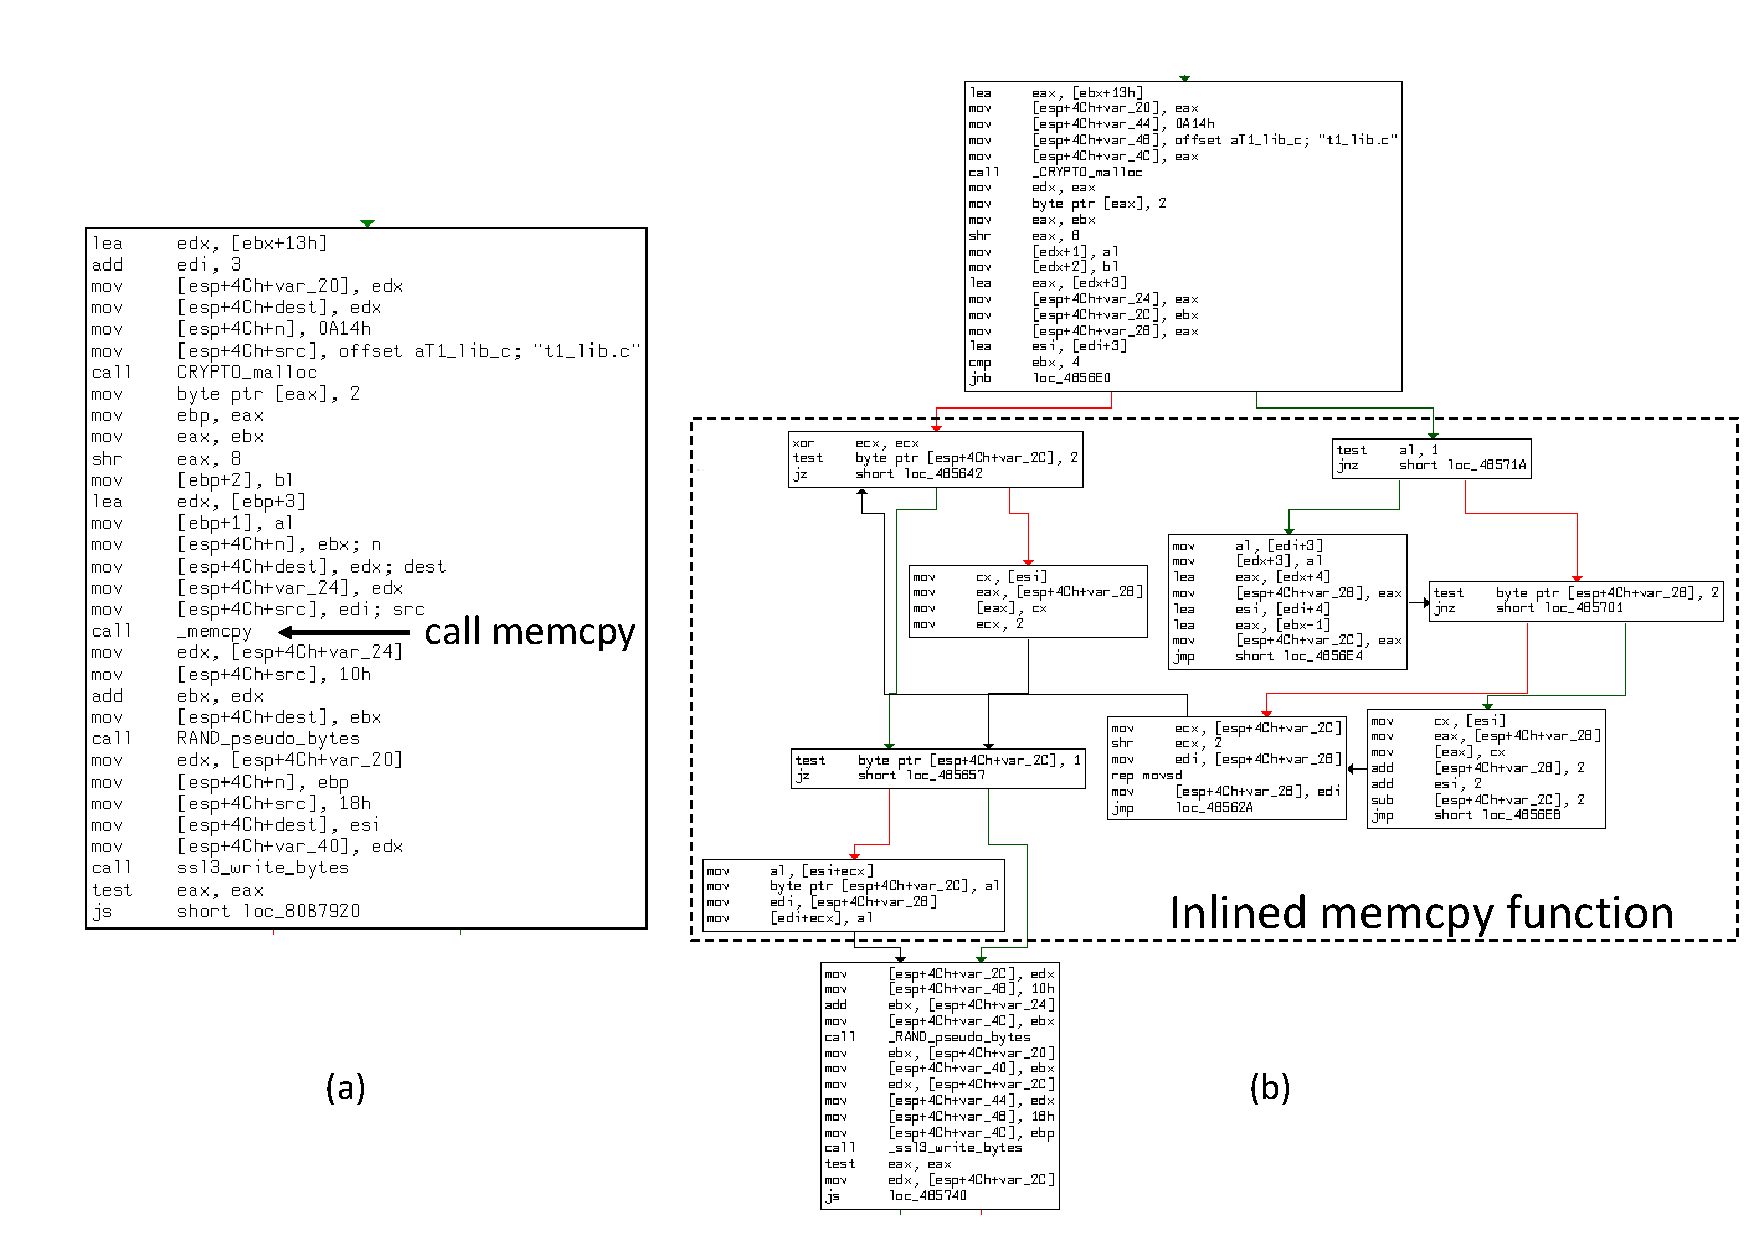
\includegraphics[width=\linewidth]{srj-figures/srj-moti_ex2.pdf}
  \caption{Code segment responsible for Heartbleed vulnerability (CVE-2014-0160) appeared as in the binary (a) compiled with \texttt{gcc} 4.6, and (b) compiled with \texttt{mingw}32} \label{fig:prob_stat}
% \vspace{-4mm}
\end{figure}


\begin{figure*}[th]
  \centering
  \subfigure[String copy via calling function \emph{strcpy}]{
    \label{fig:falseposi:a} %% label for first subfigure
    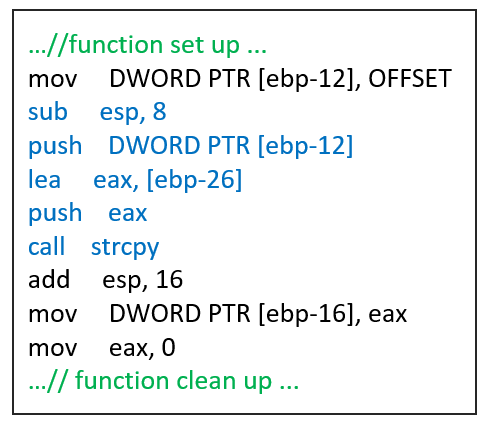
\includegraphics[width=1.8in]{srj-figures/bingoV_exam1a.png}}
  \hspace{1in}
  \subfigure[Memory copy in an iterative way]{
    \label{fig:falseposi:b} %% label for second subfigure
    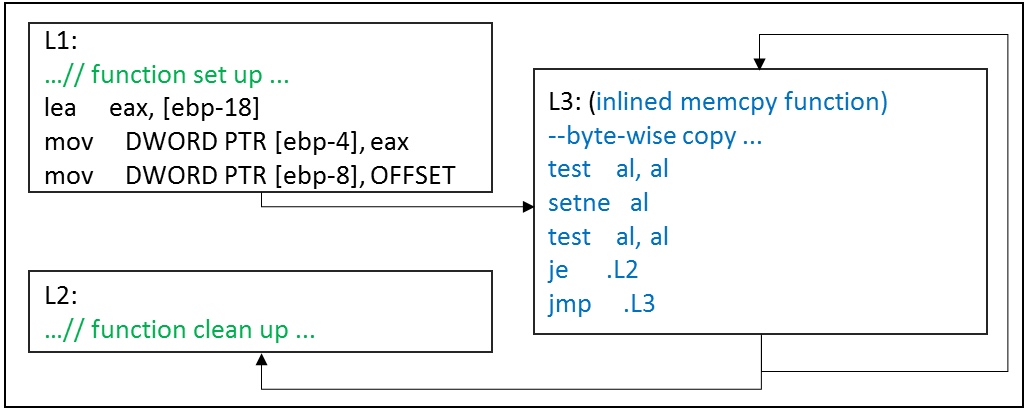
\includegraphics[width=3.82in]{srj-figures/bingoV_exam1b.png}}
  \caption{A false positive case of \tool}
  \label{fig:falseposi} %% label for entire figure
\end{figure*}

\section{Motivation} \label{sec:prob_state}
%Identifying semantically similar or equivalent binary code is a challenging task.
%In this section, %we discuss the problems of the existing binary code search techniques with motivating examples.
%Then
In this section, we state the challenges in the current research of cross-architecture and cross-OS binary code search  with illustrative examples. %We briefly introduce the solutions to these challenges, by leveraging selective inlining, combining different categories of features and adopting emulation.


 %for complete semantics analysis of functions and necessity to have a function model that is agnostic to underlying program structure.
%Then, we introduce the key challenges faced by existing binary function matching tools in detail.

%we \xyx{give a motivating example of binary matching regardless of architecture and OS differences, and state the challenges of  binary code search in finding the semantics and structures for this example. Last, we explain the basic idea of our proposed solution. }%and discuss their roles to achieve the scalable binary matching regardless of architecture and OS differences.}

\subsection{Motivating Example}  \label{subsec:bin_pre}

A binary program consists of a number of functions, each of which can be represented by the CFG (control-flow graph), a (directed) graph of basic blocks (BBs). The assembly instructions in a function are systematically  grouped into several BBs, which are considered as the building blocks of binary program. Thus, this BB-based representation is used by many static binary analysis tools.
%\begin{mydef}
%\emph{(\textbf{Basic-block}) A sequence of assembly instructions without any jumps or jump targets in the middle, where a jump target starts a block, and a jump ends a block.}
%\end{mydef}

%\begin{example}
 The same source code may produce binary code of different BB structures, due to different compilation configurations. Taking the heartbleed vulnerability (CVE-2014-0160) for example, Fig.~\ref{fig:prob_stat}(a) and (b) show the BB structures of the same source code compiled with \texttt{gcc} and \texttt{mingw}, respectively. Apparently, these two binary code segments share no identical BB structures --- with \texttt{gcc}, the vulnerable code is represented as a single basic block;  with \texttt{mingw}, represented as several basic blocks. A detailed inspection suggests that  library function \texttt{memcpy} is inlined in \texttt{mingw} version; while in \texttt{gcc}, it is not. %Due to this library function inlining, in \texttt{mingw}, the similarity between basic-blocks is affected considerably.
%Given the \texttt{gcc} version as a signature, we may miss the vulnerability in \texttt{mingw} version due to the function inlining.
Huge differences between the binaries in syntax and program structure make binary code search a challenging task.
%Hence, basic-block centric
%function modeling similarity matching(\textbf{P1}) and \mahin{program structure dependent pre-fitlering (\textbf{P3})} is not robust enough to address real-world problems. Further, this real-world scenario strongly suggest that functions should not be analysed in isolation, i.e., to capture the true semantics of a functions (\textit{caller}), all the related functions (\textit{callee}) also need to be taken in to consideration based on the caller-callee relationship (\textbf{P2}).
%\end{example}

 % and it is formally defined as follows (adapted from~\cite{david2014tracelet}):
%
%\begin{mydef}
%\emph{(\textbf{Type-k Partial Trace\footnote{In the rest of the sections, we'll use the term `partial trace' and `type-k partial trace' interchangeably, where `type-k partial trace' is used when referring to the length of a partial trace and in all other instances the term `partial trace` is used}}) Type-k partial traces is an ordered tuple of $k$ sequences, each representing one of the basic-blocks in a directed acyclic sub-path in the CFG, and containing all of the basic-block's assembly instructions.
%}
%\end{mydef}



%We introduce the term \emph{environment}, where binary is generated and executed, to denote the underlining architecture (e.g., Intel, ARM), the operating systems (OS) (e.g., Windows, Linux), the used compiler, and also the chosen compilation options.
%Different architectures have different instructions (a.k.a. ISA or Instruction Set Architecture) for the machine.
%Obviously, different environments will lead to considerably different binaries.

%\note{\textbf{I think we need make sure environment is used in the rest of the sections}}


%To better find the assembly code clones that perform similarly computational tasks, we formulate the concept of semantic clones.

% which has very important applications in both software security and software engineering. Despite the challenges, in the recent year, there are several good solutions proposed in academia to tackle this problem~\cite{pewnycross,ruttenberg2014identifying,egele2014blanket,luo2014semantics}. %of identifying semantically equivalent functions at binary level.
%However, none of the existing studies fills up the theory blank of \lq{}how a function is modelled\rq. %In the proposed modelling techniques of {\color{red}{using XXX}}~\cite{pewnycross,luo2014semantics}, it is assumed that basic-block structure is preserved across binaries, and thus, functions models should be  basic-block centric. Based on this assumption, semantic features are extracted from the sample functions at basic-block level and compared with the counterparts extracted from target functions in a pairwise way of basic-block comparison.


\subsection{Challenges for Syntactic Approaches}\label{sec:back:challenge}
Syntax is the most direct information usable for code search.
%However, the key challenge for syntax-based matching is:
%\noindent \textbf{C1: There is no consistent binary syntax representation across architectures.}
%Existing approaches mostly have attempted to use instruction patterns~\cite{DBLP:conf/uss/JangWB13,DBLP:conf/raid/KrugelKMRV05,saebjornsen2009detecting,DBLP:conf/pldi/DavidY14}, where for similarity matching, these approaches rely on syntax information. Though these techniques work well for the given environment (e.g., cases presented in~\cite{DBLP:conf/pldi/DavidY14}), it  fails for cross-architecture analysis, where syntax dramatically changes for different architectures~\cite{DBLP:conf/sp/PewnyGGRH15}.
%%For example, the two binary code segments in Fig. \ref{fig:idiom2-ex}, for ARM (left) and x86 32bit (right) architectures,  both represent the stack frame set up operation in function prologue.
%Hence, it is hard to perform similarity matching across architectures by purely relying on the syntax representation.
Most of existing approaches that rely on syntax information have attempted to use instruction patterns~\cite{DBLP:conf/uss/JangWB13,DBLP:conf/raid/KrugelKMRV05,saebjornsen2009detecting,DBLP:conf/pldi/DavidY14}.
As no consistent low-level syntax representation (i.e., assembly instructions) is available for cross-architecture search, these approaches fail for cross-architecture analysis. %\cite{DBLP:conf/sp/PewnyGGRH15} and CoP~\cite{luo2014semantics} use semantic features (e.g., symbolic expressions) and bug signatures to do cross-architecture analysis, respectively.}
To make binary code search across the architecture and OS boundary, semantics-based matching has been proposed~\cite{luo2014semantics,DBLP:conf/sp/PewnyGGRH15}, in which the machine state transition represents the semantics of a binary. Still, three challenges are faced in semantics-based matching.
%For example, the two binary code segments in Fig. \ref{fig:idiom2-ex}, for ARM (left) and x86 32bit (right) architectures,  both represent the stack frame set up operation in function prologue.

%\begin{figure}[ht]
%\small
% \centering
%  \begin{subfigure}[b]{0.5\linewidth}
%   % \includegraphics[width=0.75\linewidth]{srj-figures/srj-hierarchy-2.png}
%    \raggedright{\texttt{
%    \\
%    	mov ip, sp\\
%    	stm sp!, {fp,ip,lr,pc}\\
%    	sub fp, ip, 16\\
%    }}
%  %  \caption{\small{ARM version}}
%   \label{fig:idiom2-ex-a}
%    \vspace{1ex}
%  \end{subfigure}%%
%   \begin{subfigure}[b]{0.5\linewidth}
%   \centering
%   % \includegraphics[width=0.75\linewidth]{srj-figures/srj-hierarchy-2.png}
%    \raggedright{\texttt{
%    \\
%    	push ebp\\
%    	mov ebp,esp\\
%    	sub esp,16\\
%    }}
% %   \caption{\small{x86 32bit version}}
%   \label{fig:idiom2-ex-b}
%    \vspace{1ex}
%  \end{subfigure}%%
%  \caption{Function prologue for ARM (left) and x86 32bit (right)}
%  \label{fig:idiom2-ex}
%\end{figure}

\subsection{Challenges for Semantics-based Matching} \label{subsec:sem_chall}



\noindent\textbf{C1: The trade-off challenge of deciding the granularity of function model.} %: breaking the limits of basic-block structure.}
The state-of-the-art tools~\textsc{CoP}~\cite{luo2014semantics} and bug search \cite{DBLP:conf/sp/PewnyGGRH15} assume that BB-structure is preserved across binaries, and \xyx{a single BB can be matched with other BBs of similar semantics}. Based on BB-structure, semantic features are extracted and built into the function model. However, as admitted by Pewny \emph{et al.}~\cite{DBLP:conf/sp/PewnyGGRH15}, this approach is too sensitive to BB-structure differences, and hence problematic for smaller functions whose CFG structures are more susceptible to compilation options.
%Based on this, semantic features extracted from the signature function at basic-block level are compared with the counterparts extracted from target functions in a pairwise way.
%\emph{"Our metric is sensitive to the CFG and the segmentation of the basic block, which we found to be potentially problematic especially for smaller functions."}
%In practise, the assumption is too restrictive to be applied for real-world cases.
For example, the BB-structure compiled with  \texttt{gcc} 4.6 in  Fig.~\ref{fig:prob_stat}(a) is significantly different from that compiled with \texttt{mingw}32 in Fig.~\ref{fig:prob_stat}(b). In this case, the approach of BB-centric matching fails as no two BBs can match in Fig.~\ref{fig:prob_stat}.        % semantic features extracted from a single BB in these two cases will not contain the same semantics.





\noindent\textbf{C2. The accuracy challenge of using low-level semantic features.} %: covering the high-level and complete function semantics.}
Functions are considered in isolation by most of static tools, i.e., semantics of callee functions are not considered as part of the caller's semantics. This leads to partial semantics problem, especially when some common utility functions are implemented by the developers themselves (e.g., Adobe Reader has its own \texttt{malloc} implementation).
%Some existing techniques~\cite{wang2015binary} has noticed	the problem of basic-block, and propose to
\textit{Blindly inlining}  all the callee functions can be a remedy, as  all the user-defined functions are inlined in~\cite{wang2015binary}. %The blindly inlining strategy would lead to such a problem of code size explosion that the bloated functions are hard to analyze, incurring heavy overhead.
%However, one might assume that inlining all the callee functions at their respective call sites, as in~\cite{wang2015binary}, would solve the partial (or incomplete) semantics problem present in existing binary function matching techniques.
 Nevertheless, this approach fails in practice due to two main reasons: (1) heavy inlining may lead to code size explosion~\cite{chang1992profile},  %where performing similarity matching on bloated functions incur heavy overhead and hence,
and (2) not all the callee functions are semantically relevant to the caller function. %hence, inlining such functions might dilute the core functionality of the caller function, which in return, leads to poor matching results.
Thus, an inlining strategy is needed to decide that: \texttt{memcpy} should be inlined in Fig.~\ref{fig:prob_stat}(a) for matching with the semantically relevant one in Fig.~\ref{fig:prob_stat}(b). On the other side, \xyx{for functions not to be inlined, e.g., \texttt{ss13\_write\_bytes} in Fig.~\ref{fig:prob_stat}(a), features of library call information should not be ignored.}


\noindent\textbf{C3. The performance challenge of using static symbolic analysis or dynamic execution.} %: replacing with by micro execution.}
 Syntax based techniques, in general, are scalable~\cite{DBLP:conf/pldi/DavidY14}. As discussed earlier, they fail on cross-architecture analysis. To address this problem, semantics based approaches are preferred. However, extracting and solving low-level semantic features is a time-consuming job. Previously, we adopted an \emph{efficient} and architecture-, OS- and compiler-\emph{neutral} function filtering mechanism in \cite{bingo}. \xyx{With such mechanism, extracting input/output values of registers and flags of a function via constraint solving still takes 4,469s on average to extract low-level semantic features from 2,611 Linux \texttt{libc} functions --- it takes 1.7s to extract semantic features from a \texttt{libc} function. Hence, this part still has much space for improvement. To scale up code search for large-size binaries in real world, an efficient method is desired.}

\xyx{Previously, \tool has adopted $k$-tracelet for C1, selective inlining for C2, and filtering mechanism for C3 \cite{bingo}. However, \tool still suffers issues of false positive cases (see Fig.~\ref{fig:falseposi} and \S\ref{subsec:sem_chall_sol}) and inefficient feature extraction. In this paper, \toolNew adopts new features and emulation to address these issues (see \S\ref{sec:category}).}

%Therefore, to facilitate scalable semantic matching, an \emph{efficient}, and architecture, OS and compiler \emph{neutral} function filtering step is required.
%However, exiting approaches focus only on the efficiency aspect of the filter. For example, in~\cite{sebastian2016discovre}, only program structural features, such as number of basic blocks, are used as filters to speed up. However, as shown in Fig.~\ref{fig:prob_stat}, such features are not robust enough for cross-architecture, OS and compiler analysis.

%For example, due to the simplicity of the code in Fig.~\ref{fig:prob_stat}(a), there are many semantically irrelevant functions, which have the same number of basic blocks (i.e., one), to be filtered out before semantic matching.

%
%\noindent\textbf{C2: Semantics of binary code is too low level.}
%Due to the lack of explicit program semantics at binary level, machine state transitions of two totally unrelated code segments may look very similar (or identical), if the number of instructions in those binary segments are too small, e.g., the two code segments in Fig.~\ref{fig:code_seg}.
%A binary modeling approach based on machine state transitions has the problem of producing high false positives, especially when the given function (or vulnerability) signature is too small~\cite{DBLP:conf/sp/PewnyGGRH15}.
%%\ly{combine fig 2 and 3?}
%%Unfortunately, signatures, especially vulnerability signatures, having few instructions is common in real-world scenarios~
%
%\begin{figure}[t]
% \begin{center}
% \subfigure[A code segment to XX]{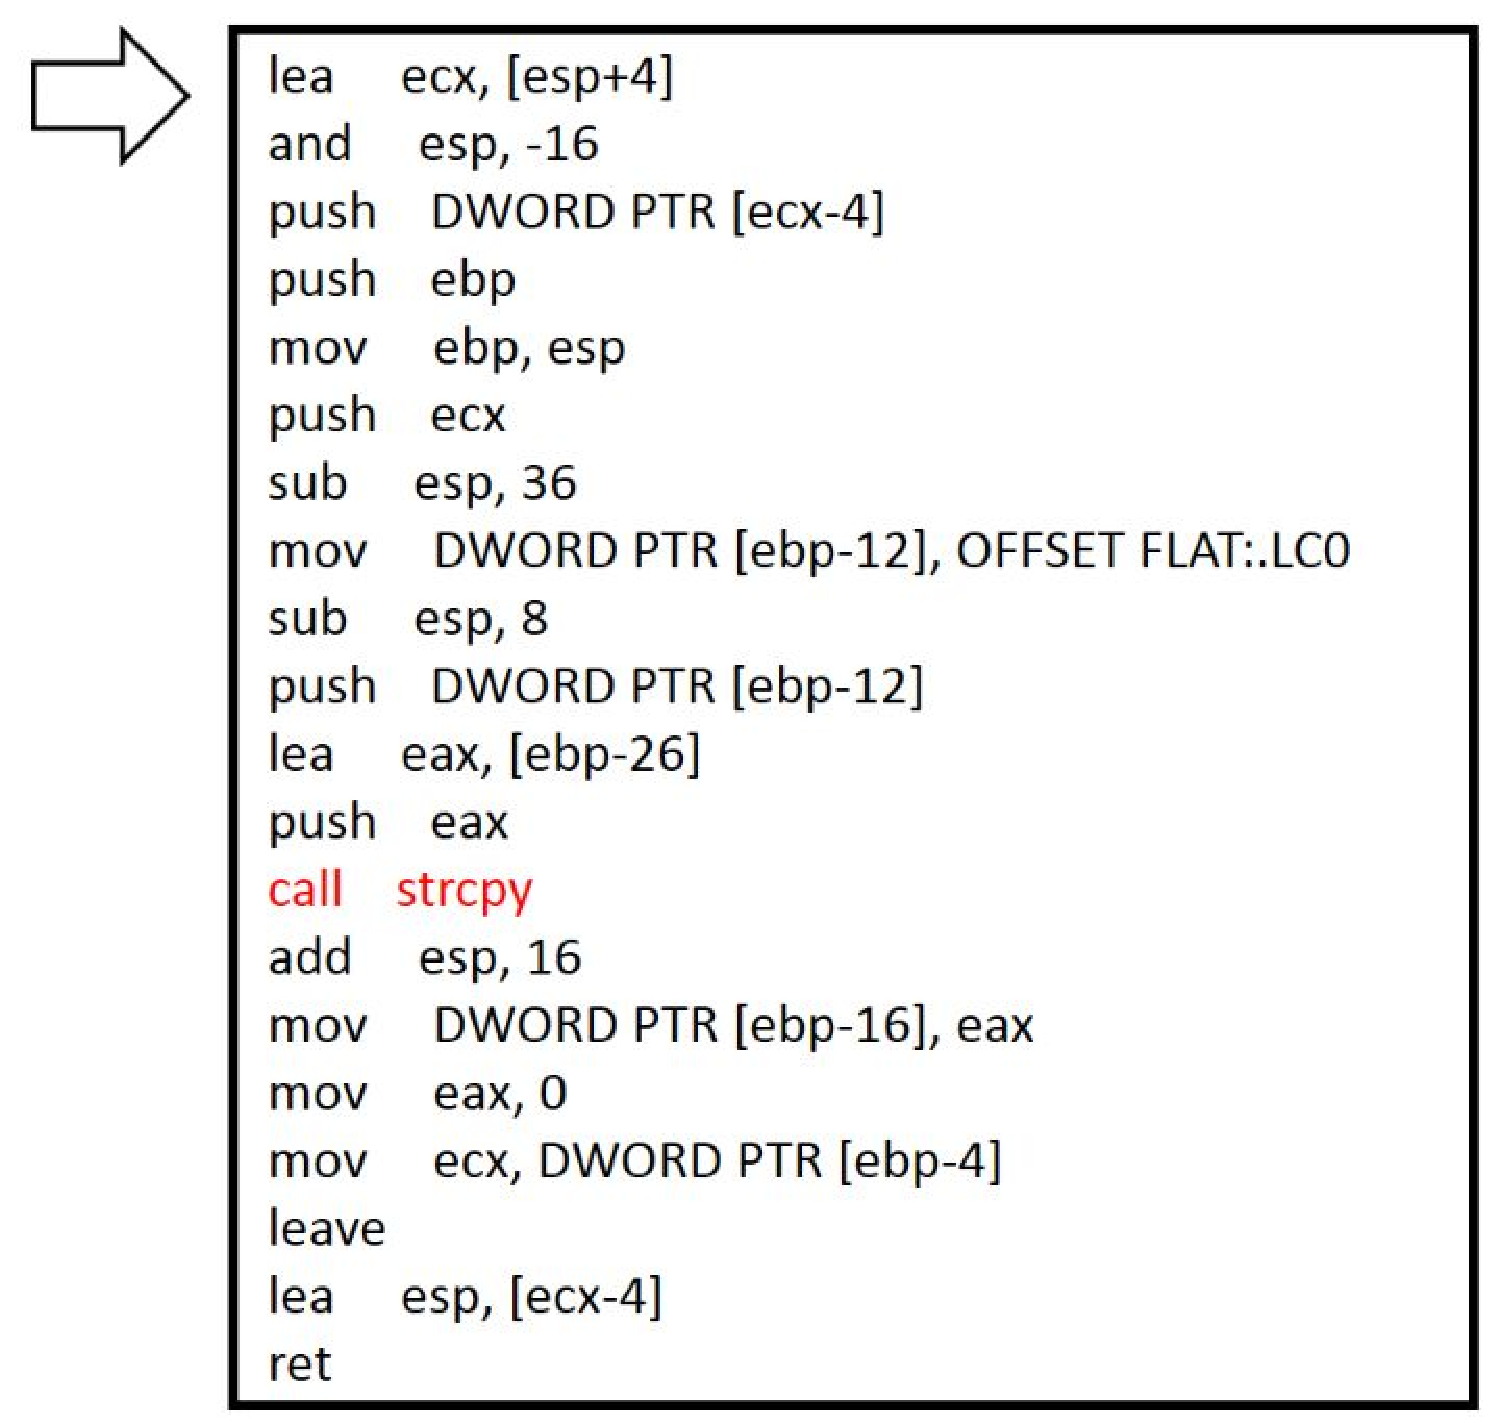
\includegraphics[width=200pt]{srj-figures/runexample1.pdf}}\label{fig:seg1:a}
% \subfigure[A code segment to XX]{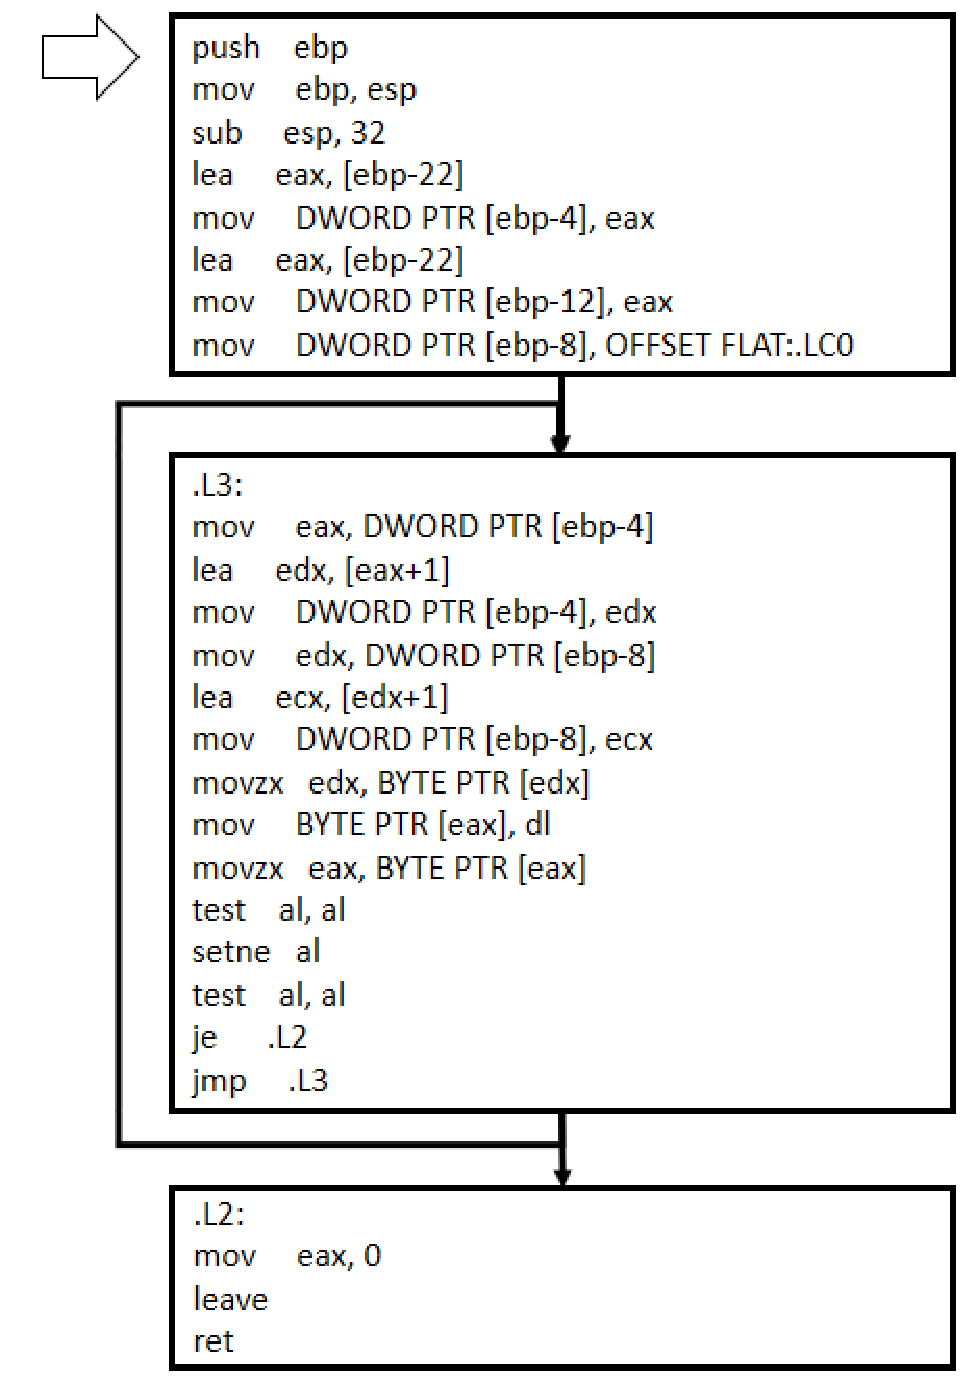
\includegraphics[width=200pt]{srj-figures/runexample2.pdf}}\label{fig:seg1:b}
%\end{center}
%\vspace{-4mm}
%\caption{\toolNew system architecture}
%\label{fig:code_seg}
%
%\end{figure}

%
%As shown in Fig. \ref{fig:state_seg}, two unrelated segments in Fig.~\ref{fig:code_seg} have the same initial machine state (i.e., pre-state) and also the identical post-state after execution. %, both code segments will result in .
%Here, code segment 1 adds the values in $\mathtt{EAX}$ and $\mathtt{EBX}$ registers, and move the results to $\mathtt{EAX}$ register. Since the pre-state values are all set to zero, after execution, $\mathtt{EAX}$ register will hold the value 0 and the condition-code flag $\mathtt{ZF}$ (zero flag) will be set to 1, since the result of addition operation is zero. On the other hand, in code segment 2, the value in $\mathtt{EBX}$ register is pushed to the stack, system API $\mathtt{strlen}$ is invoked, and finally the return value that is stored in $\mathtt{EAX}$ register is compared with an immediate value `0'. After execution, similar to code segment 1, $\mathtt{EAX}$ register will hold the value 1 as $\mathtt{strlen}$ system API is not interpreted (e.g., \cite{DBLP:conf/sp/PewnyGGRH15,luo2014semantics}), $\mathtt{EAX}$ register will hold the pre-state value, which is 0. In addition, the comparison operation will set the $\mathtt{ZF}$ to 1. In both executions, none of the other registers, condition-code flags and memory locations will be modified, hence retaining the pre-state values. From the examples shown in Fig.~\ref{fig:code_seg} and~\ref{fig:state_seg}, it can be seen that machine state transitions alone are not sufficient to model binary code.
%%\end{example}

%\noindent \textbf{C3: Computing the precise semantics is difficult and expensive.}
%Static methods~\cite{luo2014semantics,DBLP:conf/sp/PewnyGGRH15} using state-based semantic computation cannot capture the precise semantics due to missing the consideration of system APIs in the analysis.
%Dynamic analysis based techniques such as~\cite{egele2014blanket} might be able to address this problem. However, it is not scalable enough to handle large binaries. For example, in \cite{egele2014blanket}, before each function is executed, an environment needs to be set so that the execution does not terminate due to uninitialised memory handling. Unfortunately, considering the fact that a moderate size binary would easily have several thousand functions, this approach is not very scalable. %Hence, to address these challenges, we propose a partial traces based function modelling technique.







%\begin{mydef} \label{def:tracelet}
%\emph{\textbf{A partial trace} is \note{an instruction sequence obtained from basic-blocks that lie adjacent to each other along a program execution path. Partial traces can be of different length, where partial trace of length $k$ (called, Length-$k$ partial trace) denotes a partial trace that contains the instructions obtained from $k$ adjacent basic-blocks that lie along a program execution pat }}
%\end{mydef}
%
%\begin{mydef} \label{def:comp_semantic}
%\emph{\xyx{\textbf{Complete (or true) Semantics} refer to the contextual semantics that the function under analysis and %why we need true semantics of a function because compiler inline/outline certain functions
%}}
%\end{mydef}


%As discussed in Section \ref{sec:prob_state},
%The existing static binary function matching techniques, in general, fail to take into account the true (or complete) semantics of the functions under investigation. That is, each function in a binary is analyzed in isolation, where the semantics of the callee functions (be it user-defined or library function) are not considered when generating the caller function semantics as they are assumed to be two different functions. However, this assumption is intuitive and valid until we understand the caller-callee relationship (or dependency). For example, assume a user-defined function that manipulates string literals invokes the \texttt{strcpy} library function, and in order to capture the true semantics of the caller, it is \note{essential?} to inline \texttt{strcpy} function at the call site, as the caller function is involved in string manipulation, where it leverages on utility fucntions, such as \texttt{strcpy}, provided by the C runtime library to simplyfy its operations, hence, the semantics of the utility functions need to be considered as part of the caller fucntion semantics. Similarly, in another occasion, the programmer might implement her own version of \texttt{strcpy} function with additional security properties (called, \texttt{strcpy\_secure}\footnote{It is worth noting that \texttt{strcpy} is one of the banned function calls by Microsoft and hence, its better to use more secure variants such as \texttt{strncpy\_s} and \texttt{strcpy\_s}~\cite{msbannedfunctioncalls}}) and invokes it from all the string manipulation functions that need a secure string copy operation, hence, to capture the true caller semantics, the user-defined \texttt{strcpy\_secure} function needs to be inlined at the call site.

%To this end, in this paper, we propose partial trace based function modelling to overcome the aforementioned limitation.

%\noindent\textbf{$3$-tracelet or $k$-tracelet?}  In \cite{DBLP:conf/pldi/DavidY14}, $3$-tracelet, a concatenation of 3 adjacent basic-blocks, is used for searching. \textcolor{red}{Why k-tracelet is better.}


%Semantic based vulnerability detection at binary code level is an active research area and a promising direction towards securing closed-source software programs. However, we find that there is a gap in existing work \cite{pewnycross}\cite{ruttenberg2014identifying}, especially in vulnerability modelling, that is worth exploring. In the proposed vulnerability modelling techniques, it is assumed that basic-block structure is preserved across binaries \cite{pewnycross}, and thus, vulnerabilities are modelled basic-block centric. That is, semantic features are extract for from the basic-blocks in the known vulnerable function and they are compared with the basic-blocks in the target functions to identify the staring points of potential vulnerabilities.

%In \cite{ruttenberg2014identifying}, it is reported that for each basic-block in the signature (called, \textit{starting points}), first 20 basic-blocks (in-terms of similarity), in the target program, are selected for further signature matching. Similarly, in \cite{pewnycross}, for each basic-block in the signature, first 200 candidate basic-blocks, in the target program, are selected for the next level of vulnerability signature matching, using a greedy BHB (Best-Hit Boarding) algorithm. The commonality between these approaches is that the starting points, for vulnerability signature matching, are selected based on the similarity between basic-blocks in signature and target programs. However, the major drawback in this approach is that the basic-block structures can be easily distorted by factors that are beyond the control of security analysts.

%For example, figure \ref{fig:prob_stat}(a) shows the well-known heartbleed vulnerability (CVE-2014-0160) that shook the entire software industry. Figure \ref{fig:prob_stat}(a) shows the vulnerability at binary code level, compiled with GCC-4.6 and (c) shows the same vulnerability, but compiled with MinGW32. Immediately, we can say that the two programs doesn't share same basic-block structure. That is, with GCC, the vulnerable code is represented as a single basic-block, however, with MinGW, it is split into several basic-blocks. A deeper inspection would suggest that in MinGW version the library function \texttt{memcpy} is inlined while in GCC, it is not. Due to this library function inlining, in MinGW, the similarity between basic-blocks is affected considerably. That is, given the GCC version as a signature, we may miss the vulnerability in MinGW version due to basic-block \textit{splitting} and \textit{vice-versa} due to basic-block \textit{merging}. Hence, basic-block centric vulnerably modelling may not be robust against factors such as compiler type (version), optimization level and even difference in build environments. Therefore, in this paper, we present a more robust, self-adoptable vulnerability modelling technique.

%\todo {\color{blue} Do I need to include scope here? like doesn't not consider obfuscated binary that are hard to disassemble and only consider clean binaries without any obfuscations/packing.}

%\subsection{Problem Statement and Possible Solution} \label{subsec:pos_sol}
%To compare binaries, we need to define the criteria to compute similarity.
%In this work, we propose two complementary criteria to capture the semantic and structural information of the binary programs.
%Let $\mathcal{I}_1$ and $\mathcal{I}_2$ be two partial traces, we formally define the two kinds of similarity as follows:
%%The function $\langle\!\langle inst \rangle\!\rangle$ converts an instruction sequence (or an instruction) into a corresponding symbolic expression.
%
%
%\begin{mydef} \label{def:sem_sim}
%\emph{(\textbf{Semantic Similarity})
%Let $s_0$ denote a pre-state before executing $\mathcal{I}$, and $s_1=\langle\!\langle s_0, \mathcal{I}\rangle\!\rangle$ denote post-state after executing $\mathcal{I}$ on $s_0$. %post_\mathcal{I}^{pre_{\mathcal{I}}}=
%Let $S$ be set of all possible pre-states values that both $\mathcal{I}_1$ and $\mathcal{I}_2$ can execute on.
%The semantic similarity of $\mathcal{I}_1$ and $\mathcal{I}_2$, $SemSim(\mathcal{I}_1, \mathcal{I}_2)$, is defined as
%$\sum\nolimits_{s \in S} (\langle\!\langle s, \mathcal{I}_1\rangle\!\rangle -_m \langle\!\langle s, \mathcal{I}_2\rangle\!\rangle)$, where $-_m$ is a function to measure the difference of two machine states.
%%, the function $\langle\!\langle \bullet \rangle\!\rangle$ converts a partial trace into a set of \emph{symbolic expressions} and $\langle\!\langle \mathcal{I} \rangle\!\rangle(s)$ denotes assigning pre-state values $s$ to the symbolic expressions to yield the post-state values $ \mathcal{I}(s)$
%% are so \emph{similar in IO semantics} that they perform the similar computation tasks, if $PreS(\mathcal{I}_1)\approx reS(\mathcal{I}_2)$ and $PostS(\mathcal{I}_1)\approx PostS(\mathcal{I}_2)$.
%}
%\end{mydef}
%
%
%%In this work, a machine state is defined by the values stored at registers, condition-code flags and memory locations, which are common in all computing architectures.
%Semantic similarity is defined to capture the difference of the effects (i.e., post-state) of the binary program execution from the same input.
%Note that to calculate the precise effects of the program, we also need to consider the OS relevant information, like system API.
%Therefore, we consider that semantic similarity is architecture independent and OS dependent.
%
%%\ly{give one example of two code seg with different syntax, but same semantics}
%%Like example two in Fig. \ref{fig:state_seg}, the two code segments are not necessary to be from the same architecture, as the state model is not based on information that is architecture specific (see Section XX).
%
%Semantic similarity is one essential criteria to capture the behavior similarity of programs.
%However, this definition ignores the difference of program's structures, i.e., the program is treated as a black box.
%Due to the challenge \textbf{C2}, when comparing two binaries, we also want to consider the structures of the binary to make sure they are implementing the same algorithm or computation.
%%For example, bubble sort should not match with quick sort although they are semantically identical.
%This is critical in the tasks like code auditing, plagiarism detection and vulnerability detection.
%
%\begin{mydef} \label{def:comp_sim}
%\emph{(\textbf{Structural Similarity})
%The structural similarity of $\mathcal{I}_1$ and $\mathcal{I}_2$, $StrSim(\mathcal{I}_1, \mathcal{I}_2)$, is defined as
%$f^p_a(\mathcal{I}_1) -_f f^{p'}_{a'}(\mathcal{I}_2)$, where  $f^{p}_a(\mathcal{I}_1)$ (or $f^{p'}_{a'}(\mathcal{I}_2)$) is an abstraction function that maps $\mathcal{I}_1$ (or $\mathcal{I}_2$) to a structural model on architecture $a$, OS $p$ (or on architecture $a'$, OS $p'$); and $-_s$ is a function to measure the difference of two structural models.
%}
%\end{mydef}
%
%
%Structural similarity is a general definition. %, which aims to capture the high-level behavior of the binary code.
%The actual design of the abstraction function $f$ (e.g., using instruction patterns: $n$-gram~\cite{DBLP:conf/uss/JangWB13}, graphlet~\cite{DBLP:conf/raid/KrugelKMRV05} and tracelet~\cite{DBLP:conf/pldi/DavidY14}) reflects different research approaches on how to abstract the structural information of the binaries.
%Other usable structural information includes AST, PDG, data flow, type information and loop information.
%%For example, AST and PDG have been widely used for clone detection which reflect the syntax similarity.
%It is clear that the abstraction function is usually architecture and OS dependent, e.g., the codes in Fig.~\ref{fig:idiom2-ex}.
%%(e.g., using AST, PDG, data flow, type information, API and loop information)
%%Since the structureal information of assembly code (e.g., CFG) is usually architecture and OS specific, the direct matching based on CFG is not accurate, as shown in Fig. \ref{fig:prob_stat}. In this paper, we consider program information beyond the syntactic structure of the assembly code --- in addition, we also consider  data flow, type, API and loop information.
%
%%To capture the information relevant to semantics, we mainly consider data flow, API and partial traces in our model, while the structural information like BB is not the focus of our model.
%
%
%Overall, the similarity of $\mathcal{I}_1$ and $\mathcal{I}_2$ is defined as the combination of their semantic similarity and structural similarity.
%This similarity definition naturally resolves the challenge \textbf{C2}.
%
%To solve \textbf{C1}, we need to define a structural model, which is robust to different architectures and OSs. Motivated by the recent work on source code level idiom mining~\cite{allamanis2014mining},
%we propose to use the common binary patterns in different architectures and OSs as idioms, and use idioms to capture the program structural information, i.e., to define the abstraction function $f$.
%To support cross environments analysis, we propose a mapping of idioms in different architectures and OSs to a common concept such that $-_s$ can be easily computed.
%
%To solve \textbf{C3}, we propose a static analysis to capture the state-based semantics~\cite{DBLP:conf/sp/PewnyGGRH15} so that our approach is scalable.
%To capture the missing semantics related to system API using the static analysis, we introduce API idioms to complete the semantic information.
%Although the semantic comparison in this way is not precise as dynamic analysis like~\cite{egele2014blanket}, it works well with good scalability as shown in experiments.
%Furthermore, the idiom approach addresses the OS dependency problem in the semantic similarity definition.
%
%To solve \textbf{C4}, we propose a partial trace based function modeling, where partial traces of various lengths are extracted from binary code segment and they are organized in a systematic manner to handle program structure distortion. That is, by using partial trace models, no assumptions about the signature and target program structures are made (as in Tracy~\cite{DBLP:conf/pldi/DavidY14}).
%%However, in \tool, partial traces of varying lengths are considered, which doesn't make any assumption about the program structure}
%%By combining static analysis and feature hashing~\cite{jang2011bitshred}, our approach is scalable as no dynamic analysis is required.
%Overall, the unified idiom models for different environments make our solution work for all architectures and OSs.  The partial trace function modeling and complete semantic information give an accurate solution.
%
%
%%Different from \cite{allamanis2014mining}, the idiom mining is based on the tracelet from binary code and date dependency analysis. Our model is to capture the high level semantics of the assembly code, such as the idioms that abstract away the low level details, by which we search for the semantically similar assembly code regardless of architecture or OS differences,
%
%
%
%%In binary code similarity matching, due to the compilation process and optimizations, the syntax information is largely different.
%%
%% A desired model is needed to detect the assembly code in Fig \ref{fig:prob_stat} as similar, but the example in Fig \ref{fig:code_seg} not as similar. Hence, the model should be resistent to the syntactic differences due to BB structures, meanwhile, not encumbered by the issues of the pure similarly analysis of semantics. Hence, to strike a balance, we propose a partial trace (tracelet) based assembly code modeling technique.
%
%
%%To sum up, the computation model should leverages the static analysis for gaining the information from the three aspects: IO semantic based  model at the low level, tracelet based model at the middle level and idiom \cite{allamanis2014mining} based model at the high level.
%


\section{System Overview of \toolNew} \label{subsec:motivate_eg}

%Then, we explain the basic idea of our proposed solution and sketch the system overview.
%srj
%aum gaanathipathaye namaha
%\section{BinGo System Overview}\label{sec:overview}
%\note{not done - will do last after reviewing all other sections}
%compiler, architecture and OS agnostic
%\vspace{-3mm}
\begin{figure}[t]
\begin{center}
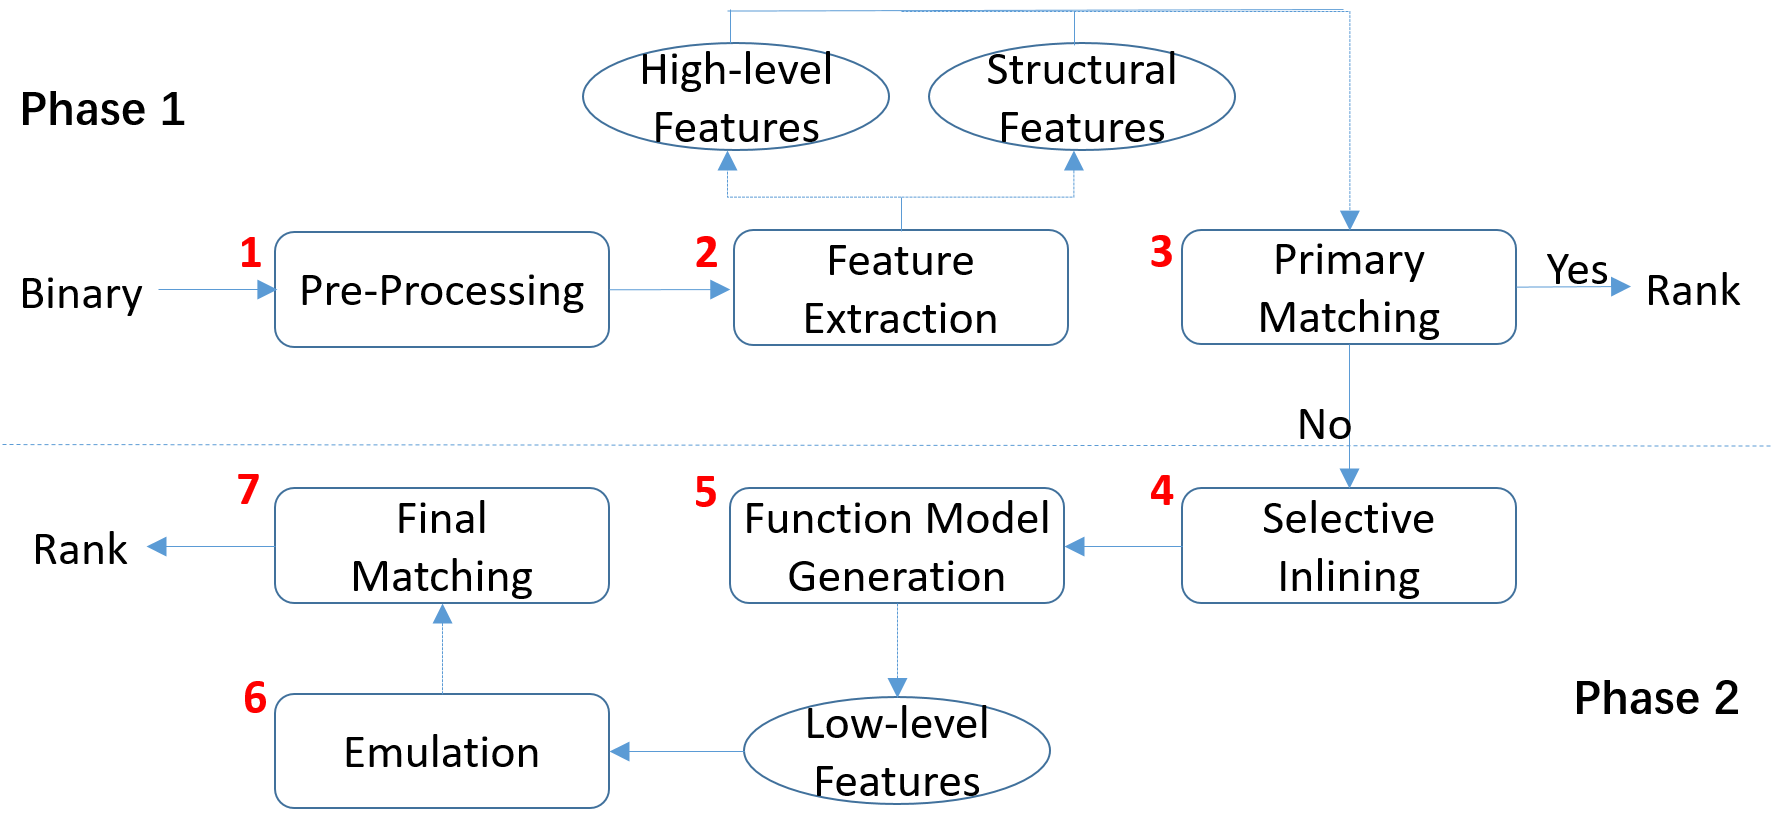
\includegraphics[width=9cm]{srj-figures/bingo_e_arch.png}
\caption{\toolNew work flow: rectangles represent processing steps, ovals represent features, arrows represent control/data flows}
\label{fig:archi}
\end{center}
\end{figure}

\toolNew, as a new extension of \tool, aims to be an accurate and scalable search engine for binary code. Given a binary function to be matched (\emph{signature function} in search), \toolNew returns the functions from the pool of analyzed binaries (\emph{target function} in search), ranked based on their semantic similarity.

\subsection{The Sketch of Work Flow} \label{subsec:workflow}
% Table generated by Excel2LaTeX from sheet 'Sheet1'

Fig.~\ref{fig:archi} shows the work flow of \toolNew. The input is one signature binary function and the possible candidate target functions. The output is the ranked list of candidate target functions above the user-defined threshold of similarity score. %, namely, pre-processing, selective inlining, filtering, partial trace generation, function model generation and similarity matching.
The basic idea is the two-phase matching: first employing the structural and high-level semantic features to find similar target functions;
if the similarity scores of all the returned target functions are below a certain threshold (\emph{No} flow after primary matching in Fig.~\ref{fig:archi}),  adopting the low-level semantic features to compare the I/O values on  $k$-tracelets of the signature function with those of candidate target functions.

We explain how each step in our approach works in brief. At step 1, given a signature function, it performs the preprocessing, i.e., disassembling  and building the CFG for the signature function.
At step 2, we extract these features from the high-level semantics and structure information in Table~\ref{tab:features}. \xyx{As shown in Table~\ref{tab:features}, we extract 6 types of high-level semantic features (\S\ref{sec:category:highSemanticFea}) and 3D-CFG structural features (\S\ref{sec:category:structralFea}).}
At step 3, \xyx{a primary matching step is conducted to measure the similarity  based on the Jaccard distance of high-level semantic features and the centroid distance of structural features (\S\ref{subsec:matching:primary})}.
If no results are above the similarity threshold, the process proceeds with comparing low-level semantic features (\S\ref{subsec:matching:lowFea}). At step 4, for each function in the target binaries, function calls are identified and selectively inlined according to the relevance of called libraries and other user-defined functions (\S\ref{sec:inline}). \xyx{Note that selective inlining is for addressing C2 (\S\ref{subsec:sem_chall}). Selective inlining is transitive. Assume function $a$ calls function $b$ and $b$ calls function $c$. If $a$ selectively inlines  $b$, then the decision of inlining $c$ into  $b$ is according to Algorithm \ref{algo:select-inline} (\S\ref{sec:inline}). If $a$ does not need to inline $b$, then it is certainly unnecessary to inline $c$ into  $b$.}
%Then from these inlined target functions, we shortlist a list of candidate functions that are similar to the signature function by using three filters, which consider different aspects of the binary semantic (\S\ref{sec:prefilter}). %, where at the end of filtering process, \tool returns a list of target functions that are similar to the signature function.
%It is noted that selective inlining (Section~\ref{sec:inline}) is carried out as part of filtering process.
At step 5, for the signature functions, length variant partial traces (up to $k$-tracelets) are generated  and grouped to form the function models (\S\ref{subsec:partial_trace_ext}), which  low-level semantic features are extracted from (\S\ref{subsec:fun_mod_mat}). %(\S\ref{subsec:sem_fea_ext}), and these features are later used for semantic similarity matching.
%Note that for candidate target functions, the process to function model generation, which just needs to be carried out for once, has been completed before.
Note that function model generation and feature extraction is a one-time job.
At step 6, we rely on emulation to get the input/output values, flags, memory addresses of signature functions as low-level semantic features (\S\ref{sec:emulation}).
Finally, at step 7, combining \xyx{Jaccard Distance} for low-level semantic features and results of the primary matching, \toolNew returns target functions that are above the similarity threshold in a ranked order (\S\ref{subsec:matching:final}). %, where rank \#1 is the \xyx{best} match to the signature function.

%The structure of following sections is:
The approach is presented in the following way: in \S\ref{sec:category}, different categories of features and emulation (step 2 and 6) are introduced; in \S\ref{sec:inline}, selective inlining (step 4) is elaborated; in \S\ref{sec:func_match}, the key steps 3, 5 and 7 are explained with details. %\S\ref{sec:experiemntation} presents evaluation results; \S\ref{sec:related} reviews the literatures; and \S\ref{sec:concl} concludes the paper.

%\tool will generate funIt is noted that to selective inlining is performed on all the target fucntions to extract


%\mahin{I didn't explain each of the modules here, either we can bring section 2.4 (proposed solution) here, or move this to sec 2.4 }

% and post-processing module.
%Given a binary program, \tool will first dissemble it into REIL intermediate representation (REIL IR).
%
%In the feature extraction module, two types of semantic features are extracted from partial execution traces: semantic features and structural features. State-base semantic features (see Section~\ref{subsec:stat_sem}) represent the low-level effects of executing the binary code in terms of machine state (i.e., characterised by register, condition-code flag and memory values) at various program points.
%Semantic features of API idioms (see Section~\ref{sec:idiom:def}) capture the OS dependent semantics of the binary code.
%Secondly, structural features and compiler idioms (see Section~\ref{sec:idiom:def}) can help to quickly find the binary code with similar program structural or representations.
%These features complementarily summarize the behaviour of binary code at various granularity levels, providing a comprehensive view to overcome the differences at syntax and structural levels. This is the one of the key contributions of this work for achieving accurate yet robust matching results.
%%In generating partial execution traces, we employ a \textit{pruning} technique that removes infeasible executions soundly, with the help of a theorem prover.
%
%In the function model generation module, for each function, a number of \textit{function models} are generated based on different combinations of partial traces.  Specifically, partial execution traces of various lengths are combined in different ways to represent the function models that account for structural changes in the compiled code, such as function inlining and outlining introduced by the compilers. For a given function, if partial traces of $n$ different lengths are generated, the function can be represented by $2^n-1$ different function models.
%
%Finally, the machine learning module applies feature hashing techniques on functions models, generated from each function, where they are put into `bins' based on their proximity to each other. That is, function models that are similar, in terms of syntax and semantic features, will likely to get into the same bin. Hence, for a given search query, using feature hashing, the appropriate bin is located and the matching functions are obtained from there. This improves searching time.

%Finally, post-processing module removes the outliers and variants of the same function in the search results, to improve the overall search ranking. For example, given two variants of the same function (e.g., \texttt{strncpy\_ia32} and \texttt{strncpy\_sse}) in the search results (e.g., assume \texttt{strncpy\_ia32} is ranked 1 and \texttt{strncpy\_sse} is ranked 2), only the highest ranking function (\texttt{strncpy\_ia32}) is kept in the search results and others are removed from it.


%In the following sections, we shall discuss the four modules in details.
%In practise, security analysts get to know about new vulnerabilities from a patch or a CVE advisory and, using the features (or characteristics) extracted from the known vulnerability (called, \textit{signatures}), try to find similar vulnerabilities in the programs they are interested in or concern about (called, \textit{target programs}).

%As can be seen in figure \ref{fig:overview}, our system consists of two phases, a pre-processing phase and a vulnerability signature matching phase. In preprocessing phase, we pre-process the program binaries for our vulnerability signature matching. In this phases, we first, disassemble the binary program and extract the control-flow structures. Then, synthetic features (i.e., code properties) are extracted from the disassembled functions. Next, each function is modelled using \textit{tracelet models}, where tracelet (explained in section \ref{subsec:vul_mod}) is a sequence of $n$ adjacent basic-blocks. Finally, from each tracelet model, the semantic features are extracted. It is important to note that the pre-processing only has to happen once per signature and target program. The pre-processed output can be reused in the future, for new vulnerability searches.


%In the vulnerability signature matching phase, our system searches for a signature within a target program and identifies binary code parts which are similar to the vulnerability signature. First, we first quickly search the target binary, using the synthetic features (i.e., code properties), to identify candidate functions (i.e., potentially vulnerable) in the target program . This pre-filtering process is cheap in terms of computational cost and considerably improves the scalability, where it reduces the number of `potentially' vulnerable functions from several thousands to few hundreds (sometimes even smaller), in the target program. Next, we compare the signature program against the selected candidate target functions using semantic features extracted in the pre-processing phase. To this end, we use the \textit{symbolic expressions} (explained in section \ref{subsec:sem_fea}, at high-level, it represents the effect of a piece of code on the program-state), extracted from the signature tracelet models and compare them with the symbolic expressions, extracted from the target tracelet models.
%Here, it is worth mentioning that $k_s$ take a single value, i.e., we fix the length of the tracelet for vulnerability signature (e.g., $k_s=3$), whereas $k_t$ takes a range of values starting from $1$ upto $n$ ($k_t\in\mathbb Z_{> 0}$), i.e., for a given bug signature, we try to match tracelets of various lengths, in the target function,  and choose the tracelet that is close to the signature in-terms of semantic similarity.

%Here, it is worth mentioning that the length of tracelets, for both signature ($k^s$) and target ($k^t$) programs, takes a range of values starting from $1$ upto $n$, where $n\in\mathbb Z_{> 0}$. For example, given a signature tracelet of size 2 (i.e., $k^s=2$), we try to match tracelets of various lengths (e.g., $k_s=1,2,3$), in the target function, and choose the tracelet that is closest to the signature in-terms of semantic similarity (i.e., \textit{optimal} tracelet model). In this way, we introduce self-adaptability in modelling the vulnerability, which allows us overcome the challenges, such as vulnerability models being sensitive to basic-block \textit{splitting} and \textit{merging}, prevailed in the vulnerability modelling techniques reported in the literature \cite{pewnycross}\cite{ruttenberg2014identifying}. Finally, at the end of the workflow, our system reports the similarity matrix, revealing the optimal tracelet models (i.e., optimal values for $k^s$ and $k^t$) for signature and target programs that maximize the tracelet similarity. From this, we can identify the target functions that are similar to the vulnerability signature and the optimal tracelet models, for both signature and target programs, that better represent the vulnerability.
 %~\xyx{In step 5, to facilitate cross-architecture analysis, to address the syntax differences of instructions, we lift the low-level assembly instructions into a corresponding intermediate representation (IR) and extract low-level semantic features based on that.}
%To mitigate C1 (the single basic block matching to several basic block matching in Fig.~\ref{fig:prob_stat})), we borrow the idea of tracelet used in \textsc{\small Tracy}~\cite{DBLP:conf/pldi/DavidY14}. Different from the original approach that uses a fixed length of tracelet, we use length variant partial traces. %to mitigate the effect of program structure distortion especially basic block structure.
%Next, to overcome C2 (e.g., whether to inline \texttt{memcpy} in Fig.~\ref{fig:prob_stat}(a)), we propose a selective inlining strategy to strike a balance between the needed contextual semantics and the overheads due to inlining. Finally, to address C3, we adopt three filters considering different aspects of the semantics to identify the similar functions.


%\mahin{I feel, fast filtering in our FSE paper and high-level features in this paper are slightly over lapping. In filtering, we rely on API names and instruction types to filter the candidate target functions (we have 3 types of filtering in FSE paper). In 'high level' features mentioned in this paper, we have API names/sequence, instruction types, function parameter details, function local variable details. So, you can  see that filtering is a subset of high level features.  I am thinking, in this paper, in the filtering step, we can use high-level and structural features to filter the candidate function (these two features are very scalable and thus, can be used in the filtering step?) and use low level features (which is more expensive in-terms of performance cost) in the function model generation step?}
\begin{table}[t]
  \centering
  \caption{Different categories of features used by \toolNew}
    \begin{tabular}{|p{2.5cm}|p{2.5cm}|p{2.5cm}|}
    \hline
    \textbf{Low-level Semantic Feature} & \textbf{High-level Semantic Feature} & \textbf{Structural Feature}\\ %& \textbf{locality-based similarity} \\
    \hline
    \multicolumn{1}{|l|}{mem. operations} & op. type & \multicolumn{1}{l|}{BB sequence} \\ %& \multicolumn{1}{l}{inbound } \\
      flags    & system call tags & \multicolumn{1}{l|}{loop information}  \\ %& \multicolumn{1}{l}{outbound} \\
      registers    & function call seq. & \multicolumn{1}{l|}{In-degree of BB}  \\ %&  \\
          & function parameter & \multicolumn{1}{l|}{out-degree of BB}  \\ %&  \\
          & local variable &        \\ %&  \\
          & op. code &        \\ %&  \\
          \hline
    \end{tabular}%

  \label{tab:features}%
\end{table}%


\subsection{Solutions to the Matching Challenges} \label{subsec:sem_chall_sol}

Here, we highlight how \toolNew overcomes the challenges aforementioned in \S\ref{sec:back:challenge} and improves \tool.

\noindent\textbf{S1: \emph{Flexible function model} via $k$-tracelet and 3D-CFG.}
In \tool and \toolNew, to address C1, we borrow the idea of tracelet in \textsc{Tracy}~\cite{DBLP:conf/pldi/DavidY14}, where David \emph{et al.} extract  a fixed-length partial trace of 3 BBs (3-tracelet). Then they check semantic equivalence between 3-tracelets based on data-dependence analysis
and rewriting, in which constraining solving is applied to verify input/output invariants among the registers, flags and variables. In \tool, we use a set of variant-length partial traces (i.e., a set of $k$-tracelet, $k$ is up to 4) to represent the function model. In \toolNew, we complement the tracelet-based approach with function structural information (i.e., 3D-CFG). \xyx{3D-CFG is resilient to BB structure changes due to optimization levels, as it uses structural information of a function as a whole.}%, not like BB-based graph matching approaches}.

\noindent\textbf{S2: Completing function semantics via \emph{selective inlining} and identifying the \emph{high-level semantics.}}
To mitigate the issue of incomplete semantics of the analyzed function, selective inlining is proposed in \tool. However,  several FP cases are observed during semantic matching, where low-level
semantic features are insufficient to reveal the true functionality. \xyx{For instance, two code segments in Fig. \ref{fig:falseposi} cannot be distinguished by low-level semantic features as they have the same input and output results for any given string input. In fact, they have different functionalities, as the code in Fig. \ref{fig:falseposi}(a) copies the string array via calling function \emph{strcpy}, and the code in Fig. \ref{fig:falseposi}(b) does the memory copy (not limited to string copy) in an iterative way}. In \toolNew, we consider not only low-level semantic features (e.g., symbolic features on register, flag, memory status), but high-level semantic features that are relevant  to function calls, including system calls and library calls. %\xyx{Thus, selective inlining and high-level features are combined to achieve the complete and abstract function semantics.}

\noindent\textbf{S3: Efficient semantics extraction via binary code \emph{emulation}.}
\xyx{In order to speed up the process of extracting low-level semantic features, we propose to apply Unicorn \cite{unicorn} to virtually execute the extracted partial traces and identify the input/output values from them. Unicorn is a lightweight multi-platform, multi-architecture CPU emulator framework, which is built on QEMU. According to the manual \cite{unicorn}, for extracting low-level semantic features, emulation may boost the efficiency by one or two orders of magnitude, compared with constraint solving.}


To sum up, in Fig.~\ref{fig:archi}, step 2, 3, 6 and 7 are newly introduced into \toolNew. Among them, step 2 and 3 are the implementation of \textbf{S1} and \textbf{S2}, while step 6 is the implementation of \textbf{S3} (\S\ref{subsec:sem_chall_sol}). Note that in step 2, only the static analysis is required so that the process of feature extraction is scalable. In step 6, to avoid the overheads of actual execution or constraint solving for extracting low-level features, emulation is adopted to speed up the process. \xyx{In step 7, to remove the false positive cases due to matching with low-level semantic features alone, the results of step 2 (similarity in high-level semantics and BB-structure) are also considered (\S\ref{subsec:matching:final})}.

%\xyx{\textbf{UP\_TILL\_HERE}}

\section{Binary Code Matching Features}\label{sec:category}

In this section, we elaborate the features that we adopt to measure the similarity of two binary code segments.  As listed in Table \ref{tab:features}, these features fall into three categories. For each feature in Table \ref{tab:features}, the example and description are given in the following subsections. Features of structures and high-level semantics are extracted via static analysis, which is the functionality of step 2. Features of low-level semantics are extracted by emulation (step 6).


\subsection{Structural Features}\label{sec:category:structralFea}

3D-CFG~\cite{3d-cfg} depicts the CFG structure of a function at a high-abstraction level. It is used to measure the similarity between methods in/among bytecode of Android apps. The basic idea in \cite{3d-cfg} is to assign a structural 3D-coordinate value for each node in the control flow graph (CFG) of a method, then calculate the mass centroid of these coordinates as the centroid of the method. By calculating the distance between two methods' centroids, the similarity among these two methods can be measured.

According to \cite{3d-cfg}, for a given method, each node in the CFG is a basic code block. Each node has a unique coordinate, denoted as a 3-tuple $(x, y, z)$, where $x$ is its sequential number in the CFG; $y$ is the number of its outgoing edges (out-degree of the node in CFG), and $z$ is the loop depth of the node.

Based on the nodes inside the function $f$, we define the  centroid $\overrightarrow{c_f}$ of  function $f$:


\begin{mydef}\label{thm:cdd} The centroid is a 4-tuple $(c_{x}, c_{y}, c_{z}, w)$~\cite{3d-cfg}:
\begin{itemize}[itemsep=0.1mm]
  \item $w~=~\sum_{e(p,q)\in3D-CFG}(w_{p}+w_{q})$,
    \item $c_{i}~=~\frac{\sum_{e(p,q)\in3D-CFG} (w_{p}i_{p}+w_{q}i_{q})}{w}, where~i\in\{x,y,z\}$
\end{itemize}\vspace{-1mm}
\end{mydef}
\noindent where $e(p,q)$ is the edge between the node $p$ and $q$, $(x_{p}, y_{p}, z_{p})$ is the coordinate of the node $p$, and $w_{p}$ is the number of assembly instructions in the node of BB.

To emphasize the importance of function call instruction (relevant to high-level semantics), the weighted centroid is defined as $\overrightarrow{c_f}' = ({c}_{x}', {c}_{y}', {c}_{z}', w')$ for function $f$, where $w' = w + N$, and $N$ is the number of function call instructions; ${c}_{x}',~{c}_{y}'$ and ${c}_{z}'$ are recalculated according to the new weight $w'$, respectively. Suppose each BB node in Fig.~\ref{fig:strucFea} contains only one instruction ($w_A=1, w_B=1, w_D=1$), and node $C$ contains one function call instruction  ($w_C=2$). We have the following coordinates: $(1,2,1)$ for $A$, $(2,2,1)$ for $B$, $(3,1,0)$ for $C$ and $(4,0,0)$ for $D$. Then, the centroid is \xyx{$(2.2,1.5,0.6,10)$} and the weighted centroid is \xyx{$(2.38,1.38,0.46,13)$}. %(where $w=10$, $N=1$ and $w'=13$).
%For example, for the first method in Fig.~\ref{fig:motivation}(a), the centroid is $(1,0,0,5)$ and the weighted centroid is $(1,0,0,9)$ (only four invocation statements). Note that $w'$ is 9, the sum of $w$  and the number of invocation statements.

Given a function $f$, the function signature $\overrightarrow{f} =(\overrightarrow{c_f}, \overrightarrow{c_f}')$ is a feature vector containing the structural  information of the function, where  $\overrightarrow{c_f}$ is the centroid, $\overrightarrow{c_f}'$ is the weighted centroid.

The difference between the centroids of two functions $f_1$ and $f_2$ is the primary condition to evaluate their similarity:
 
\begin{mydef}\label{thm:cdd}
The Centroid Difference Degree (CDD)~\cite{3d-cfg} of two centroids $\overrightarrow{c_1} =({c_1}_{x}, {c_1}_{y}, {c_1}_{z}, w_1)$, $\overrightarrow{c_2}=({c_2}_{x}, {c_2}_{y}, {c_2}_{z}, w_2)$
(the distance of the weighted centroids  $\overrightarrow{c_1}'$ and $\overrightarrow{c_2}'$) is
 
\begin{small}
\begin{center}
$
CDD(\overrightarrow{c_1}, \overrightarrow{c_2}) = max(\frac{|{c_1}_x-{c_2}_x|}{{c_1}_x+{c_2}_x}, \frac{|{c_1}_y-{c_2}_y|}{{c_1}_y+{c_2}_y},\frac{|{c_1}_z-{c_2}_z|}{{c_1}_z+{c_2}_z},\frac{|w_1-w_2|}{w_1+w_2}) \nonumber
$
\end{center}
\end{small}
\end{mydef}

Given two functions, the function-level difference degree is defined as the maximum value between their centroid distance (CDD) and their weight centroid distance (weighted CDD):

\begin{mydef}
Function Difference Degree (FDD) of two functions $\overrightarrow{f_{1}}=(\overrightarrow{c_{1}}, \overrightarrow{c_{1}}' )$ and $\overrightarrow{f_{2}}=(\overrightarrow{c_{2}}, \overrightarrow{c_{2}}' )$ is
{
\begin{small}
\begin{center}

$FDD(\overrightarrow{f_{1}}, \overrightarrow{f_{2}}) = max(CDD(\overrightarrow{c_{1}}, \overrightarrow{c_{2}}),CDD(\overrightarrow{c_{1}}', \overrightarrow{c_{2}}'))$
\end{center}
\end{small}
}
\end{mydef}

\begin{figure}[tb]
\begin{minipage}{0.5\linewidth}
\centering
\scriptsize
 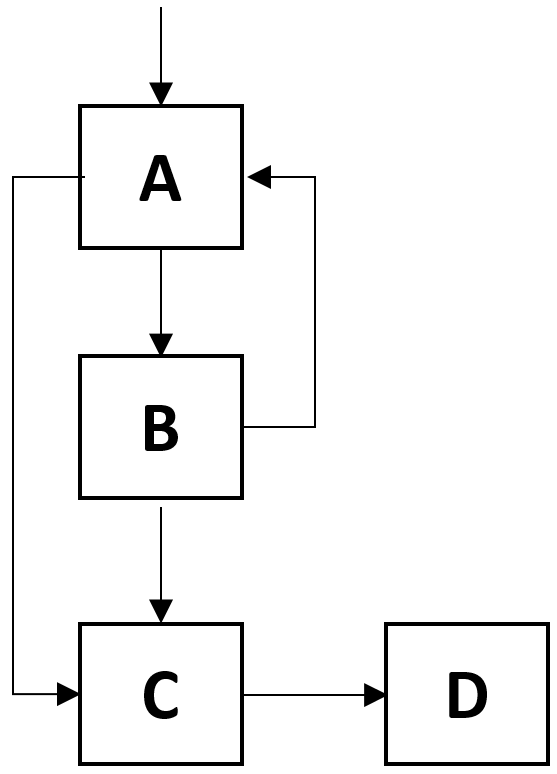
\includegraphics[width=2 cm]{srj-figures/3d-cfg.png}
%\\[0.2cm] (a) candidate DFA $\mathcal{C}_1$
\end{minipage}
~
\begin{minipage}{0.5\linewidth}
\centering
\scriptsize
\begin{tabular}{l} \hline
\textbf{Structural features:} \\
BB sequence: \\
~~~~main: $A \to B \to C \to D$ \\
~~~~the sequential number of BB (A): $1$ \\
In-degree of BB (A): $2$ \\
out-degree of BB (A): $2$ \\
Loop information: \\
~~~~The loop depth of BB (A): $1$ \\
~~~~involving number of BBs: $2$ \\
\hline
\end{tabular}
%\\[0.2cm] (b) candidate DFA $\mathcal{C}_2$
\end{minipage}
\vspace{-2mm}
\caption{The BB-structure of a function, and its structural features
}
\label{fig:strucFea}
\end{figure}

The two code segments in Fig.~\ref{fig:falseposi} will not be matched as similar according to these structural features. \xyx{Since the code segment in Fig.~\ref{fig:falseposi:a} has only one BB and the code segment in Fig.~\ref{fig:falseposi:b} has 3 BBs. Their CDD and weighted CDD are all 1 ($c_{1y}$ and $c_{1z}$ are all 0), which indicates zero similarity  according to~\cite{3d-cfg}\cite{DBLP:conf/issta/MengXXLZN16}.  Thus, 3D-CFG captures the overall structure of a binary function; and it is effective in measuring the structural similarity of two given binary functions.}

 \subsection{High-level Semantic Features}\label{sec:category:highSemanticFea}
For the high-level semantics, we mainly make use of the operation types, system call tags (tags of function calls to system APIs), function call sequences, function call parameters, local variables and op. code.  The basic idea is that  function calls (especially system calls) carry the semantics of code and they can be used for semantic-based code matching tasks,  e.g., system-call based malware detection~\cite{DBLP:conf/issta/CanaliLBKCK12}. Hence, the information of function calls (tags, parameters, sequences) is extracted as features. Additionally, we extract features from the numbers of different types of binary instructions. \xyx{We first classify different binary instructions into 15 categories\footnote{The instructions inside each category can be found from this link: \url{https://sites.google.com/site/toolbingoe/instruction-category}}, including \emph{data\_transfer}, \emph{arithmetic}, \emph{stack}, \emph{logical}, \emph{shift\_rotate}, \emph{control\_transfer}, \emph{loop}, \emph{string}, \emph{flag}, \emph{misc}, \emph{sign}, \emph{fstp}, \emph{port}, \emph{mmx}, \emph{call}.
Then we use the number of instructions in each category as a feature.} Last, we also extract features from local variables. The reason is that  local variables may represent the intermediate values in the execution, and the same intermediate values indicate the same or similar function semantics.




\begin{figure}[tb]
\begin{minipage}{0.5\linewidth}
\centering
\scriptsize
 \begin{tabular}{|l|}  \hline
$\mathtt{push \quad    ebp}$\\
$\mathtt{mov  \quad ebp, esp}$\\
$\mathtt{sub  \quad esp, 56}$\\
$\mathtt{sub  \quad esp, 8}$\\
$\mathtt{lea  \quad  eax, [ebp-16]}$\\
$\mathtt{push \quad   eax}$\\
$\mathtt{push \quad   OFFSET~FLAT:.LC0}$\\
$\mathtt{call \quad   scanf}$\\
$\mathtt{add  \quad    esp, 16}$\\
$\mathtt{mov  \quad    eax, DWORD~PTR [ebp-16]}$\\
$\mathtt{sub  \quad    esp, 12}$\\
$\mathtt{push \quad   eax}$\\
$\mathtt{call \quad   strlen}$\\
$\mathtt{add  \quad    esp, 16}$\\
$\mathtt{mov  \quad    DWORD~PTR [ebp-12], eax}$\\
$\mathtt{cmp  \quad    DWORD~PTR [ebp-12], 9}$\\
$\mathtt{jg   \quad    .L2}$\\
 \hline
\end{tabular}
\\[0.2cm] (a) basic block $B_1$\\
 \vspace{2mm}
 \begin{tabular}{|l|}
  \hline
$\mathtt{ mov \quad  eax, 0 }$~~~~~~~~~~~~~~~~~~~~~~~~~~~~~~~~\\
$\mathtt{leave}$\\
$\mathtt{ret}$\\
\hline
\end{tabular}
\\[0.2cm] (b) basic block $B_2$
\end{minipage}
~
\begin{minipage}{0.5\linewidth}
\centering
\scriptsize
 \begin{tabular}{|l|}  \hline
$\mathtt{mov \quad edx, DWORD~PTR [ebp-12]}$\\
$\mathtt{mov \quad    eax, DWORD~PTR [ebp-16]}$\\
$\mathtt{sub \quad    esp, 4}$\\
$\mathtt{push\quad    edx}$\\
$\mathtt{push\quad    eax}$\\
$\mathtt{lea \quad    eax, [ebp-56]}$\\
$\mathtt{push\quad   eax}$\\
$\mathtt{call\quad    memcpy}$\\
$\mathtt{add \quad    esp, 16}$\\
$\mathtt{mov \quad    eax, 10}$\\
$\mathtt{sub \quad    eax, DWORD~PTR [ebp-12]}$\\
$\mathtt{mov \quad    ecx, eax}$\\
$\mathtt{mov \quad    eax, DWORD~PTR [ebp-12]}$\\
$\mathtt{lea \quad    edx, [0+eax*4]}$\\
$\mathtt{lea \quad    eax, [ebp-56]}$\\
$\mathtt{add \quad    eax, edx}$\\
$\mathtt{sub \quad    esp, 4}$\\
$\mathtt{push\quad    ecx}$\\
$\mathtt{push\quad    32}$\\
$\mathtt{push\quad    eax}$\\
$\mathtt{call\quad    memset}$\\
$\mathtt{add \quad    esp, 16}$\\
 \hline
\end{tabular}
\\[0.2cm] (c) basic block $B_3$
\end{minipage}
\begin{minipage}{0.5\linewidth}
\centering
\scriptsize
\begin{tabular}{l}
%\textbf{High-level semantic features:} \\
~~\\\hline
 Op. type: \\
 $\quad data\_transfer(13),stack(10),$ \\
 $\quad  arithmetic(11), call(4), logical(1), $\\
 $\quad control\_transfer(1),  misc(1), $ \\
 System call tags: \\
  $\quad io, string, mem, mem $ \\
 Function call sequence:\\
  $\quad scanf \to strlen \to $\\
  $\quad memcpy \to memset$ \\
 Function parameter: Null\\
  %$\quad esp-24 (sub  esp, 24)$\\
 Local variable: \\
 $\quad  ebp-12 (mov [ebp-12], eax)$\\
  Op. code:\\
  $\quad   push \to mov \to  ... $\\
  $\quad    ... \to leave \to ret$\\
\hline
\end{tabular}
\\[0.2cm] (d) High-level semantic features of $B_1$, $B_2$ and $B_3$
\end{minipage}
~
\begin{minipage}{0.5\linewidth}
\centering
\scriptsize
\begin{tabular}{l}
$\mathtt{int~foo2()}$\\
\{\\
~~$\mathtt{char~\ast buf;}$\\
~~$\mathtt{char~\ast p[10];}$\\
~~$\mathtt{scanf(}$``\%s" $\mathtt{, \&buf);}$\\
~~$\mathtt{int~len;}$\\
~~$\mathtt{len = strlen (buf);}$\\
~~$\mathtt{if (len < 10)}$\{\\
~~~~      $\mathtt{memcpy (p, buf, len);}$\\
~~~~      $\mathtt{memset (p + len,}$`~'$\mathtt{, 10 - len);}$\\
~~\}\\
~~  $\mathtt{return 0;}$\\
\}\\

\end{tabular}
\\[0.2cm] (e)  the source code of these binary code segments
\end{minipage}
\caption{the high-level semantic features of an exemplar function}
\label{fig:highlevelFea}
\end{figure}

In Fig.~\ref{fig:highlevelFea}, we give an example for the high-level semantic features. \xyx{In  Fig.~\ref{fig:highlevelFea}(e), the semantics of the function $foo2$ is to do the string copy. Its binary code contains three BBs, in which $B_1$ has two out-edges to $B_2$ and $B_3$, and $B_3$ has one out-edge to $B_2$. The high-level semantic features in  Fig.~\ref{fig:highlevelFea}(d) are extracted from all the BBs of the function. Among all the instructions, we have 13 instructions of  \emph{data\_transfer}, 10 of \emph{stack},  4 of \emph{call}, 1 of \emph{control\_transfer}, and so on. Similar to the idea of mapping concrete system calls into abstract actions in~\cite{DBLP:conf/issta/CanaliLBKCK12}, we add tags to the common system calls or library calls in order to capture the high-level semantics of the function. For example, the tag of function call \emph{scanf} is \emph{io}, the tag of function call \emph{strlen} is \emph{string}, and the tag of \emph{memcpy} and  \emph{memset} is \emph{mem}\footnote{A more complete mapping list for function call tagging can be found from this link: \url{https://sites.google.com/site/toolbingoe/system-call-tags}}. Similar to the idea of using API usage patterns for code recommendation~\cite{DBLP:conf/ecoop/ZhongXZPM09} (source code search), we also extract the function call sequences on the longest program path: \small{$scanf \to strlen \to memcpy \to memset$} on the control flow $BB_1 \to BB_3 \to BB_2 $}. Function $foo2$ takes no parameters, and has the value of $null$ for this feature. Local variables used in source code  is  \small{$len$}, which stores the return value of function call \small{$strlen$} in Fig.~\ref{fig:highlevelFea}(e). Hoverer, in the binary code ($B_1$ in Fig.~\ref{fig:highlevelFea}(a)), the address at \small{$ebp-12$} stores the return value of function call \small{$strlen$} (according to the instruction ``$\mathtt{push~eax}$" that stores the return value of ``$\mathtt{call~strlen}$" into $\mathtt{eax}$  and the instruction ``$\mathtt{mov~DWORD~PTR [ebp-12], eax}$"). So we use the memory address \small{$ebp-12$}  as the feature for local variable. Last, the instruction types for all instructions in all BBs are used as a feature.

The two code segments of the false positive case in Fig.~\ref{fig:falseposi} is not matched as similar according to these high-level features. \xyx{Code segment in Fig.~\ref{fig:falseposi:a} has function call, while code segment in Fig.~\ref{fig:falseposi:b} does not. They also have different local variables  and opcode. For example, local variables are $\mathtt{ebp-12}$ and $\mathtt{ebp-16}$ in Fig.~\ref{fig:falseposi:a}, while they are $\mathtt{ebp-4}$ and $\mathtt{ebp-8}$ in Fig.~\ref{fig:falseposi:b}. Therefore, high-level semantic features are very helpful in recovering function semantics.}


\subsection{Low-level Semantic Features}\label{sec:category:lowSeFea}
\xyx{The basic idea of capturing low-level semantic features is to compare the input/output pair \cite{luo2014semantics}\cite{DBLP:conf/sp/PewnyGGRH15}, or compare the frequencies of different types of memory operations~\cite{egele2014blanket}. In \textsc{\tool}, features of input/output pairs are adopted for comparison (\S~\ref{sec:category:lowSeFea:io}). In \toolNew, as emulation is supported to improve the efficiency, we extend the approach to support features that are based on values (including intermediate values) read from (or written to) the program stack and heap (\S~\ref{sec:category:lowSeFea:freq}}).

\subsubsection{Features Used in \textsc{\tool}}\label{sec:category:lowSeFea:io}
  Similar to~\cite{luo2014semantics} and~\cite{DBLP:conf/sp/PewnyGGRH15}, a set of symbolic formulas (called \textit{symbolic expressions})
%(called, Input/Output or I/O formula)
are extracted from each partial trace, where they capture the effects of executing the partial trace on the machine state. Here, machine state is characterized by a 3-tuple $\langle mem, reg, flag\rangle$ denoting the memory \emph{mem}, general-purpose registers \emph{reg} and the condition-code flags \emph{flag}~\cite{DBLP:conf/sp/PewnyGGRH15, luo2014semantics}. For example, a machine state, before executing a partial trace, is given by $\mathcal{X} = \langle mem, reg, flag\rangle$, then just immediately after execution, the machine state is given by $\mathcal{X}^\prime = \langle mem^\prime, reg^\prime, flag^\prime \rangle$. Here, $\mathcal{X}$ and $\mathcal{X}^\prime$ are referred to as \textit{pre-} and \textit{post-state}, respectively, and the symbolic expressions capture the relationship between these pre- and post-machine states.

%a set of I/O formulas is extracted from each partial trace, and these formulas capture the relationship between symbolic pre- and post-state values. However, the extracted I/O formulas cannot be directly fed into our machine learning module. Hence, we leverage on the constraint solver to extract features by solving the formulas, where solving refers to finding appropriate values for the input and output vocabularies
In order to measure the similarity between the signature function and a target function, one can use a constraint solver, such as Z3~\cite{de2008z3}, to calculate the semantic \emph{equivalence} between the symbolic expressions extracted from the signature and target functions. However, using a constraint solver to measure semantic equivalence is very costly~\cite{luo2014semantics} and not scalable for real-world cases, considering the complexity of pair-wise matching between the signature function and a possibly huge number of target functions. To tackle the scalability issue, in~\cite{DBLP:conf/sp/PewnyGGRH15}, a machine learning technique is applied. Specifically, Input/Output (or I/O) samples are randomly generated from the symbolic expressions and are fed into the machine learning module to find semantically similar functions. Here, I/O samples are the input and output pairs --- assigning concrete values to the pre-state variables in the symbolic expressions and obtaining the output values of the post-state variables. %All these pairs of concrete input and output values constitute the I/O samples.

One of the drawbacks in randomly generating I/O samples is that the dependency among the symbolic expressions is ignored~\cite{DBLP:conf/sp/PewnyGGRH15}. For example, consider the following 2 symbolic expressions:%extracted from a single partial trace:\

\begin{eqnarray}
\scriptsize
\mathtt{zf^\prime \equiv (edx < 2) \wedge (edx > 0)} \label{eq:IO_1} \\
 \mathtt{ecx^\prime \equiv edx + 4} \label{eq:IO_2}
\end{eqnarray}
where symbolic expression 1 (Eq.~\ref{eq:IO_1}) has one pre-state (i.e., $\mathtt{edx}$) and one post-state variable (i.e., $\mathtt{zf}^\prime$), similarly, the symbolic expression 2 (Eq.~\ref{eq:IO_2}) also has one pre- (i.e., $\mathtt{edx}$) and one post- (i.e., $\mathtt{ecx}^\prime$) state variable. Thus these two symbolic expressions are mutually dependent through a common pre-state variable $\mathtt{edx}$. However, in randomly generated I/O samples (as in~\cite{DBLP:conf/sp/PewnyGGRH15}), $\mathtt{edx}$ can be assigned to two different values in each symbolic expression, which ignores the dependency and may lead to inaccurate semantics.

%It is necessary to ensure that the concrete value obtained for pre-state variable satisfies the both symbolic expressions.
%That is, for  $\mathtt{zf^\prime}$ to be $\mathtt{true}$, $\mathtt{edx}$ can only take the concrete value $\mathtt{1}$, hence, $\mathtt{ecx^\prime}$ is forced to take the concrete value $\mathtt{5}$.
In the above example, to satisfy the mutual dependency on pre-state $\mathtt{edx}$, $\mathtt{edx}$ must be 1  and  $\mathtt{ecx^\prime}$  must be 5 to ensure $\mathtt{zf^\prime}$ to be $\mathtt{true}$.
%From this example, it is evident that
Hence, constraint solving is applied to find appropriate values for pre- and post-state variables, as it considers all the symbolic expressions from the same partial trace. %into consideration when arriving at the solution.

\xyx{Note that in the above example, we compare the input/output value pair for the same registers, assuming they have the same initial state. However, for cross-architecture code search, input/output values of registers cannot be used, as no identical registers exist on different architectures. In \tool, only input/output values of some flags and memory addresses are used.
Thus, to further improve the accuracy, more features are needed for cross-architecture code search.}

%Specifically, we use Z3 constraint solver to generate I/O samples for satisfying all the symbolic expressions in each trace. Generating I/O samples via Z3 is much more scalable than using Z3 to prove the equivalence of two symbolic expressions --- I/O sample generation is an one-time job for each partial trace, while equivalence checking (as in~\cite{luo2014semantics}) uses the constraint solver every single time a partial trace is compared with another one. In many cases, there are more than one concrete value for any pre- or post-state variable that satisfy all the symbolic expressions. Thus, we set an upper limit $N$ for possible values. According to the study in~\cite{egele2014blanket}, $N$ is set to 3 in our design.

%\begin{figure}[t]
%\scriptsize
%\begin{itemize}
%%\centering
%\itemsep-0.2em
%  \item[] $\mathtt{mov  \quad eax, gs:20 \quad}$
%  \item[] $\mathtt{mov \quad [ebp-12], eax}$
%  \item[] $\mathtt{xor \quad eax, eax \quad\quad\quad}$
%  \makebox(0,0){\put(0,3.9\normalbaselineskip){%
%               $\left.\rule{0pt}{1.7\normalbaselineskip}\right\}$ compiler specific code in func. prologue}}
%  \item[] $\mathtt{\ldots \quad\quad\quad}$
% % \item[] $\mathtt{\ldots\quad\quad\quad}$
%  \item[] $\mathtt{mov  \quad eax, [ebp-12]}$
%  \item[] $\mathtt{xor \quad eax, gs:20 \quad\quad}$
%  \item[] $\mathtt{jne \quad .L5 \quad\quad\quad\quad\quad}$
%  \makebox(0,0){\put(0,3.9\normalbaselineskip){%
%               $\left.\rule{0pt}{1.7\normalbaselineskip}\right\}$ compiler specific code in func. epilogue}}
%\end{itemize}
%  \caption{Code generated by \texttt{gcc} to enable SSP compiler feature}% (using either -$\mathtt{fstack}$-$\mathtt{protector}$-$\mathtt{all}$ or -$\mathtt{fstack}$-$\mathtt{protector}$ flag).}
%  \label{fig:gcc_ssp}
%\end{figure}

\subsubsection{Features Newly Added in \textsc{\toolNew}}\label{sec:category:lowSeFea:freq}
As aforementioned, the input/output values of registers cannot be directly used for cross-architecture code search. Owing to emulation, \toolNew is now much faster and more convenient at extracting features of function arguments and intermediate values used by the function. \xyx{Hence, to further improve the accuracy of low-level semantic features, we propose to incorporate the following features of intermediate values that are also used in \textsc{BLEX}~\cite{egele2014blanket}}:


\begin{enumerate}[nolistsep]
\itemsep0em
\item Values read from the program heap (denoted as ``v1'')
\item Values written to the program heap (denoted as ``v2'')
\item Values read from the program stack (denoted as ``v3'')
\item Values written to the program stack (denoted as ``v4'')
\end{enumerate}

According to the results reported by Egele~\emph{et al.}~\cite{egele2014blanket}, features of ``v1'' can achieve a matching accuracy of $40\%$, and features of other values can achieve the accuracy between $50\%\sim 60\%$. Hence,  using these features together  can help find code segments  that own identical or similar function parameters and local variables (stack operations), intermediate objects (heap operations).  Since we adopt emulation to extract the low-level semantic features, the above 4 types of features are extracted via the address analysis during the emulation of the assembly instructions.

The address analysis is based on the basic idea: before the emulation, we assume the starting address of the stack ($\mathtt{ebp}$) as a certain hex value. Then in the emulation, we keep tracking the end address of the stack ($\mathtt{esp}$) after each instruction is executed. If an operation falls in the address between  $\mathtt{ebp}$  and $\mathtt{esp}$, we can know the operation is on stack (belonging to ``v3'' or ``v4''). Otherwise, we will consider it as the operation on heap (belonging to ``v1'' or ``v2''). However, there are few cases where the instructions are operated on the global stack (the stack for global variables). In emulation, it is difficult to further distinguish those non-heap addresses, and hence we just consider these addresses as heap addresses.

\subsubsection{Emulation} \label{sec:emulation}
%
%
%\begin{figure}[tb]
%\begin{minipage}{0.3\linewidth}
%\centering
%\scriptsize
% \begin{tabular}{|l|} \hline
%\textbf{Example Code:} \\
%$\mathtt{ mov \quad eax, 8}$ \\
%$\mathtt{ mov \quad ebx, 8} $\\
%$\mathtt{ sub \quad  eax,ebx}$ \\
%\hline
%\end{tabular}
%\end{minipage}
%~
%\begin{minipage}{0.3\linewidth}
%\centering
%\scriptsize
%\begin{tabular}{|l|} \hline
%\textbf{Pre-state:} \\
%$\mathtt{  eax: 0x0 }$\\
%$\mathtt{  ebx: 0x0 }$\\
%$\mathtt{  eip: 0x0 }$\\
%$\mathtt{ zf: 0 }$ \\
%$\mathtt{ memory: flat} $\\
%\hline
%\end{tabular}
%%\\[0.2cm] (b) candidate DFA $\mathcal{C}_2$
%\end{minipage}
%~
%\begin{minipage}{0.3\linewidth}
%\centering
%\scriptsize
%\begin{tabular}{|l|} \hline
%\textbf{Post-state:} \\
%$\mathtt{ eax: 0x0 }$ \\
%$\mathtt{ ebx: 0x8 }$ \\
%$\mathtt{ eip: 0xc }$\\
%$\mathtt{ zf: 1 }$\\
%$\mathtt{ memory: unchanged }$\\
%\hline
%\end{tabular}
%%\\[0.2cm] (b) candidate DFA $\mathcal{C}_2$
%\end{minipage}
%\vspace{-2mm}
%\caption{The BB-structure of a function, and its structural features
%}
%\label{fig:learnedDFA}
%\end{figure}



\begin{figure}[tb]
\begin{minipage}{0.5\linewidth}
\centering
\scriptsize
\begin{tabular}{|l|} \hline
\textbf{X86:} \\
$\mathtt{mov\quad eax, 0xa}$\\
\textcolor{blue}{$\mathtt{mov\quad[0x1100], eax}$}\\
$\mathtt{mov\quad ebx, 0xa}$\\
$\mathtt{sub\quad eax, ebx}$ \\
\hline
\end{tabular}
\\[0.2cm] (a) X86 code segment 1 \label{fig:emulation:a}
\end{minipage}
~
\begin{minipage}{0.5\linewidth}
\centering
\scriptsize
\begin{tabular}{|l|} \hline
\textbf{X86:} \\
$\mathtt{mov\quad eax, 0xa}$\\
\textcolor{blue}{$\mathtt{push\quad 0x4}$}\\
\textcolor{blue}{$\mathtt{push\quad eax}$}\\
\textcolor{blue}{$\mathtt{push\quad 0x1100}$}\\
\textcolor{blue}{$\mathtt{call\quad memcpy}$}\\
$\mathtt{mov\quad ebx, 0xa}$ \\
$\mathtt{sub\quad eax, ebx}$ \\
\hline
\end{tabular}
\label{fig:emulation:b}
\\[0.1cm] (b) X86 code segment 2
\end{minipage}
\begin{minipage}{0.5\linewidth}
\centering
\scriptsize
\begin{tabular}{|l|} \hline
\textbf{ARM:} \\
$\mathtt{mov\quad r0, \#0xa}$\\
$\mathtt{mov\quad r3, \#0x1100}$\\
$\mathtt{str\quad  r0,[r3]}$\\
$\mathtt{mov\quad r1, \#0xa}$ \\
$\mathtt{subs\quad r0,r0,r1}$ \\
\hline
\end{tabular}
\\[0.2cm] (c)  ARM code segment \label{fig:emulation:c}
\end{minipage}
~
\begin{minipage}{0.5\linewidth}
\centering
\scriptsize
 \vspace{2mm}
 \begin{tabular}{l}

 \textbf{Output:} \\
overflow : 0 \\
carry : 0 for (a)(b), 1 for (c)\\
zero : 1\\
negative : 0\\
memory at 0x1100: 0x000a\\
\end{tabular}
\\[0.15cm] (d)  output of these segments \label{fig:emulation:d}
\end{minipage}
\vspace{-2mm}
\caption{An example of using emulation to extract low-level features}
\label{fig:emulation}
\end{figure}

In~\tool, for a code segment or a $k$-length partial trace (i.e., $k$-tracelet), the low-level semantic features (e.g., the symbolic expression in \S~\ref{sec:category:lowSeFea}) are extracted and constraint solving is applied to resolve these symbolic expressions. Executing code segments in \textsc{BLEX}~\cite{egele2014blanket} or solving them by SMT solver in~\tool  lead to an intractable problem --- the scalability problem especially when the code segment is long and the  symbolic analysis becomes complicated.

Emulation is faster than actual execution and much faster than constraint solving. In~\toolNew, emulation  is adopted for extraction of feature values introduced in \S~\ref{sec:category:lowSeFea:io} and \S~\ref{sec:category:lowSeFea:freq}. Given two code segments, we assume they have the same initial memory status (i.e., the same address and layout). \xyx{For code matching on the same architecture, we check the values of registers, flags after emulation and the addresses of read/write operation on stack and heap during emulation; while for code matching across architectures, we check the values of flags after emulation and the addresses of read/write operation on stack and heap during emulation. For example, for three code segments in Fig.~\ref{fig:emulation}, with the same initial memory status, they have the same resulting memory status --- the overflow flag (V-flag) is 0, the zero flag (Z-flag) is 1, the negative flag (N-flag) is 0, and the carry flag (C-flag) is consistent (0 for x86 in~Fig.~\ref{fig:emulation}(a) and (b) has the same meaning as 1 for Arm in Fig.~\ref{fig:emulation}(c)). Being code matching on the same architecture, code segments in~Fig.~\ref{fig:emulation}(a) and (b) even have the same resulting values for registers $\mathtt{eax}$ and $\mathtt{ebx}$. In addition, we also use the low-level features on values read from or written to the program heap/stack in this case.  For example, $\mathtt{0x1100}$ is the intermediate value written to the stack.}

\xyx{In emulation part, the major technique challenges are 1). handling the function call and 2). choosing input or initial value for registers, flags and memory addresses.} Note that emulation does not conflict with selective inlining.
The emulation step is after the selective inlining step, and hence many important function calls (e.g., system calls and library calls) have been inlined. For function calls that are not selected for inlining, we adopt two different strategies for different scenarios:
     \begin{enumerate}[itemsep=0.15mm]
     \item In matching binary code from the same code base, we adopt the strategy of inlining-none --- that is none of these called functions will be inlined. The rationale is twofold: functions that are not inlined by selective inlining are less likely representing the semantics of the program (more potential of being utility functions); since signature function and target functions both have the called function (due to the same code base), for the same input, ignoring the called function should still produce the same results for the semantic clones.
     \item In matching binary code from different code bases, we adopt the strategy of inlining-all, namely the strategy that all the called function will be inlined to emulate the execution of instructions. The reason is that binary segments compiled from different code bases usually call different system calls or library calls --- ignoring them will bring errors and lead to different results for the same input, even if the two binary segments are semantic clones.
     \end{enumerate}

\xyx{Regarding the emulation input, we adopt the strategy of using three totally different input values. For two binary functions to be matched via emulation, we feed it with three types of input: all values with $\mathtt{0x0000}$, all values with $\mathtt{0x1111}$, and all random values. If two binary segments are matched according to low-level semantic features for all three types of input, we considered they are matched.}


%\section{Making It Accurate and Scalable} \label{sec:technicalInno}
\section{Accurate: Selective Inlining}\label{sec:inline}
%In this section, we explain the inlining process, which aims to recover the complete semantics of the binary functions.
\xyx{Inlining is a technique in compilers to optimize the binaries for maximum speed or minimum size~\cite{chang1992profile}.
During compilation, the strategy of inlining is different according to the configured optimization level, which creates the challenge for binary code search. To mitigate this issue, we propose a selective inlining strategy which is based on function invocation patterns. Note that our strategy has a different goal in contrast with compilation process --- ours is for program semantics recovery, while compilers' is for speed or size optimization.}

\subsection{Function Invocation Patterns}
\begin{figure*}[t]
   \centering
   %height=5cm,width=0.8\textwidth
  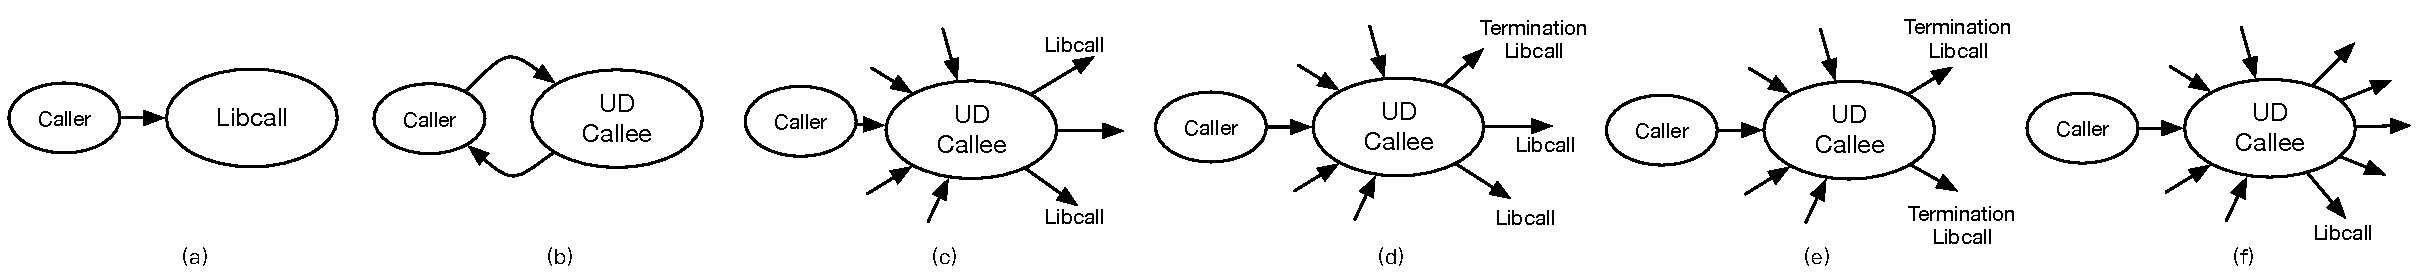
\includegraphics[width=\textwidth]{srj-figures/srj-caller-callee6.pdf}
  %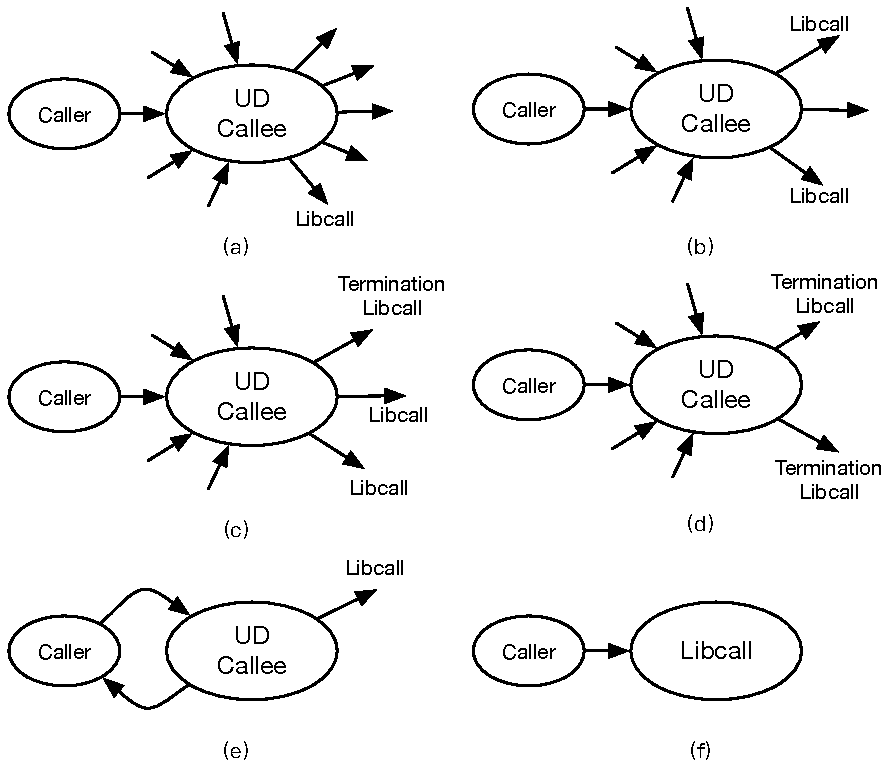
\includegraphics[width=0.45\textwidth]{srj-figures/srj-caller-callee4.pdf}
  \caption{Commonly observed function invocation patterns, where `UD' denotes user-defined callee function. Here, all the incoming and outgoing edges (or calls) represent user-defined functions, unless specified as \textit{Libcall} or \textit{Termination Libcall} next to them} \label{fig:caller-callee} \vspace{-1mm}
\end{figure*}
In order to inline relevant functions, we use the function invocation patterns to guide the inlining decision. Based on our study, six commonly-observed invocation patterns are identified and summarised in Fig.~\ref{fig:caller-callee}.
Incoming (outgoing) edges in Fig.~\ref{fig:caller-callee} represent the incoming (outgoing) calls to (from) the function.
%Four out of six patterns refer to the functions to be inlined, while the other two are not.
Here, we elaborate the six patterns as follows.

\noindent\textbf{Case 1:} Fig.~\ref{fig:caller-callee}(a) depicts the direct invocation of standard C library function(s) by the caller function under investigation. To recover the semantics, it is essential to understand the semantics of called library function(s). Hence, the library function is inlined into the caller function.  Currently, we only consider the most common standard C library functions --- in total 60 functions,
%(e.g., \texttt{memcpy} and \texttt{strlen})
from both Linux (\texttt{libc}) and Windows (\texttt{msvcrt}), for inlining. This list can be further extended when necessary.

\noindent\textbf{Case 2:} Fig.~\ref{fig:caller-callee}(b) depicts the case of a recursive relationship between the caller and the UD (user-defined) callee function $f$. Hence, we inline $f$ into its caller. Note that the recursive functions are, unlike in compilers, inlined only once. For example, \texttt{gcc} has a default inlining depth of 8 for recursive functions.

\noindent\textbf{Case 3:} Fig.~\ref{fig:caller-callee}(c) depicts the common pattern of a \textit{utility function} --- e.g., the UD callee function $f$ is called by many other UD functions, while $f$ calls several \textit{library functions} and a very few (or zero) UD functions. This suggests that $f$ is behaving as a utility function, as $f$ has some semantics that is commonly needed by other functions, and hence $f$ is likely to be inlined.
% into its caller.
% depending on the number of other UD functions `referred to' by this callee (lower the reference to other UD functions, better chance of inlining).}

\noindent\textbf{Case 4:} The UD callee function $f$ in Fig.~\ref{fig:caller-callee}(d) is a variant of~\ref{fig:caller-callee}(c), where it has several references to library functions and \textit{zero} reference to other UD functions. Such zero reference to UD functions makes $f$
%carries some unique semantics --- called \textit{unique function},
an ideal candidate for inlining. Note that $f$ is inlined as the majority ($50\%$ or more) of its invoked library functions are not of termination type. Hence, we can safely assume that $f$ is doing much more than just facilitating program termination. Here, termination type refers to the library functions that lead to exceptions or program termination (e.g., \texttt{exit} and \texttt{abort}).

\noindent\textbf{Case 5:} In Fig.~\ref{fig:caller-callee}(e), The UD callee function $f$ is a variant of~\ref{fig:caller-callee}(d), which has only references to library functions.
% and \textit{zero} reference to other UD functions.
However,  all the invoked library functions in $f$ are of termination type. Hence, we consider as a function that facilitates only program termination (or exception handling) and its semantics are of little interest to the caller, which should not be inlined.

\noindent\textbf{Case 6:} Fig~\ref{fig:caller-callee}(f) depicts the scenario of a \textit{dispatcher function}  where the UD function $f$  is called by (i.e., incoming calls) many other UD functions and $f$ itself calls many other UD and library functions. In this case, $f$ appears to be a dispatcher function without much unique semantics, and hence, in most cases, not inlined.
%within the caller.

%\xyx{\textbf{Mahin, we need the example and some statistics for the above 4 cases. With the good example and solid empirical statistics, reviewers are prone to buy the following algorithm.}}


%\begin{MyAlgo}[t]{-5.5cm} %increase or decrease margin, span across columns
\begin{MyAlgo}[t]{-4.9cm} %increase or decrease margin, span across columns
\scriptsize
 \DontPrintSemicolon
 \KwData{caller $\mathcal{F}$, set of callee functions $\mathcal{C}$, set of termination lib. func. $\mathcal{L}_t$, set of inlining lib. func. $\mathcal{L}_s$}
 \KwResult{inlined function $\mathcal{F}^I$}
 \SetKwFunction{algo}{$\mathtt{SelectiveInline}$}\SetKwFunction{proc}{Extract}
 \SetKwProg{myalg}{Algorithm}{}{}
 \myalg{\algo{$\mathcal{F},\mathcal{C}, \mathcal{L}_s, \mathcal{L}_t$}}{
   %$\Re \longleftarrow \emptyset$ \;
   %$\Re_M \longleftarrow \emptyset$ \;
   %$\mathtt{dict[\cdot]=\lbrace\rbrace}$ \tcp*{n-gram dictionary}
   \ForEach{{\upshape function} f {\upshape in } $\mathcal{C}$}{
   \tcp{inline selected library functions}
   \uIf{$ f \in \mathcal{L}_s$}{
  		$ \mathcal{F}^I \longleftarrow \mathcal{F}.\mathtt{inline}(f)$\;
  		\Return $\mathcal{F}^I$ \;
	}
	\uElseIf{$f \notin \mathcal{L}_s$ { \upshape \&\& } $\mathtt{isLibCall}(f)$}{
		\Return null\;
	}
	 \tcp{for all other user-defined callee functions}
  % \tcp{below $O_u^f, O_l^f$ refers to outgoing user-defined, library func. calls and $I_u^f$ refers to incoming user-defined func. calls}		
   $I_u^f \longleftarrow \mathtt{getIncomingCalls}(f)$ \;
   $O_u^f, O_l^f \longleftarrow \mathtt{getOutgoingCalls}(f)$ \;
   $O_u^f \longleftarrow O_u^f \backslash \mathcal{F}$ \tcp*{remove recursion}	
   %\eIf{$\vert O_u^f \vert == 0$ \&\& $O_l^f \in \mathcal{L}_t $}{
   \eIf{$\vert O_u^f \vert == 0$ { \upshape \&\& } $(\vert O_l^f \cap \mathcal{L}_s\vert - \vert O_l^f \cap \mathcal{L}_t \vert )\leqslant 0 $}{
  	%$\mathtt{\textbf{return}}$ \; \label{algo2:abAPI}
  	\Return null\;
	}{
	%\tcp{measure of utility function}
	%\tcp{all other calls are considered function calls}	
  	%\xyx{$\lambda_a = \vert I_u^f \vert$ ,  	$\lambda_e = \vert O_u^f \vert$, 	$\alpha = \lambda_e/({\lambda_e + \lambda_a})$}\;
  	$\alpha = \lambda_e/({\lambda_e + \lambda_a})$ \textit{\: where} $\lambda_a = \vert I_u^f \vert$, $ \lambda_e = \vert O_u^f \vert$\;
  	%\tcp*{incoming user-defined func. calls}
   %\tcp*{outgoing user-defined func. calls}

  	%\tcp{lower the $\alpha$, $f$ is likely to be inlined into $\mathcal{F}$}
  	\tcp{lower the $\alpha$, function $f$ is likely to be inlined}
  	\eIf{$ \alpha >$ {\upshape threshold } $t$ { \upshape \&\& } $\mathtt{notRecursive}(\mathcal{F},f)$}{
  		%$\mathtt{\textbf{return}}$ \; \label{algo2:abAPI}
  		\Return null\;
		}{
		%\tcp{all other calls are considered function calls}	
  		$ \mathcal{F}^I \longleftarrow \mathcal{F}.\mathtt{inline}(f)$\;
  		\eIf{$ \vert O_u^f \vert > 0$}{
  		$\mathtt{SelectiveInline}(f,O_u^f,\mathcal{L}_s, \mathcal{L}_t)$\; \label{algo2:abAPI}
		}{
		\Return $\mathcal{F}^I$ \;
		}
 		}
  	}
}
\Return $\mathcal{F}^I$ \;
}
 \caption{Selective inlining algorithm}\label{algo:select-inline}
\end{MyAlgo}

\subsection{Inline Decision Algorithm}

From the discussions above, in Fig.~\ref{fig:caller-callee} (a), (b), (d) and (e) there is a clear criterion in deciding whether a callee
%\xyx{(no matter user-defined or library function)}
should be inlined or not.
%For \ref{fig:caller-callee}(c) (Case 4), we inline the callee, if the total number of termination type library functions are smaller than interesting library functions .
However, for Fig.~\ref{fig:caller-callee} (c) and (f), the most commonly observed invocation patterns, a systematic decision-making procedure is still needed.
To identify the cases of commonly-used functions (i.e., utility functions) to be inlined, we borrow the \textit{coupling} concept from the software quality and architecture recovery community. In software metrics, the coupling between two software packages is measured by the dependency between them, e.g., the software package instability metrics~\cite{martin2003agile}. In this work, similarly, we measure the function coupling by the \textit{function coupling score}. % to decide whether a callee should be inlined or not, which is formally defined as follows.

\begin{mydef} \label{def:comp_semantic}
\emph{\textbf{Function Coupling Score}}
refers to the complexity of the invocations involved in a function and is calculated as $\alpha = \lambda_e/({\lambda_e + \lambda_a})$,
%\begin{equation}
%\begin{aligned}
% \alpha = \frac{\lambda_e}{\lambda_e + \lambda_a}
%\end{aligned}
%\end{equation}
where $\lambda_a$ represents the number of UD functions that refers to the callee, and  $\lambda_e$ represents the number of UD functions that is referred to by the callee.
\end{mydef}
The lower the value of $\alpha$, more likely the callee should be inlined. The rationale is that the low function coupling score implies the high independency of the functionality ---  the high possibility of being utility function.
%For example, when the callee doesn't refer to any other UD functions (i.e., $\lambda_e = 0$), it is assumed to be behaving as autility function (where, $\alpha = 0$) and hence, inlined.
When calculating $\lambda_e$, we only consider the UD functions invoked by the callee, not the library functions. As mentioned in case 3 (Fig.~\ref{fig:caller-callee}(c)) and 6 (Fig.~\ref{fig:caller-callee}(f)), it is the invocations of UD functions that indicate the behavior of the callee as a dispatcher or a utility function, not the invocations of library functions.

%\xyx{\textbf{Mahin, need to give $\alpha$  for (a) to (b).}} \mahin{yes, I'll include after exp.}

The proposed selective inlining process is presented in Algorithm~\ref{algo:select-inline}. As first, if the callee is one of the selected library functions (e.g., \texttt{memcpy} and \texttt{strlen} as in case 1), it is directly inlined into the caller (lines 3-5) and rest of the library functions are ignored. Next, the UD functions that refer to the callee is denoted as $I_u^f$; while the library and UD functions  referred to by the callee are identified and denoted as $O_l^f$ and $O_u^f$, respectively at line 8-9. Callee that invokes only library functions that are of termination type is not inlined (lines 11-12). Finally, for the rest of the callee functions, the function coupling score is calculated and if it is  below some threshold value $t$, the callee is inlined (lines 13-24). This recursive procedure is continued until all the related functions are analysed.
%\textbf{Mahin, how to distinguish b, c and d is not clear.}

In our preliminary study on BusyBox compiled for x86 32bit, we identify that 14 UD utility functions (case 3) have more than 50 incoming calls with 1 outgoing call, while 12 UD dispatcher functions (case 6) have more than 50 outgoing calls with just 1 incoming call.  Similarly, in BusyBox compiled for ARM, we identify such 15 UD utility functions but only 4 UD dispatcher functions. This clearly differentiates the function invocation patterns case 3 (Fig.~\ref{fig:caller-callee}(c)) and 6 (Fig.~\ref{fig:caller-callee}(f)).
In this work, we adopt a lightweight static analysis to make the inlining decision for the performance reason (as shown in Section~\ref{sec:experiemntation}).
A more expensive program analysis can be used to improve the accuracy, but we strike for the balance between performance and accuracy in this work.



 %The rationale is that the emulation step is after the selective inlining step, and the important function calls have been retained. For those function calls after selective inlining,  these functions as well as other functions they called will be all inlined.

%srj
%aum gaanathipathaye namaha
 %aum gaanathipathaye namaha
%srj


\section{Scalable Function Matching}\label{sec:func_match}
%This section, we present the four modules in \tool in details.
%As the first step, \tool disassembles the binary and splits it into basic functional units or functions. Then, it constructs the control-flow graph (CFG) for each function, where each CFG is consists of basic-blocks. Later, the constructed CFGs are used to generate the partial traces.

%\subsection{Partial Trace Extraction} \label{subsec:partial_trace}

In \tool and \toolNew, similarity matching is done at the granularity of function and sub-function levels (i.e., we can match a part of a target function to the signature function).




\subsection{Primary Matching} \label{subsec:matching:primary}
In primary matching, high-level semantic features and structural features are combined to measure the semantic similarity of the two code segments as the granularity of function. Let $\mathcal{SIM_{H}}(sig, tar)$  denote the similarity score of using high-level semantic features and $\mathcal{SIM_{S}}(sig, tar)$ denote the similarity score of using structural features.
The former score is measured by Jaccard containment similarity~\cite{agrawal2010indexing}, considering each function has a bag of high-level semantic features:
\begin{equation}
\begin{aligned}
\mathcal{SIM_{H}}(sig, tar) = \frac{\mathcal{H}_{sig} \bigcap \mathcal{H}_{tar}}{\mathcal{H}_{sig}}
\end{aligned}
\end{equation}

\xyx{Specifically, for each of six types of high-level semantic features, the Jaccard distance is calculated, and the overall $\mathcal{SIM_{H}}(sig, tar)$  is the mean value of Jaccard distances of different types of high-level semantic features. Note that if both signature function and target function have no function calls, then features in terms of function call tags, function call sequence, function parameters are not available, and they are not counted in overall similarity.}

The latter score is measured by calculating FDD (Definition 3 in \S\ref{sec:category:structralFea}), and the FDD value is already normalized into  the range between 0 to 1. $\mathcal{SIM_{S}}(sig, tar)$ is to convert the distance to the similarity:
\begin{equation}
\begin{aligned}
 \mathcal{SIM_{S}}(sig, tar) = Convert(FDD(sig, tar)) \\
 = 1 - FDD(sig, tar)%\frac{FDD(sig, tar)}{w'_{sig} + w'_{tar}}
\end{aligned}
\end{equation}
%\begin{equation}
%\begin{aligned}
% Norm(FDD(sig, tar))
%\end{aligned}
%\end{equation}
%where $w'_{sig}$ and $w'_{tar}$ denote the number of weighted assembly instructions in function $sig$ and function $tar$, respectively.
The idea of convertion is that if these two functions' distance is closer to 0, their similarity is closer to 1. Vice versa, if their distance is as big as it could possibly be, their similarity is prone to be 0.

Once we have similarity scores in high-level semantics and structures, the primary matching result $\mathcal{SIM^\prime}(sig, tar)$ is calculated as the weighted sum of $\mathcal{SIM_{H}}(sig, tar)$ and $\mathcal{SIM_{S}}(sig, tar)$, which is defined as follow:
\begin{equation}
\begin{aligned}
 \mathcal{SIM^\prime}(sig, tar) =  (1 - \mathcal{W}/2) *  \mathcal{SIM_{H}}(sig, tar)  \\
  + ( \mathcal{W}/2) * \mathcal{SIM_{S}}(sig, tar)
\end{aligned}
\end{equation}
where $\mathcal{W}$ = $min(\frac{w'_{sig}}{ w'_{tar}}, \frac{w'_{tar}}{ w'_{sig}})$ and $\mathcal{W}$ means the ratio of these two functions' instruction number.

Hence, the idea of primary matching is straightforward --- structural features are effective when the sizes of two functions are similar. If two functions have the similar size of instructions, structural features have the same weight as high-level semantic features. If not, high-level semantic features have more weight than structural features. According to this idea, a high value of $\mathcal{SIM^\prime}(sig, tar)$ (e.g., $\geq 0.8$) indicates that $sig$ and $tar$ are similar in both structures and high-level semantics.

\subsection{Low-level Semantic Features Matching} \label{subsec:matching:lowFea}
%\footnote{Signature function refers to the search query function in hand, whereas target functions refer to functions in the target binary pool against which the signature function is matched.}
When the primary matching does not find any ranked results that are of high $\mathcal{SIM^\prime}(sig, tar)$ values, low-level semantic features are used.
Note that low-level semantics refer to not only the implementation details, but also the partial semantics of the function.
To this end, we propose the function model consisting of partial traces of various lengths, %, a variant of tracelet~\cite{DBLP:conf/pldi/DavidY14},
which is more flexible in terms of comparison granularity, compared with the BB-centric
%and tracelet~\cite{DBLP:conf/pldi/DavidY14} based
function modelling~\cite{DBLP:conf/sp/PewnyGGRH15,luo2014semantics}. Then, from these partial traces we extract symbolic expressions. Based on I/O values for register, flags and memory addresses, we match the partial traces inside two functions. %To reduce the noise, we remove the partial traces that are infeasible to reach (via solving the symbolic expressions) or are specific to compilers.
Last, we apply Jaccard containment similarity~\cite{agrawal2010indexing} to measure the similarity score of two function models.
%That is, for each function, we generate partial traces of various lengths (called, \textit{k-length partial traces}), where by varying the length, the semantics of the function is captured at various granularity levels.
%granularity of single building block is adjusted\footnote{Length of one yields a basic-block centric models, where the basic-block is considered as a single building block.}.
\subsubsection{K-length Partial Trace Extraction} \label{subsec:partial_trace_ext}
Our partial trace extraction is based on the technique proposed by David \emph{et. al.}~\cite{DBLP:conf/pldi/DavidY14}.
We omit the algorithm and explain the results using one example.
Fig.~\ref{fig:example-cfg} depicts a sample CFG of a function and the extracted 2- and 3-length partial traces (i.e., for $k=2,3$). We can observe that the original control-flow instructions (\texttt{jnb}, and \texttt{jb}) are omitted as the flow of execution is already determined. Note that the feasibility of the flow of executions is not considered at this step. %In \S\ref{subsubsec:sou_prun}, we show how the partial traces which are \textit{infeasible} to reach are identified via constraint solving and removed. %from our analysis. Here, infeasible partial traces refer to program execution flows that are not possible to reach during any concrete execution.

\begin{figure}[]
\begin{center}\vspace{-3mm}
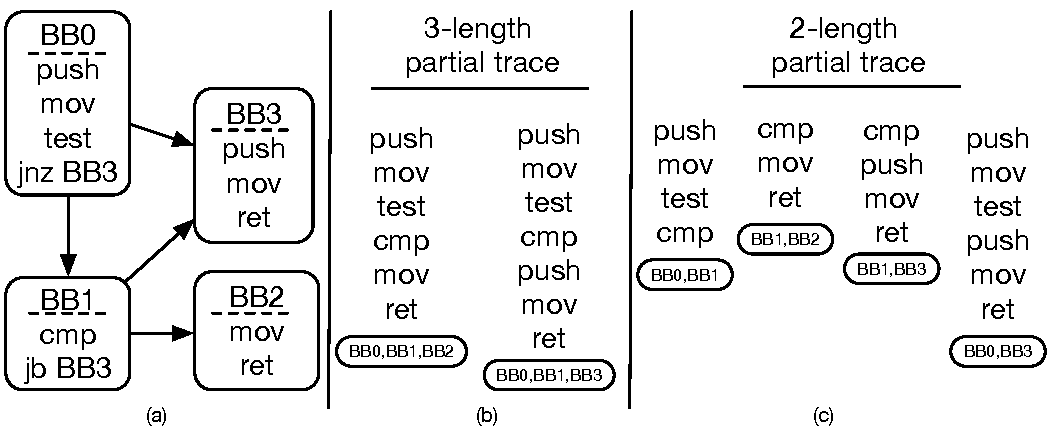
\includegraphics[width=7.5cm]{srj-figures/srj-partial_trace_ex.pdf} %\vspace{-1mm}
\caption{A sample CFG (a) and the extracted 3-length (b) and 2-length (c) partial traces}
\label{fig:example-cfg} \vspace{-2mm}
\end{center}
\end{figure}
%
%\subsection{Trace Pruning}\label{subsec:trace_prun}
%In \tool, we adopt two trace pruning methods to reduce the noise in the results and also to speed up the matching process.
%%steps to reduce the noise in I/O samples based function \textit{similarity} matching, which is less precise than the unscalable function \textit{equivalence} matching.}
%\subsubsection{Infeasible Partial Trace Pruning} \label{subsubsec:sou_prun}
%\tool is a static analysis based tool, and therefore it is difficult (or even impossible) to identify all the infeasible partial traces in practice. In \tool, we prune the obviously infeasible partial traces via the constraint solver. Given the symbolic expressions extracted from a partial trace, we rely on the constraint solver to determine whether all the constraints present in the symbolic expressions can be satisfied. %If not, that relevant partial trace is considered infeasible.
%As we use the constraint solver to generate I/O samples in \S\ref{subsec:sem_fea_ext}, we need no additional effort to identify the infeasible partial traces --- if the constraint solver is unable to find appropriate concrete values for the pre- and post-state variables, the relevant partial trace is considered infeasible.
%%That is, given a partial trace, we extract the set of I/O formulas, as explained in Section~\ref{subsec:stat_sem}, and try to generate a model that satisfied all the constraints present in the I/O formulas (i.e., able to generate appropriate concrete values for input/out vocabularies), if such model is not available then that partial trace is considered infeasible.
%%and pass them to the solver, which will try to solve the constraints and generate a model that satisfies them all. If the solver fails to generate a model, we label that partial trace as infeasible and prune it from the analysis.
%
%We also observe that some  partial traces, for which the solver is able to generate models (or I/O samples), might be infeasible during actual execution, as the feasibility of their paths depends on various factors, such as global variables, values in the heap and other dynamic data, that are beyond the scope of our analysis. Further, in general, infeasible path elimination (or detection) by itself is a hard problem~\cite{bodik1997refining}. However, compared with the static analysis solutions proposed in the literature~\cite{DBLP:conf/pldi/DavidY14,pewny2014leveraging,DBLP:conf/sp/PewnyGGRH15}, this work makes an attempt to reduce the search candidates using a pruning technique.
%
%%Even with the infeasible partial traces pruned, it is still difficult to compare the signature function against those functions in the target binary pool. Thus, a systematic way of performing the similarity matching among partial traces is desired. Specifically, the question ``what length of partial traces in the search query needs to be matched with what length of partial traces in the target function?'' still persists.
%
%
%
%
%\subsubsection{Compiler Specific Code Pruning}
%%%Compiler idioms capture the compilation information, via code patterns  commonly  included for a specific compilation option during compilation process.
%%%\noindent \textbf{Compiler idiom}
%%%These idioms help to identify the additional code included by the compiler during compilation process.
%Based on the compilation option selected, the compiler could include additional code (i.e., code that is not originally written by the programmer) into the compiled binary. For example, there are more than 150 compiler options available for both \texttt{gcc} and \texttt{MS Visual Studio}, which a programmer can choose from when compiling her program. Some of these options result in adding extra code into the binary (e.g., \texttt{stack-smashing protection} or SSP shown in Fig.~\ref{fig:gcc_ssp}). The code segments in the function prologue and epilogue in Fig.~\ref{fig:gcc_ssp} ensure the stack integrity is not violated. These code segments are automatically included by the \texttt{gcc} compiler when the option for stack smash protection is enabled.
%%(using either \texttt{-fstack-protector-all} or \texttt{-fstack-protector} flag).
%%(using either -$\mathtt{fstack}$-$\mathtt{protector}$-$\mathtt{all}$ or -$\mathtt{fstack}$-$\mathtt{protector}$ flag).
%
%In similarity matching between the signature and target functions, the additional compiler specific code can introduce noise by changing the code structures and diluting the similar parts, especially when the functions are small.
% %the additional code included by the compiler might influence the similarity score between the signature and target functions, especially when the functions are relatively small.
%% Therefore, in order to avoid imprecise similarity matching, the compiler specific code need to be removed from the partial traces.
%Thus, it is necessary to identify and remove the compiler specific code from the partial traces.
%However, directly removing some code from a partial trace might lead to incorrect semantic features, as these features are very sensitive to the underlying code semantics.
%
%To this end, we propose a conservative approach to address this problem by generalizing the compiler specific code into some patterns and systematically pruning the partial traces that contain these patterns.
%%, as in~\cite{rosenblum2008learning},
%%The partial traces that contain these patterns are systematically pruned.
%That is, instead of removing the compiler specific code from a partial trace, which is error prone, we just remove the partial trace itself if the compiler specific code pattern accounts for the majority (50\% or more) of the code. As an initial step, we only consider three types of compiler specific code patterns (i.e., SSP, function prologue and epilogue) that are very commonly observed in the binaries. This list can be further extended when necessary.
%of the code present in a partial trace, the partial trace is completely removed from the analysis.
%This approach does not eliminate the whole the problem but tries to minimize the effect of compiler specific code influencing the final similarity score.



%Interestingly, some compiler idioms help to understand more about the program. For example, the presence of SSP in selected functions (i.e., -$\mathtt{fstack}$-$\mathtt{protector}$ compiler feature) in a program indicates that these  functions have buffers larger than 8 bytes. Compiler idioms are architecture- and OS-specific, however, their high-level meanings are unified across architectures and OSs.


\subsubsection{Function Model Generation} \label{subsec:fun_mod_mat}

\begin{figure}[t]
  \centering
  %width = 7cm,
  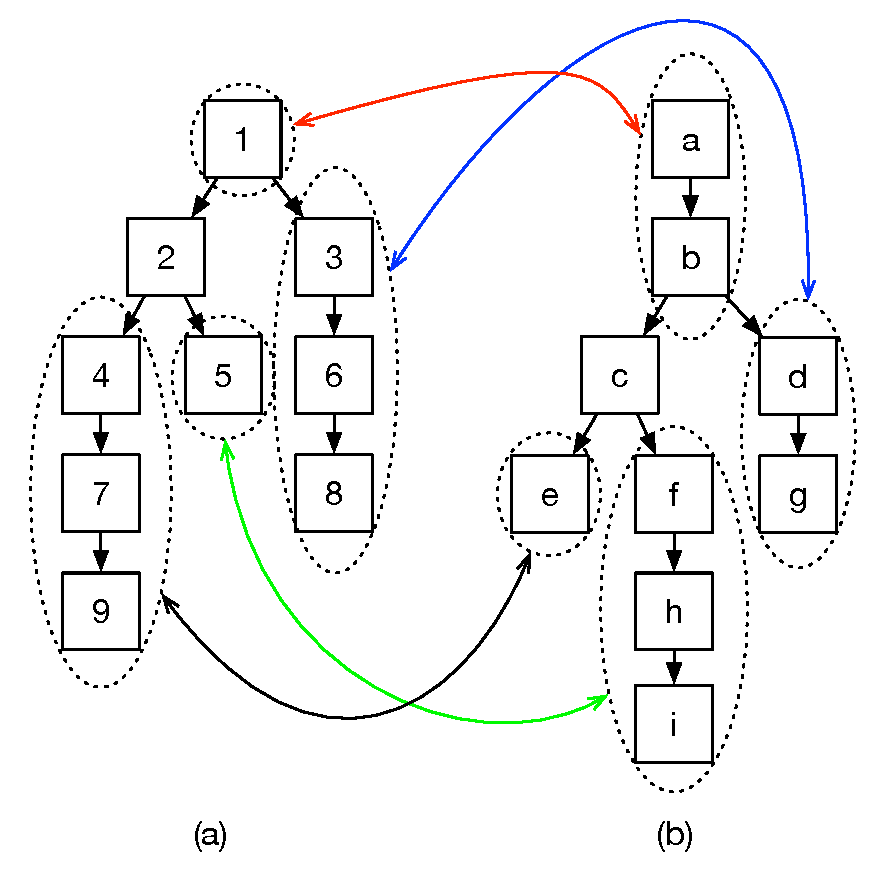
\includegraphics[width = 5cm,height=4cm]{srj-figures/srj-func_mod.pdf} %the_graph
  \caption{A sample signature (a) and target (b) functions, where the lines indicate the matched partial traces and the nodes refer to the basic-blocks.} \label{fig:func_mod}
%\vspace{-1mm}
\end{figure}


In \tool, we leverage on length variant partial traces to model the functions. %The key advantage of using partial trace over other techniques~\cite{DBLP:conf/pldi/DavidY14, DBLP:conf/sp/PewnyGGRH15,luo2014semantics,sebastian2016discovre} lies in its resilience to the structural changes. %To this end,
We generate partial traces with three different lengths (i.e., $k=1,2$ and $3$) from each function, all of which collectively constitute the function model. For example, function models generated from the signature ($\mathcal{M}_{sig}$) and target ($\mathcal{M}_{tar}$) functions in Fig.~\ref{fig:func_mod} are listed as follows:

\begin{itemize}
\small
\itemsep0em
  \item[] $\mathtt{\mathcal{M}_{sig}:  \lbrace \langle 1 \rangle,  \langle 2 \rangle,\ldots, \langle 1,2 \rangle, \langle 2,5 \rangle, \ldots, \langle 1,2,4 \rangle, \langle 2,4,7 \rangle,\ldots\rbrace}$
   \item[] $\mathtt{\mathcal{M}_{tar}: \lbrace \langle c \rangle,  \langle b \rangle, \ldots, \langle a,b \rangle, \langle b,c \rangle, \ldots, \langle a,b,c \rangle, \langle b,c,f \rangle, \ldots \rbrace}$
\end{itemize}

In \tool and \toolNew, we support the function model similarity matching in terms of \textit{n-to-m}, \textit{1-to-n}, \textit{n-to-1} and \textit{1-to-1} partial trace matching across the signature and target functions, mitigating the impact of program structural difference.
\begin{description}
\itemsep0em
  \item[\textit{n-to-m}] Partial traces of length $n (\in\mathbb Z_{> 1})$ generated from the signature function are matched against the partial traces of length $m (\in\mathbb Z_{> 1})$ generated from target function. In Fig.~\ref{fig:func_mod}, matching partial traces $\langle 3,6,8\rangle$ and $\langle d,g\rangle$ is \textit{3-to-2} matching.
  \item[\textit{1-to-n}] A basic-block (i.e., a partial trace of length 1) in the signature function is matched against the partial traces of   length $n (\in\mathbb Z_{> 1})$ generated from target function. In Fig.~\ref{fig:func_mod}, partial traces $\langle 1\rangle$ and $\langle 5\rangle$ are matched with $\langle a,b\rangle$ and $\langle f,h,i\rangle$, respectively.
  \item[\textit{n-to-1}] Partial traces of length $n (\in\mathbb Z_{> 1})$ generated from the signature function are matched against a basic-block in the target function. In Fig.~\ref{fig:func_mod}, partial trace $\langle 4,7,9 \rangle$ is matched with $\langle e \rangle$.
  \item[\textit{1-to-1}] A basic-block in the signature function is matched against a basic-block in the target function. It is also known as pairwise comparison at the level of single basic-block. In Fig.~\ref{fig:func_mod}, partial trace $\langle 2\rangle$ is matched with $\langle c\rangle$.
\end{description}

\textit{1-to-n} matching addresses the issue of basic-block splitting --- a single basic block in the signature function is split into several smaller basic blocks in the target function. Similarly, \textit{n-to-1} matching addresses the basic-block merging problem.
%On the other hand, \textit{n-to-m} mapping is generally preferred when the signature (target) function is part of a huge target (signature) function and appropriately selected values for $n$ and $m$ will maximize the function similarity. Finally, if none of the aforementioned matching techniques work, we resort to \textit{1-to-1} matching to compare the basic-block similarity in a pairwise way, which is similar to those basic-block centric comparison approaches~\cite{DBLP:conf/sp/PewnyGGRH15,luo2014semantics}.
In tracelet modeling \cite{DBLP:conf/pldi/DavidY14}, authors recommended that both the signature and target should be of the same size (i.e., $k=3$), and hence only \textit{n-to-n} matching is performed.
In~\cite{DBLP:conf/sp/PewnyGGRH15} and~\cite{luo2014semantics}, pairwise comparison of single basic-block (i.e., \textit{1-to-1} matching) is performed as an initial step to shortlist target functions. In contrast, in \tool and \toolNew, all the  4 types of function matching are needed to cover all possible BB-structure variances that arise due to architecture, OS and compiler differences.


For the similarity score of using low-level semantic features $\mathcal{SIM_{L}}(sig, tar)$, considering the function model as a bag of partial traces, Jaccard containment similarity~\cite{agrawal2010indexing} is also used to measure the similarity of two different function models:
\begin{equation}
\begin{aligned}
 \mathcal{SIM_{L}}(sig, tar)  = \frac{\mathcal{M}_{sig} \bigcap \mathcal{M}_{tar}}{\mathcal{M}_{sig}}
\end{aligned}
\end{equation}
where $\mathcal{M}_{sig}$ and $\mathcal{M}_{tar}$ refer to function models of low-level semantics that are generated from signature and target functions, respectively.

%
%Finally, considering the function model as a bag of partiral traces, Jaccard containment similarity~\cite{agrawal2010indexing} is used to measure the similarity score between  two different function models, and is defined below:
%\begin{equation}
%\begin{aligned}
% sim(\mathcal{M}_{sig}, \mathcal{M}_{tar}) = \frac{\mathcal{M}_{sig} \bigcap \mathcal{M}_{tar}}{\mathcal{M}_{sig}}
%\end{aligned}
%\end{equation}
%where $\mathcal{M}_{sig}$ and $\mathcal{M}_{tar}$ refer to function models generated from signature and target functions, respectively.

%In \tool, the function model matching is not fixed, where, for a given signature function, the searching algorithm will try all possible function models and pick the best one that maximizes the signature-target function similarity. In contrast, the techniques proposed in the literature do not have the flexibility to try out all possible matchings. For example, in tracelet-based modeling \cite{DBLP:conf/pldi/DavidY14}, the authors recommended that the tracelet size should be larger (e.g., $k>2$), for both signature and target functions, hence, only \textit{n-to-m} matching is performed, in fact, it is \textit{n-to-n} matching as they consider the same tracelet size for both signature and target functions. Further, in~\cite{DBLP:conf/sp/PewnyGGRH15} and~\cite{luo2014semantics}, pairwise comparison of basic-blocks (i.e., \textit{1-to-1} matching) is performed as an initial step to identify potential target functions, which inherently assumes that the program structure is maintained across signature and target functions and at least one basic-block in the target function resembles a basic-block in the signature function.

%\subsection{Locality Sensitive Hashing} \label{subsec:lsh} %\note{replace this with simple feature hasing technique, if no time, leave as it is.. not very important}
%In \tool, we leverage on Locality-sensitive Hashing (LSH) technique to perform the function matching more efficiently and in a scalable manner. Locality-sensitive hashing is an algorithm for searching similar items in large and high dimensional dataset \cite{leskovec2014mining} based on the assumption that, if two items are similar, the hashed value of the two items will remain similar. In \tool, we use MinHashing~\cite{broder1997resemblance} technique to hash the extracted features and generate hash signature for each function model. To this end, we use 1000 (i.e., $n=1000$) hash functions to generate the signature, which leads to an error of 3.16\%. The similarity between two function model is given by this equation:
%\begin{equation}
%\begin{aligned}
% sim(mh_a, mh_b) = \frac{\vert mh_a[i]=mh_b[i ]\vert}{n}
%\end{aligned}
%\end{equation}
%where the jaccard similarity between two function models is approximated by MinHash similarity between the two models.

%\subsubsection{Function Model Generation} \label{subsec:fun_mod_mat}

%\subsection{Primary Matching and Final Matching} \label{subsec:sem_fea_ext}
%\subsubsection{Primary Matching}
\subsection{Final Matching} \label{subsec:matching:final}

To remove false positives of using low-level semantics alone, $\mathcal{SIM^\prime}(sig, tar)$ is also considered in the final matching.

Let $\mathcal{SIM^*}(sig, tar)$ denote the overall similarity score calculated in the final matching. $\mathcal{SIM^*}(sig, tar)$ is calculated as the weighted sum of $\mathcal{SIM^\prime}(sig, tar)$ and  $\mathcal{SIM_{L}}(sig, tar)$. Here, we adopt two strategies for different matching scenarios.

If the matching is based on the same code base, we consider both $\mathcal{SIM_{L}}(sig, tar)$ and $\mathcal{SIM^\prime}(sig, tar)$ are equally important.
\begin{equation}
\begin{aligned}
 \mathcal{SIM^*}(sig, tar) =  (1/2) * \mathcal{SIM^\prime}(sig, tar)  \\
  + (1/2) * \mathcal{SIM_{L}}(sig, tar)
\end{aligned}
\end{equation}


Otherwise, if the matching is based on different code bases (i.e., experiments on cross-OS matching), we ignore the structural features and give equal weight for low-level semantics and high-level semantics.
\begin{equation}
\begin{aligned}
 \mathcal{SIM^*}(sig, tar) =  (1/2) * \mathcal{SIM_H}(sig, tar)  \\
  + (1/2) * \mathcal{SIM_{L}}(sig, tar)
\end{aligned}
\end{equation}

\xyx{Still take the code segments in Fig.~\ref{fig:falseposi} as example. The two code segments are from different code bases, and hence the BB structure will not be similar. Low-level semantics and high-level semantics are used together to measure their semantic similarity. Previously,  in \tool, using low-level semantics alone suggests they have a similarly value of 0.7 --- 70\% of tracelets in the signature function match the target function on I/O value pairs. Now, in \toolNew, since they have a low high-level similarity of 0.7 and no similarity in high-level features and structural features, their overall similarity is lower to 0.35. Hence, the false positive has a lower similarity score, and will be removed from the best-match or top-5-match list.}


%srj
%aum gaanathipathaye namaha


%
%\begin{figure}[t]
%\begin{center}%\vspace{-1mm}
%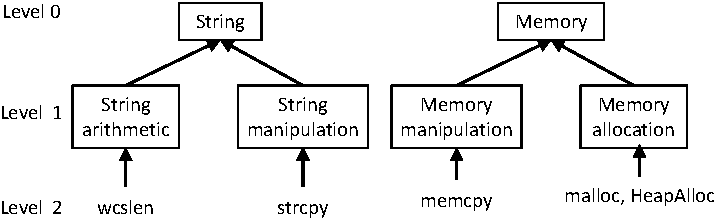
\includegraphics[width=0.4\textwidth]{srj-figures/srj-abs-1.pdf}
%%\vspace{-1mm}
%\caption{Library function abstraction levels}
%\label{fig:abs} \vspace{-2mm}
%\end{center}
%\end{figure}
%
%

%\subsection{Emulation}\label{sec:scalable:emulation}
%\subsection{Function Filtering}\label{sec:prefilter}

%%In practise, %to effectively search for a semantically similar function from a pool of several hundred thousand (or more) target functions compiled for various architectures and OS using different types of compilers with varying optimization levels,
%To deal with a huge number of target functions in real-world binaries, an effective filtering process can remove irrelevant target functions before the expensive matching step.
% \tool leverages on three types of filters, starting from the specific one to the most general one, to shortlist the candidate target functions. \\
%
%\noindent \textbf{Filter 1}: The first type of filters %\xyx{(\textit{aka.,} precise)}
% looks for identical library call invocations in the target functions according to the signature function. If the identical invocations are found, the corresponding targets functions are good candidates for further matching. The reason is that the library call invocations provide an important partial semantics of the function.
%However, this filter is OS dependent and fails to support library calls that have different names yet with similar functionality (e.g., \texttt{memcpy} and \texttt{memmove}).
%%Library calls can be inlined by the compiler or programmers might implement the same functionality in user-defined functions. Thus, relying on library call names will fail. %In addition, the given function may not invoke any library call at all, in such situations, library call based filtering is not helpful.
%
%\noindent \textbf{Filter 2}: To address the problem in library call name matching, we consider the library call operation types, which help to match the high-level functionality of the library calls. As shown in Fig.~\ref{fig:abs}, there are several ways of abstracting the functionality of a library call. Abstraction level 0 gives the base operation type (e.g., \textit{string} operation), while level 1 gives a more concrete but general abstraction supported cross all OSs.
%For example, \texttt{strcpy} and \texttt{strcat} can be mapped to \textit{string manipulation} operation. Therefore, we adopt abstraction level 1 to summarize the library function behavior. In addition, filter 2 is OS neutral, where functions that perform similar task but with different names across OS are mapped to the same operation type, e.g., \texttt{malloc} (Windows/Linux) and \texttt{HeapAlloc} (Windows) are mapped to \emph{memory allocation} operation type as shown in Fig.~\ref{fig:abs}.
%%\ly{I want to highlight this filter 2 is OS neatural and use one example to show it in fig 4. Also we should say we maintain the mapping ourself.}
%%in this study.
%%\todo{Include example for op. type mapping}
%
%However, library calls can be inlined by the compiler or programmers might implement the same functionality in user-defined functions. Thus, relying on library call names or the operation type will fail. To address this, we propose filter 3.%In addition, the given function may not invoke any library call at all, in such situations, library call based filtering is not helpful.
%
%
%\noindent \textbf{Filter 3}: %To address these serious issues of the first two filters, we \xyx{propose}
%The third filter is designed look for similarities in the instruction types involved in a binary function as a whole. Here, instruction type refers to a high-level operation carried out by an instruction~\cite{kruegel2005polymorphic}. In total, instructions are categorized into 14 and 8 instruction types for Intel and ARM architectures, respectively. For example, \texttt{mov} instruction is mapped to \textit{data movement} instruction type while \texttt{push} is mapped to \textit{stack operation}.
%In addition, instruction types also support cross-architecture function matching, where assembly instructions from ARM and Intel architectures are mapped to the same instruction type even though they are not identical at the instruction level (e.g., \texttt{call} (Intel) and \texttt{bl} (ARM) can be mapped to \textit{invoke function} instruction type).
%
%Nevertheless, this filter may suffer from the problem of semantics matching --- the instruction types used to implement the functions might look very similar even though they have totally different functionalities at a higher level.
%Since the filtering process is to shortlist all the target functions that are similar to the signature. %, and hence similarity at the instruction level is also very relevant even though they might be different at the high-level function behaviour.
%%This conservative approach is adapted not to miss any potential target functions.
%For the propose of not missing any potential target functions, some semantically irrelevant functions are tolerated in this step. \\
%
%
%\noindent \textbf{Filtering Algorithm} Filter 1 is specific and OS dependent. Filter 2 and 3 are general and cross-OS and cross-architecture.
%Our filtering process is shown in Algorithm~\ref{algo:pre-filt}.
%At lines 7,9 and 11, we use Jaccard distance~\cite{cha2007comprehensive} to measure the similarity between the signature and target functions in terms of each  filter, i.e., their similarity in identical library calls, in library call operation types, and in instruction types.
%Following the design of applying the filters one by one from the most specific one to the general one, we set the weights ($w_1 > w_2 > w_3 >0$ ) to the similarities achieved by Filter 1 to 3. At line 12, we sort the candidate functions according to the overall similarity on three filters (calculated at line 10). Finally, at line 13, we get the top $N$ of the sorting results and use them for function model matching.
%%\xyx{\textbf{give concrete value in implementation, discuss about the weight set in threat to validity!}}% where filter 1 is the most precise with  $w_1=1.0$, and filter 3 is the least precise with $w_3=0.5$ while filter 2 being in the middle with $w_2=0.8$.
%Note that our filtering process is performed after selective inlining step, hence we keep a mapping from the candidate function to its invoked libraries in order to apply the filters.
%%\todo{mention how NDSS 2016 gonna fail in pre-filtering}, \xyx{Mahin, maybe we can put all the comparison with NDSS paper in related work.}
%
%%sIn addition, we use inlined target functions, which helps to
%
%%It is important to note that, for each library call, we obtain the corresponding instruction types from the actual implementation of that library function in \texttt{libc} and \texttt{msvcrt}, for Linux and Windows binaries, respectively.
%
%
%%To make \tool capable of analyzing cross-OS binaries, we use a multi-level abstraction function $\mathtt{abstractSystemAPI}$ at line \ref{algo2:abAPI} to abstract system APIs based on their type. For example, the system API (or library call) \texttt{strlen} deals with string objects, and hence  the API can be naturally abstracted to `string' type. To this end, we use two levels of granularity (i.e., level 0 and 1) to abstract the system APIs, where each abstraction level play a different role in \tool~ --- abstraction level 0 abstracts the system API to their basic type, whereas level 1 provides more meaningful information about the API. For example, using our abstraction function, the system APIs \texttt{strlen}, \texttt{strcpy} and \texttt{strncpy} can be abstracted into two levels shown in Fig.~\ref{fig:abs}.
%
%
%%Based on the requirement of the analyst, there may be several ways to abstract a system API. As shown in Fig.~\ref{fig:abs}(b), abstraction level 1 can be more expressive in providing more meaningful information about the API or it can be limited as in Fig.~\ref{fig:abs}(a). One of the key applications of abstraction level 0 is that it is mostly used in pre-filtering process, where if a signature involves string manipulation operations then it is wise to quickly retrieve the target programs that also involve string manipulations. Similarly, abstraction level 1 is used to precisely match the signature with the target programs, where it can be used to specify additional constraints for the matching process. Level 1 abstraction is quite useful for vulnerability signature matching, e.g., the analyst can remove functions, from the filtered target programs, that use secure system API (e.g., \texttt{strncpy}, \texttt{\_\_strncpy\_chk,}etc.\footnote{With \texttt{FORTIFY\_SOURCE} compiler feature, whenever possible, \texttt{gcc} tries to uses buffer-length aware replacements for functions like \texttt{strcpy}, \texttt{memcpy}, \texttt{memset}, \texttt{gets}, etc., which are more secure.}), which are less likely to contain an exploitable vulnerability.
%%\xyx{Our evaluation also showed that ...}
%%
%%\subsection{Cross-architecture, OS and compiler pre-filtering algorithm}
%%To this end, in \tool, we have proposed a across-architecture, OS and compiler friendly pre-filtering algorithm that can filer the candidate target functions in a scalable fashion.
%
%%
%%\begin{MyAlgo}[t]{-4.8cm} %increase or decrease margin, span across columns
%%\scriptsize
%% \DontPrintSemicolon
%% \KwData{signature function $f$, set of target functions $\mathcal{T}$}
%% \KwResult{set of candidate target functions $\mathcal{T}_c$}
%% \SetKwFunction{algo}{$\mathtt{FunFilter}$}\SetKwFunction{proc}{Extract}
%% \SetKwProg{myalg}{Algorithm}{}{}
%% \myalg{\algo{}}{
%%    %$f_{in} \longleftarrow \mathtt{getInlinedFunc}(f)$\;
%% 	$\mathcal{S} \longleftarrow \lbrace \rbrace$ \;
%% 	%$t_{in} \longleftarrow \mathtt{getInlinedFunc}(t)$\;
%%   \ForEach{{\upshape function} t {\upshape in } $\mathcal{T}$}{
%%  	$s^t \longleftarrow \emptyset$\; 	
%%   $\mathcal{L}_f \longleftarrow \mathtt{getLibFuncList}(f)$ \;
%%   %$t_{in} \longleftarrow \mathtt{getInlinedFunc}(t)$\;
%%   %\uIf{$\vert \mathcal{L}_f \vert > 0)$}{
%%   \ForEach{{\upshape libcall} l {\upshape in } $\mathcal{L}_f$}{
%%   	$s^t \pluseq w_1 * \mathtt{getLibFuncNameSim}(l,t)$ \;
%%   	$l^O \longleftarrow \mathtt{getOpType}(l)$\; 	
%%   	$s^t \pluseq w_2 * \mathtt{getLibFuncOpTypeSim}(l^O,t)$ \;
%%   	%$l^I \longleftarrow \mathtt{getInstType}(l)$\; 		
%%   	%$s^t \pluseq w_3 * \mathtt{getLibFuncInstrTypeSim}(l^I,t)$ \;
%%   }
%%   $s^t \pluseq w_3 * \mathtt{getFuncInstrTypeSim}(f,t)$ \;
%%   $S[t] = s^t$ \;
%%}
%%$\mathcal{S}^s \longleftarrow \mathtt{sortCanditTargetFunc}(S)$ \;
%%$\mathcal{T}_c \longleftarrow \mathtt{topNTargetFunc}(\mathcal{S}^s,\mathcal{N})$ \;
%%\Return ${\mathcal{T}_c}$ \;
%%}
%% \caption{Function Filtering Algorithm}\label{algo:pre-filt}
%%\end{MyAlgo}
%
%
%\begin{MyAlgo}[t]{-4.8cm} %increase or decrease margin, span across columns
%\scriptsize
% \DontPrintSemicolon
% \KwData{signature function $f$, set of target functions $\mathcal{T}$}
% \KwResult{set of candidate target functions $\mathcal{T}_c$}
% \SetKwFunction{algo}{$\mathtt{FunFilter}$}\SetKwFunction{proc}{Extract}
% \SetKwProg{myalg}{Algorithm}{}{}
% \myalg{\algo{}}{
%    %$f_{in} \longleftarrow \mathtt{getInlinedFunc}(f)$\;
% 	$\mathcal{S} \longleftarrow \lbrace \rbrace$ \tcp*{store similarity score}
% 	%$t_{in} \longleftarrow \mathtt{getInlinedFunc}(t)$\;
% 	%$\mathcal{L}_f \longleftarrow \mathtt{getLibFuncNameList}(f); \mathcal{O}_f \longleftarrow \mathtt{getLibFuncOpType}(\mathcal{L}_f); \mathcal{I}_f \longleftarrow  \mathtt{getFuncInstrType}(f) $
% 	Get the set of library call names $\mathcal{L}_f$, library call operation types $\mathcal{O}_f$ and function instruction type $\mathcal{I}_f$ from the signature function $f$. \;
%   \ForEach{{\upshape function} t {\upshape in } $\mathcal{T}$}{
%
%   $s^t \longleftarrow \emptyset$\; 	
%   $\mathcal{L}_t \longleftarrow \mathtt{getLibFuncNameList}(t)$ \tcp*{filter 1}
%   $s^t \pluseq w_1 * \mathtt{getLibFuncNameJaccardSim}(\mathcal{L}_f,\mathcal{L}_t)$ \;
%   $\mathcal{O}_t\longleftarrow \mathtt{getLibFuncOpType}(\mathcal{L}_t)$ \tcp*{filter 2}
%   $s^t \pluseq w_2 * \mathtt{getLibFuncOpTypeJaccardSim}(\mathcal{O}_f,\mathcal{O}_t)$  \;
%   $\mathcal{I}_t \longleftarrow  \mathtt{getFuncInstrType}(t)$  \tcp*{filter 3}
%   $s^t \pluseq w_3 * \mathtt{getFuncInstrTypeJaccardSim}(\mathcal{I}_f,\mathcal{I}_t)$ \;	
%   $S[t] = s^t$ \;
%
%}
%$\mathcal{S}^s \longleftarrow \mathtt{sortCanditTargetFunc}(S)$ \tcp*{sort target functions}
%$\mathcal{T}_c \longleftarrow \mathtt{topNTargetFunc}(\mathcal{S}^s,\mathcal{N})$ \;
%\Return ${\mathcal{T}_c}$ \;
%}
% \caption{Function Filtering Algorithm}\label{algo:pre-filt}
%\end{MyAlgo}

%\subsection{Micro Execution}\label{sec:microExe}



%aum gaanathipathaye namaha
%srj
\section{Experimental Results}\label{sec:experiemntation}
%(Reverse Engineering Intermediate Language)

%, which enables us to do cross-architecture and cross-OS analysis


\noindent \textbf{Implementation.} In \tool and \toolNew, we use IDA Pro to disassemble and generate CFGs from the functions in binaries. Partial traces are generated using the \textsc{Tracy} plugin\footnote{https://github.com/tech-srl/tracy}, where they are of three different lengths (i.e., $k$-tracelet with $k=1,2$ and $3$). In \tool, to facilitate analysis and feature extraction, similar to~the preprocessing in~\cite{DBLP:conf/sp/PewnyGGRH15} and~\cite{luo2014semantics}, we lift the assembly instructions to an architecture and OS independent intermediate language, REIL~\cite{dullien2009reil}. \xyx{In \toolNew, no intermediate language is necessary as constraint solving based on REIL is not needed}. All the experiments were conducted on a machine with Intel Core i7-4702MQ@2.2GHz with 32GB DDR3-RAM.

\vspace{1mm}
\noindent \textbf{Configuration.} For cross-architecture matching, experiments are conducted on the different executables (i.e., x86-32, x86-64, ARM version) of \texttt{coreutils}. For cross-compiler matching, experiments are conducted on the executables that are compiled from \texttt{coreutils} with the different combinations of adopted compilers (\texttt{clang} and \texttt{gcc}) and optimization levels (O0-O3). For cross-OS matching,  we are matching between functions between \texttt{msvcrt} (for Windows) and \texttt{libc} (for Linux), which are compiled from different code bases \xyx{with \texttt{gcc} for x86-32}. For these experiments, we previously conduct them to evaluate \tool; we also conduct them to evaluate how \toolNew improves. To evaluate the real-world application of \tool, we use the code of open source project vulnerabilities as signature to search for the similar vulnerability in commercial products (e.g., Adobe PDF Reader). For \toolNew, we search for similar functions in binaries of forked projects, and compare the results with \textsc{CoP}~\cite{luo2014semantics}.

\subsection{Research Question}\label{sec:evaluation_rq}

%Based on our initial experiments, we set  $\alpha =  0.01$  for the function coupling score, $w_1=1.0$ for the weight of filter 1,  $w_2=0.8$ for that of  filter 2, and $w_3=0.5$ for that of  filter 3.

Through our experiments, compared with the results of \tool, we aim at answering these four research questions (RQs):
%\emph{accuracy} (\textbf{RQ3}),
\begin{enumerate}[label=\textbf{RQ\arabic*.},itemindent=*,itemsep=0.15mm]
\item  How robust is \toolNew in detecting \emph{semantically equivalent} functions \emph{across architectures} with code optimization?

\item  How robust is \toolNew in detecting \emph{semantically equivalent} functions \emph{across compilers} with code optimization?
%\item   How robust is \tool in detecting \emph{semantically equivalent} functions across compilers with code optimizations?
\item  How robust is \toolNew in identifying \emph{semantically similar} functions, across OS, in \emph{wild} binary executables?
%as a search engine for \emph{wild} binary executables?
%\item  Do pre-filtering and selective inling affect the accuracy of \tool?
\item  What are the key real-world applications of \toolNew?
\item  How scalable is \toolNew?
\end{enumerate}
%\vspace{-2mm}

%It is worth noting that under accuracy, we assess the design choices made in \tool and how they affect the overall accuracy, and under application, we discuss the potential applications of \tool and briefly explain its application in detecting semantically similar vulnerabilities in closed-source application.
These RQs fall into three major topics, namely \emph{robustness} (RQ1-3), \emph{application} (RQ4) and \emph{scalability} (RQ5). The robustness of \toolNew lies in two aspects: (1) matching \emph{semantically equivalent} functions, and (2) matching \emph{semantically similar} functions. RQ1-2 are about the first aspect  as we aim to match all functions in binary $A$ to all functions in binary $B$, where the same source code (i.e., syntactically identical at the source code level) is compiled for different architectures using different compilers and code optimization options. RQ3 focuses more on finding semantically similar functions across binaries that are not compiled from the same source code (i.e., syntactically different even at the source-code level). \xyx{In RQ1-2, we evaluate the selective inlining algorithm to show its effectiveness.}
In RQ3, we compare \toolNew with  \tool, \textsc{\small BinDiff} \cite{DBLP:conf/dimva/Flake04} and \textsc{Tracy}~\cite{DBLP:conf/pldi/DavidY14}, indirectly showing the merits of incorporating different categories of features. In RQ4, we evaluate \tool in finding real-world vulnerabilities and compare it against  \textsc{discovRE}~\cite{sebastian2016discovre} and~\cite{DBLP:conf/sp/PewnyGGRH15}, and evaluate \toolNew in matching binary functions of forked open-source projects. Finally, in RQ5, we demonstrate the performance of \tool and \toolNew.% by the virtue of the proposed function filtering.

%\subsubsection{Answer to RQ1-2: Robustness in Cross-architecture Matching} \label{subsec:robut}
 %This is a first step towards building a search engine for wild binary executables that share no source-code but perform semantically similar operations.
%Through answering RQ1-2, we evaluate how good for \tool to be a search engine that find wild binary executables that share no source-code but perform semantically similar operations.

%\subsubsection{Answer to RQ1}
%We conducted two experiments. First experiment is to match all \texttt{coreutils} functions in x86 architecture to the semantically equivalent functions in x86-64 architecture. In both architectures, the binaries are compiled using \texttt{gcc4.8.2} with the optimization level \texttt{O2}. Table \ref{tab:x86_x64_box} summarizes the results for 102 \texttt{coreutils} binaries. It can be seen that on average 43.86\% of the functions are ranked 1, around 70\% of the functions are ranked within top 3 spots and around 90\% of the functions are ranked within top 10 spots. However, the \texttt{coreutils} binaries are relatively small with around 112 functions per binary. Hence, to compare the robustness of \tool in larger binary with several thousand of functions, we repeated the experiment with \texttt{BusyBox} (v1.21.1), where functions in x86 are matched with functions in x64.
%
%From table \ref{tab:x86_x64_box}, it can be see that the results of \texttt{BusyBox} are still comparable with the results of \texttt{coreutils} binaries, where around 80\% of the functions are ranked within top 10 spots and 90\% of them are ranked within top 20 spots. Interestingly, it is observed that larger binaries in \texttt{coreutils} resembles the findings of \texttt{BusyBox} in table \ref{tab:x86_x64_box}, where on average 28\% of the functions in \texttt{cp}, \texttt{mv} and \texttt{du} are ranked 1 (vs. 31\% in \texttt{BusyBox}) and around 82\%of the functions are ranked within top 10 spots (vs. 80\% in \texttt{BusyBox}). However, top 3 binaries, in terms of size, in \texttt{coreutils} had 243 functions per binary (in x86), where as \texttt{BusyBox} had 2410 functions (in x86). This illustrates the robustness of \tool across architectures.
%
%%It is also worth noting that, to the best of our knowledge, we are the first ones to match functions 32bit architecture (x86) to functions in 64bit architecture (x86-64) at binary level.

%\begin{table}
%\begin{center}
%\caption{Rank distribution of matched functions, in \texttt{BusyBox} and \texttt{coreutils} binaries (avg.), across architectures (x86 and x86-64).\\}
%		\label{tab:x86_x64_box}
%		\scriptsize
%\begin{tabular}{ | l | l | l | l | l | l | l | l | }
%\hline
%	Binary & Rank 1 & Top 3 & Top 5 & Top 10 & Top 20 &  Top 100 \\ \hline
%	\texttt{coreutils} & \ & \ & \ & \ & \ & \\ x86 to x86-64 & 0.439 & 0.700 & 0.770 & 0.891 & 0.987 & 1.0 \\ \hline \hline
%	BusyBox & 0.312 & 0.555 & 0.672 & 0.799 & 0.907 & 1.0 \\ \hline
%\end{tabular}
%\end{center}
%\end{table}
%table TABLE V


\subsection{Answer to RQ1: Robustness in Cross-architecture Matching}\label{sec:evaluation_rq1}

\begin{figure}[t]
\begin{center}%\vspace{-3mm}
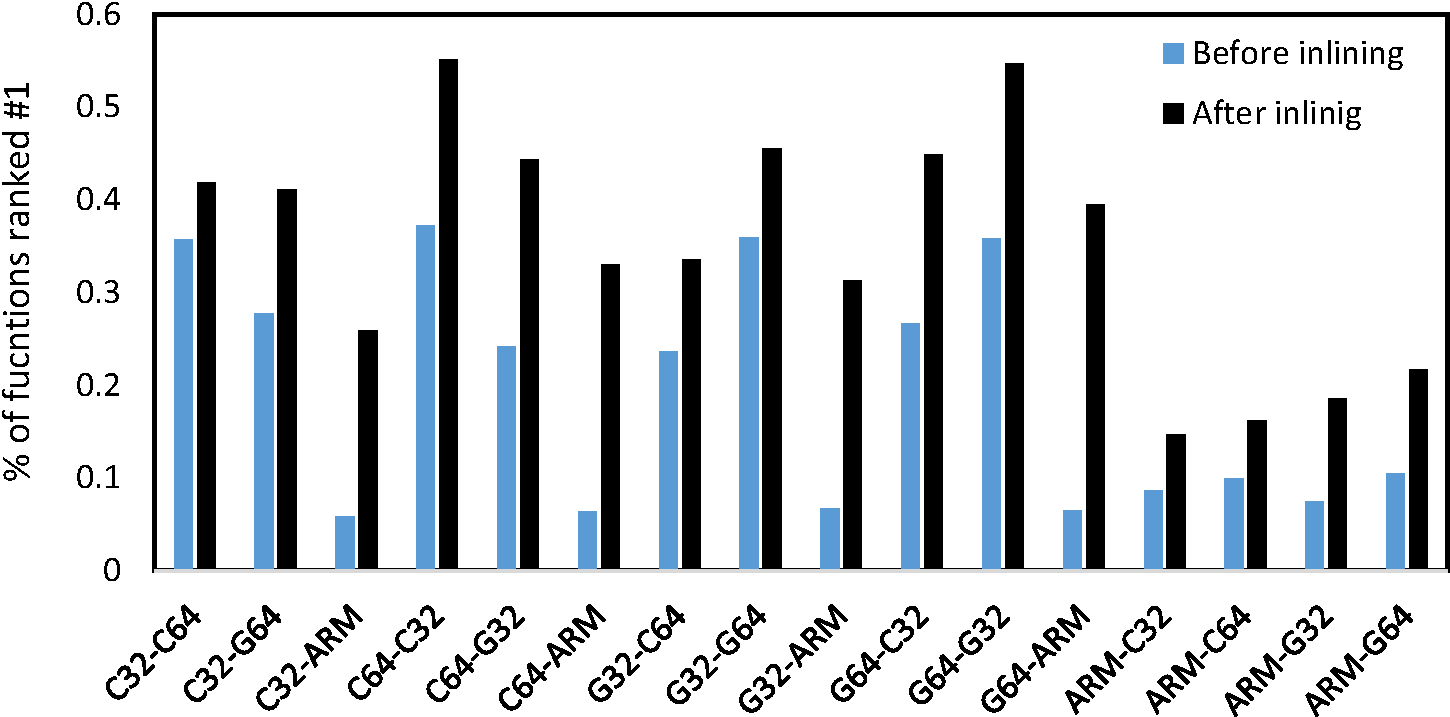
\includegraphics[height=4cm]{srj-figures/srj-cross-archi.pdf} %\vspace{-1mm}
\caption{In \tool, cross-architecture function matching before/after selective inlining using \texttt{coreutils} binaries. Here, \textbf{C} and \textbf{G} represent  compilers \texttt{clang} and \texttt{gcc}, respectively, and 32 and 64 denote x86 32bit and 64bit architectures. }
\label{fig:cross-archi}

\end{center}
\end{figure}


%\noindent\textbf{Cross-architecture analysis.}
%\textbf{Answer to RQ1.a: Cross-architecture analysis.}\label{sec:expe:rq1_a}
\subsubsection{\tool's Answer to RQ1}\label{sec:evaluation_rq1.1}
We conduct two experiments. First experiment is to match all functions in \texttt{coreutils} binaries compiled for one architecture (i.e., x86 32bit, x86 64bit and ARM) to the semantically equivalent functions in binaries compiled for another architecture. For example, binaries compiled for ARM are matched against the binaries compiled for x86 32bit and x86 64bit architectures, and \emph{vice versa}.  In all three architectures, the compilation uses \texttt{gcc} (v4.8.2) and \texttt{clang} (v3.0) with the optimization level \texttt{O2} (default settings in many Linux distributions).

Fig.~\ref{fig:cross-archi} summarizes the average results (before and after selective inlining) obtained for \texttt{coreutils} binaries, where we report the percentage of functions ranked one (i.e., best match).
%in the matching.
In the plot,  the bar \texttt{G64-G32} (after inlining) should be read as, when functions compiled, using \texttt{gcc}, for x86 64bit architecture are used as signature, around 55\% of the functions compiled, using \texttt{gcc}, for x86 32bit architecture achieve rank one. It is observed that when ARM binary functions are used as signatures, the overall results significantly degrade --- only 18\% of the functions are ranked one, compare to x86 32bit and 64bit architectures, where it is around 41\%.
%Table \ref{tab:cross-arch-with-behav} summarizes the results for 14 largest \texttt{coreutils} binaries (e.g., \texttt{cp}, \texttt{df}, $\ldots$) and the last row shows the averages for rest of the 89 binaries . It can be seen that on average 18\% of the functions in the largest 14 binaries are ranked 1, this increases to 30.4\% for rest of the binaries. Further, around 71\% of the large binaries are ranked within top 5 positions, where it is 82\% for other small binaries.
We also notice that matching(after inlining) between binaries compiled for ARM and x86 64bit  yields higher ranking compared to ARM and x86 32bit binaries. The rationale is that ARM and x86 64bit binaries are register intensive compared to x86 32bit binaries ---  in ARM and x86 64bit architectures, there are 16 general-purpose registers, and hence registers are used more frequently than used in x86 32bit binaries which have only 8.

%However, the \texttt{coreutils} binaries are relatively small with around 100-150 functions (on avg.) per binary. Hence, to compare the robustness of \tool in larger binaries with several thousand functions, we repeated the experiment with \texttt{BusyBox} (v1.21.1), where functions in x86 32bit, x86 62bit and ARM are matched against each other.
%From Table \ref{tab:x86_x64_box},
Considering the fact that \texttt{coreutils} binaries are relatively small with around 250 functions (on average) per binary, we conduct the second experiment using \texttt{BusyBox} (v1.21.1), which contains 2,410 functions.
%\xyx{Considering the relatively small size of functions (100-150) in \texttt{coreutils}, we conduct the same experiment on the second case \texttt{BusyBox} (v1.21.1) which contains 2410 functions.}
We observe that the obtained results are comparable with the results of \texttt{coreutils} binaries --- 41.3\% of the functions are best-match in \texttt{BusyBox}, while it is 35\% for \texttt{coreutils} binaries on average across 16 experiments shown in Fig.~\ref{fig:cross-archi}. This is an improvement of 27.5\% over the accuracy achieved by~\cite{DBLP:conf/sp/PewnyGGRH15} for \texttt{BusyBox}.
However, for top-10 match (i.e., ranking 1-10), \texttt{coreutils} binaries achieve better results than \texttt{BusyBox} (78.4\% vs. 67\%). This result might be due to function size of the binary --- in \texttt{BusyBox}, a function needs to be compared against on average 3,250 functions, and in \texttt{coreutils} binaries around 250  functions need to be compared. %This illustrates the robustness of \tool across architectures.\\

\begin{table}[t]
\scriptsize
\centering
\caption{Total no. of functions selectively inlined in \texttt{coreutils} binaries compiled using \texttt{gcc} and \texttt{clang} for ARM, x86 32bit and 64bit architectures. }
\label{cross-archi-inline}
\begin{tabular}{@{}llllll@{}}
\toprule
                                         & ARM                        & C64                        & G64                        & C32                        & G32                        \\ \midrule
\multicolumn{1}{l|}{Total functions}     & \multicolumn{1}{l|}{27,820} & \multicolumn{1}{l|}{23,782} & \multicolumn{1}{l|}{24,489} & \multicolumn{1}{l|}{24,002} & \multicolumn{1}{l|}{24,792} \\ \cmidrule(l){2-6}
%\multicolumn{1}{l|}{Candidate functions} & \multicolumn{1}{l|}{4251}  & \multicolumn{1}{l|}{2260}  & \multicolumn{1}{l|}{2671}  & \multicolumn{1}{l|}{2464}  & \multicolumn{1}{l|}{3295}  \\ \cmidrule(l){2-6}
\multicolumn{1}{l|}{Inlined functions}   & \multicolumn{1}{l|}{1,620}  & \multicolumn{1}{l|}{776}   & \multicolumn{1}{l|}{1,002}  & \multicolumn{1}{l|}{823}   & \multicolumn{1}{l|}{1,188}  \\ \bottomrule
\end{tabular}
\end{table}


\noindent\textbf{Impact of selective inlining.} As shown in Fig.~\ref{fig:cross-archi}, our selective inlining significantly improves the overall matching accuracy by 150\% on average. In particular, when ARM architecture is used as target, selective inlining improves the total matching accuracy on average by about 400\%. Table~\ref{cross-archi-inline} summarizes the total number of functions inlined for each architecture.  We notice that \texttt{coreutils} compiled for ARM contains more functions (27,820 across 103 binaries) than that compiled for x86 32bit (avg. 24,397) and x86 64bit (avg. 24,136). From the second row of Table~\ref{cross-archi-inline}, it can be seen that 61\% and 82\% more functions are selectively inlined by \tool in ARM than that in x86 32bit and 64bit architectures, respectively. In ARM binaries, the larger number of compiled functions suggests that compiler inlining does not happen as frequently as it does in the other two architectures.  Hence,   selective inlining is required to capture the complete semantics in binary analysis, which results in the improved matching accuracy.

\noindent\textbf{Summary.} On \texttt{coreutils} and \texttt{BusyBox} binaries, \tool achieves the best match (i.e., rank \#1) for 35\%-42\% of the functions on average, for cross-architecture analysis, and selective inlining improves the result by 150\% on average.

\subsubsection{\toolNew's Answer to RQ1}\label{sec:evaluation_rq1.2}

\begin{figure}[t]
\begin{center}%\vspace{-3mm}
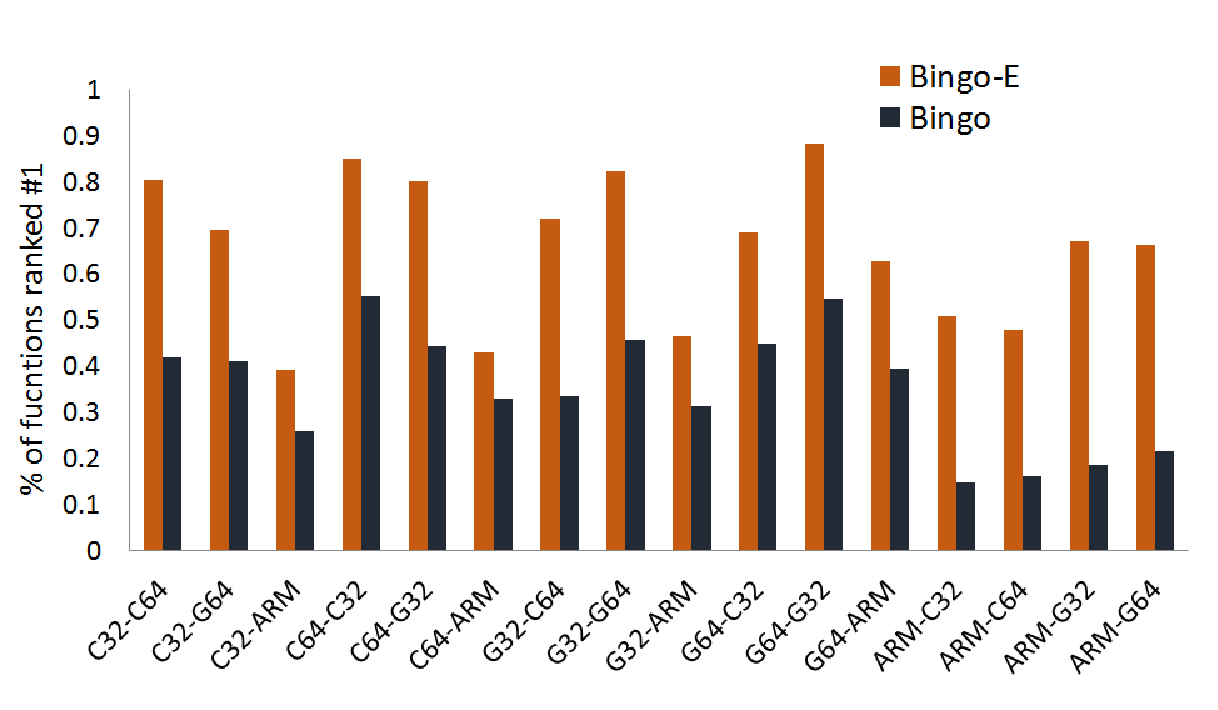
\includegraphics[height=5cm]{srj-figures/cross-archi-new.pdf} %\vspace{-1mm}
\caption{Cross-architecture function matching after selective inlining using \texttt{coreutils} binaries for \tool and \toolNew. Here, \textbf{C} and \textbf{G} represent  compilers \texttt{clang} and \texttt{gcc}, respectively, and 32 and 64 denote x86 32bit and 64bit architectures. }
\label{fig:cross-archi-new}
\end{center}
\end{figure}


For \toolNew, we also match the binary functions in \texttt{coreutils} binaries compiled for one architectures (i.e., x86 32bit, x86 64bit and ARM) to that for another. We use the two compilers \texttt{gcc} (v4.8.2) and \texttt{clang} (v3.0) with the optimization level \texttt{O2} (default settings in many Linux distributions). %Hence, the setup of the experiment is the same as that in \S~\ref{subsec:robut}.

Fig.~\ref{fig:cross-archi-new} shows the average results after selective inlining on \texttt{coreutils} binaries for \tool and \toolNew.
Note we only count the percentage of functions ranked 1st (i.e., best match in the case of mapping the binary functions from the same source code).
In Fig.~\ref{fig:cross-archi-new}, we list 16 possible scenarios of cross-architecture code matching.
For example, in the plot, the brown bar \texttt{G64-ARM}  denotes the result that 62.7\% of the functions (signatures) compiled by \texttt{gcc}  for  x86-64 are the best matches of those functions (targets) compiled by \texttt{gcc} for ARM architecture according to \toolNew.

Previously, we observed that in Fig.~\ref{fig:cross-archi} that when  binary functions compiled for ARM are used as signatures, the  matching results significantly degrade --- only 18\% of the functions are ranked 1st, based on the low-level semantic features in \tool. \xyx{The reason is that  I/O values of registers in \tool are not effective for cross-architecture matching.} Hence, in \toolNew, the newly added high-level semantic and structural features are complement to improve the matching accuracy. The results in Fig.~\ref{fig:cross-archi-new} prove the effectiveness of these new features. For most cases, the new features improve the matching accuracy by at least 50\%, compared to the results of \tool. Especially, in the cases of code for ARM as signatures (\texttt{ARM-C32}, \texttt{ARM-C64}, \texttt{ARM-G32}, \texttt{ARM-G64}), the improvement of best match rate is above 200\%. This indicates the ineffectiveness of low-level semantic features used by \tool for matching the code for ARM to the code for other architectures.


%Only in the cases of code for ARM as targets (\texttt{C32-ARM}, \texttt{C64-ARM} and \texttt{G32-ARM}), the improvement is less than 50\%.
\xyx{Currently, for \toolNew, we get more similar results for many cases --- the best match rate is within the range of  $70\% \sim 90\%$ for  the mapping from x86-32 to x86-64 (or the other way around), while the  best match rate drops to  $40\% \sim 60\%$ if the ARM code is used as signatures or targets. The rationale is that the BB structure of code for x86-32 or x86-64 is highly similar; even in code for ARM, the basic BB structure is also retained during the cross-architecture compilation.
Hence, the structural features and high-level semantic features are the effective complements, since the CFG structures and function call information are retained during the compilation (no matter we use \texttt{gcc}  or \texttt{clang}). We find that the high-level semantic features, if  they are available, are even more helpful than structural features. The reason is that after selective inlining the information on function call in binary code does not change with the compilation options of architecture.}

Another interesting observation is that the results for \toolNew are much more symmetric than the results of \tool. For example, the best match rate for \toolNew in \texttt{C64-ARM} and \texttt{ARM-C64} is 0.431 and 0.479, respectively. Hence, reversing signatures and targets does not affect as much as that in \tool. In contrast,  for \tool in \texttt{C64-ARM} and \texttt{ARM-C64} it is 0.33 and 0.162, respectively. The unsymmetrical results for \tool are due to the step of function model generation, in which $k$-tracelet is sampled and generated from the CFG. As applying graph isomorphism for CFG matching, the matching of CFG $g_1$ to $g_2$ does not mean the matching of $g_2$ to $g_1$ --- $g_1$ may be a sub-graph of $g_2$ and using $g_2$ as signatures leads to a similarity score lower than the similarity threshold. Similarly, in \tool, low level semantic features extracted from $k$-tracelet (i.e., sampled partial CFG) also have this issue of unsymmetrical results.

To mitigate this, the function similarity  (i.e., FDD in \S~\ref{sec:category:structralFea}) for 3D-CFG is defined to produce symmetrical results, according to Definition 3. In addition, the high-level semantic features (e.g., function call information) are retained in cross-architecture compilation. Hence, the results of \toolNew are more symmetrical than that of \tool.

%Nevertheless, when the ARM code is used as targets, the structural features are less effective than they are when the code for e x86-32 or x86-64  is targets. %\xyx{After a  scrutiny of the matching results, we observe that,  after the compilation of the source code, the code for ARM seems to have simpler BB structure than that for x86-32 or x86-64. Accord to the 3D-CFG features,  }
%Table \ref{tab:cross-arch-with-behav} summarizes the results for 14 largest \texttt{coreutils} binaries (e.g., \texttt{cp}, \texttt{df}, $\ldots$) and the last row shows the averages for rest of the 89 binaries . It can be seen that on average 18\% of the functions in the largest 14 binaries are ranked 1, this increases to 30.4\% for rest of the binaries. Further, around 71\% of the large binaries are ranked within top 5 positions, where it is 82\% for other small binaries.

%We also notice that matches (after inlining) between binaries compiled for ARM and x86 64bit  yield higher ranking compared to ARM and x86 32bit binaries. The rationale is that ARM and x86 64bit binaries are register intensive compared to x86 32bit binaries ---  in ARM and x86 64bit architectures, there are 16 general-purpose registers, and hence registers are used more frequently than used in x86 32bit binaries which have only 8.

\vspace{2mm}
\noindent\fbox{\parbox{1\linewidth}{In this experiment, on average, our approach significantly improves the accuracy of best match rate from 35.1\% (for \tool) to 65.6\% (for \toolNew) on \texttt{coreutils}.  For cross-architecture matching on the same code base, structural features and high-level semantic features are effective, being good complement to low-level semantic features. Further, \toolNew's results are more symmetrical than \tool's.}  }


%\begin{table}[ht]
%\caption{Percentage of functions ranked \#1 in intra-compiler (x86 64bit) comparison. Here, \textbf{G} and \textbf{G'} represent \texttt{gcc} v4.8.3 and v4.6 compilers, respectively.}
%\begin{minipage}{.5\linewidth}
%
%\scriptsize
%
%\label{my-label}
%\begin{tabular}{@{}lllll@{}}
%                        & G0                        & G1                        & G2                        & G3                        \\ \cmidrule(l){2-5}
%\multicolumn{1}{l|}{G'0} & \multicolumn{1}{l|}{0.45} & \multicolumn{1}{l|}{0.37} & \multicolumn{1}{l|}{0.41} & \multicolumn{1}{l|}{0.25} \\ \cmidrule(l){2-5}
%\multicolumn{1}{l|}{G'1} & \multicolumn{1}{l|}{0.37} & \multicolumn{1}{l|}{0.47} & \multicolumn{1}{l|}{0.51} & \multicolumn{1}{l|}{0.32} \\ \cmidrule(l){2-5}
%\multicolumn{1}{l|}{G'2} & \multicolumn{1}{l|}{0.47} & \multicolumn{1}{l|}{0.54} & \multicolumn{1}{l|}{0.57} & \multicolumn{1}{l|}{0.47} \\ \cmidrule(l){2-5}
%\multicolumn{1}{l|}{G'3} & \multicolumn{1}{l|}{0.37} & \multicolumn{1}{l|}{0.44} & \multicolumn{1}{l|}{0.52} & \multicolumn{1}{l|}{0.54} \\ \cmidrule(l){2-5}
%\end{tabular}
%\end{minipage}%
%\begin{minipage}{.5\linewidth}
%
%\scriptsize
%
%\label{my-label}
%\begin{tabular}{@{}lllll@{}}
%                        & G'0                        & G'1                        & G'2                        & G'3                        \\ \cmidrule(l){2-5}
%\multicolumn{1}{l|}{G0} & \multicolumn{1}{l|}{0.45} & \multicolumn{1}{l|}{0.36} & \multicolumn{1}{l|}{0.41} & \multicolumn{1}{l|}{0.34} \\ \cmidrule(l){2-5}
%\multicolumn{1}{l|}{G1} & \multicolumn{1}{l|}{0.39} & \multicolumn{1}{l|}{0.49} & \multicolumn{1}{l|}{0.52} & \multicolumn{1}{l|}{0.39} \\ \cmidrule(l){2-5}
%\multicolumn{1}{l|}{G2} & \multicolumn{1}{l|}{0.44} & \multicolumn{1}{l|}{0.55} & \multicolumn{1}{l|}{0.59} & \multicolumn{1}{l|}{0.53} \\ \cmidrule(l){2-5}
%\multicolumn{1}{l|}{G3} & \multicolumn{1}{l|}{0.3}  & \multicolumn{1}{l|}{0.39} & \multicolumn{1}{l|}{0.51} & \multicolumn{1}{l|}{0.51} \\ \cmidrule(l){2-5}
%\end{tabular}
%\end{minipage}%
%\end{table}


%\begin{table}[t]
%\scriptsize
%\centering
%\caption{Rankings (top 10 matches) obtained by \tool for 60 functions in \texttt{msvcrt} against \texttt{libc}}
%\label{tab:cross-os}
%\begin{tabular}{@{}lll@{}}
%\multicolumn{1}{c}{\textbf{Rank}}    & \multicolumn{1}{c}{\textbf{Library functions}}   & \#                       \\ \cmidrule(l){1-3}
%\multicolumn{1}{l|}{1}      & \multicolumn{1}{l|}{\parbox{6cm}{tolower, memset, wcschr, wcsncmp, toupper, memcmp, strspn, wcsrchr, memchr, strrch,r strchr}}                                                              & \multicolumn{1}{l}{11}  \\ \cmidrule(l){1-3}
%\multicolumn{1}{l|}{2-3}    & \multicolumn{1}{l|}{\parbox{6cm}{wcstoul, wcstol, strtoul, fopen, strncpy, strtol, itoa, wcscmp, wcsncat, itow, longjmp, strcspn, wcsncpy, labs, strpbrk, toupper, write, memcpy, memmove, tolower}} & \multicolumn{1}{l}{20} \\ \cmidrule(l){1-3}
%\multicolumn{1}{l|}{4-5}    & \multicolumn{1}{l|}{\parbox{6cm}{mbtowc, wcstombs, strcat, remove, mbstowcs, wctomb}}                                                                                                   & \multicolumn{1}{l}{6}  \\ \cmidrule(l){1-3}
%\multicolumn{1}{l|}{6-10}   & \multicolumn{1}{l|}{\parbox{6cm}{rename, strstr, wcspbrk, iswctype, strtok, wcscoll, strcoll, setlocale, qsort, wcsspn, swprintf, wcstod, strerrorr}}                                         & \multicolumn{1}{l}{13}  \\ \cmidrule(l){1-3}
%%\multicolumn{1}{l|}{11-20}  & \multicolumn{1}{l|}{\parbox{6cm}{strncat, raise, strtod, wcscspn, wcstok, atol}}                                                                                                        & \multicolumn{1}{l|}{6}  \\ \cmidrule(l){1-3}
%%\multicolumn{1}{l|}{21-50}  & \multicolumn{1}{l|}{perror, system, wcsxfrm}                                                                                                                           & \multicolumn{1}{l|}{3}   \\ \cmidrule(l){1-3}
%%\multicolumn{1}{l|}{51-100} & \multicolumn{1}{l|}{strxfrm}                                                                                                                                           & \multicolumn{1}{l|}{1}      \\ \cmidrule(l){1-3}
%\end{tabular}\vspace{-1mm}
%\end{table}

%\noindent\textbf{Cross-compiler analysis.}

\subsection{Answer to RQ2: Robustness in Cross-compiler Matching}\label{sec:evaluation_rq2}
\subsubsection{\tool's Answer to RQ2}

\textbf{Inter-compiler Matching.} Table~\ref{tab:cross-comp-inter} summarizes the results obtained by \tool for different compilers (\texttt{gcc} and \texttt{clang}) with various optimization levels (O0, O1, O2 and O3) for x86 32bit architecture.
Here, each row and column of the table represents the compiler (including the level of optimization) used to compile the signature and target functions, respectively.
%functions while each column denotes the compiler used to compile the target functions.
For example, the cell denoted by the second row and fifth column (\texttt{C1G0}) represents the result for which signature functions are compiled using \texttt{clang}  with optimization level \texttt{O1} and the target functions are compiled using \texttt{gcc} with  \texttt{O0}.
From the table, we observe that \tool is good, %in most cases (except when  \texttt{gcc\_O3} is used as a signature)
as 41.5\% of the functions achieve rank one (on average across all the experiments for binaries compiled for x86 32bit) while this increases to 84\% for top 10 matches, which is very promising. We observed similar behaviour in binaries compiled for x86 64bit architecture and due to space constraints, the results are reported in our tool webpage~\cite{bingo@fse2016}.% Further, we also report the individual results obtained by each of these 103 binaries (e.g., \texttt{ls}, \texttt{true}, and so on) in the \texttt{coretuils} suite, for every experiment, in~\cite{bingo@fse2016}.
%In addition, during cross-compiler analysis, if no optimization is used in either one of the side, the obtained rankings are relatively low compare to optimized binaries, this observation is inlined with~\cite{DBLP:conf/sp/PewnyGGRH15}.

Interestingly, we find that regardless of the compiler type, matches between the binaries that are compiled with high code optimization levels (i.e., \texttt{O2} and \texttt{O3}) yield better results than matches between binaries with no code optimization (i.e.,\texttt{O0}). That is, high code optimization levels lead to the similar binary code even with different compilers, whereas without optimization the  influence of the compiler in the binary is very evident. This observation is consistent with~\cite{DBLP:conf/sp/PewnyGGRH15}. Further, within one compiler type (e.g., \texttt{gcc}), the matching accuracy achieved by optimization level \texttt{O2}, across all other compiler types and optimization levels, is always better or consistent with the results obtained by \texttt{O3} (relevant rows are shaded in light gray in Table~\ref{tab:cross-comp-inter}). This behaviour is observed in x86 64bit architecture too.


\noindent\textbf{Intra-compiler Matching.} In addition, we also conduct the experiments across different versions of the same compiler (\texttt{gcc} v4.8.3 vs. \texttt{gcc} v4.6) and the results (for x86 32bit architecture) are summarized in Table~\ref{tab:cross-comp-intra}.
%The observations are pretty similar to the inter-compiler analysis, where the comparisons against optimized code, in general, achieve better accuracy while the comparisons against unoptimized code weakens the matching accuracy.
%Interestingly,  it is observed that when functions compiled with optimization level \texttt{O1} are used as signatures, functions compiled with optimization level \texttt{O2} yield better accuracy, except when \texttt{gcc} v4.8.3 is used to compile the signature binaries for x86 32bit architecture.
%For all other cases,
As expected, the highest accuracy is achieved when the signature and target functions are of the same optimization level, except when the signature functions are compiled with optimization level \texttt{O1}, where on such occasions, target functions compiled with optimization level \texttt{O2} yield better accuracy. The best results obtained for each signature binary is highlighted in light gray in Table~\ref{tab:cross-comp-intra}.
Further, we also observe that the overall accuracy for intra-compiler analysis (42.7\%) is slightly better than the inter-compiler analysis (41.5\%). %where 43.6\% (overall average) of the functions achieved rank one in intra-compiler analysis, a 5.5\% improvement.
Finally, in intra-compiler analysis, around 76.3\% functions ranked within top 5 positions, whereas it is only 68.5\% for inter-compiler analysis, an 11.8\% improvement. Details on the results of intra-compiler analysis for x86 64bit architecture are reported in~\cite{bingo@fse2016}.
%within same compilers, better ranks are achieved when the functions are matched from optimization level O3 to O0 (i.e., highest to no optimization) and the worst ranks are achieved when the matching is inverted, i.e., from O0 to O3. This could be attributed to the fact that in O3 the compiler merges as many functions as possible, using function inlining, and makes the functions very compact. Hence, for one function in O3 there may be many semantically similar functions in O0, where there is no optimization at all (i.e.,\textit{ 1-to-n} matching). However, on the other hand, for several functions in O0 there will be only one function in O3 which may be semantically less similar to all of them individually (i.e., \textit{n-to-1} matching). This behavior is not particular to certain compiler as its observed both in \texttt{gcc} and \texttt{clang} compilers.

\noindent\textbf{Impact of selective inlining.}  We observe that selective inlining improves the average matching accuracy by around 140\% for cross-compiler analysis. Many functions are inlined when the binaries are compiled with the optimization level \texttt{O0} compared to \texttt{O3}. In particular, 1,473 functions (on average across \texttt{gcc} and \texttt{clang}) are inlined in for optimization level \texttt{O0}, whereas, it is only 831 for \texttt{O3}.

\noindent\textbf{Summary.} %On \texttt{coreutils} and \texttt{BusyBox} binaries, \tool achieves the best match (i.e., rank \#1) for 35\%-42\% of the functions on average, for cross-architecture analysis, and selective inlining improves the result by 150\% on average.
For different types and versions of compiler, in most cases, \tool attains the best match for around 42\% of the functions, and top-5 match for around 72\% of the functions on average.

\begin{table}[t]
\scriptsize
\centering
\caption{In \tool, percentage of functions ranked \#1 in inter-compiler (x86 32bit) comparison for \texttt{coreutils}. Here, \textbf{C} and \textbf{G} represent \texttt{clang} and \texttt{gcc} compilers, respectively and 0-3 represents optimization O0-O3. }
\label{tab:cross-comp-inter}
\begin{tabular}{@{}lllllllll@{}}
\textbf{} & \textbf{C0} & \textbf{C1} & \textbf{C2} & \textbf{C3} & \textbf{G0} & \textbf{G1} & \textbf{G2} & \textbf{G3} \\ \cmidrule(l){2-9}
\multicolumn{1}{l|}{\textbf{C0}} & \multicolumn{1}{c|}{-} & \multicolumn{1}{l|}{0.402} & \multicolumn{1}{l|}{0.373} & \multicolumn{1}{l|}{0.372} & \multicolumn{1}{l|}{0.371} & \multicolumn{1}{l|}{0.4} & \multicolumn{1}{l|}{0.451} & \multicolumn{1}{l|}{0.332} \\ \cmidrule(l){2-9}
\multicolumn{1}{l|}{\textbf{C1}} & \multicolumn{1}{l|}{0.392} & \multicolumn{1}{c|}{-} & \multicolumn{1}{l|}{0.456} & \multicolumn{1}{l|}{0.455} & \multicolumn{1}{l|}{0.396} & \multicolumn{1}{l|}{0.429} & \multicolumn{1}{l|}{0.503} & \multicolumn{1}{l|}{0.388} \\ \cmidrule(l){2-9}
\multicolumn{1}{l|}{\textbf{C2}} & \multicolumn{1}{l|}{\cellcolor[HTML]{EFEFEF}0.345} & \multicolumn{1}{l|}{\cellcolor[HTML]{EFEFEF}0.426} & \multicolumn{1}{c|}{\cellcolor[HTML]{EFEFEF}-} & \multicolumn{1}{l|}{\cellcolor[HTML]{EFEFEF}0.576} & \multicolumn{1}{l|}{\cellcolor[HTML]{EFEFEF}0.344} & \multicolumn{1}{l|}{\cellcolor[HTML]{EFEFEF}0.411} & \multicolumn{1}{l|}{\cellcolor[HTML]{EFEFEF}0.488} & \multicolumn{1}{l|}{\cellcolor[HTML]{EFEFEF}0.478} \\ \cmidrule(l){2-9}
\multicolumn{1}{l|}{\textbf{C3}} & \multicolumn{1}{l|}{0.344} & \multicolumn{1}{l|}{0.425} & \multicolumn{1}{l|}{0.575} & \multicolumn{1}{c|}{-} & \multicolumn{1}{l|}{0.343} & \multicolumn{1}{l|}{0.41} & \multicolumn{1}{l|}{0.488} & \multicolumn{1}{l|}{0.477} \\ \cmidrule(l){2-9}
\multicolumn{1}{l|}{\textbf{G0}} & \multicolumn{1}{l|}{0.344} & \multicolumn{1}{l|}{0.354} & \multicolumn{1}{l|}{0.334} & \multicolumn{1}{l|}{0.333} & \multicolumn{1}{c|}{-} & \multicolumn{1}{l|}{0.374} & \multicolumn{1}{l|}{0.398} & \multicolumn{1}{l|}{0.302} \\ \cmidrule(l){2-9}
\multicolumn{1}{l|}{\textbf{G1}} & \multicolumn{1}{l|}{0.37} & \multicolumn{1}{l|}{0.409} & \multicolumn{1}{l|}{0.41} & \multicolumn{1}{l|}{0.409} & \multicolumn{1}{l|}{0.376} & \multicolumn{1}{c|}{-} & \multicolumn{1}{l|}{0.517} & \multicolumn{1}{l|}{0.395} \\ \cmidrule(l){2-9}
\multicolumn{1}{l|}{\textbf{G2}} & \multicolumn{1}{l|}{\cellcolor[HTML]{EFEFEF}0.412} & \multicolumn{1}{l|}{\cellcolor[HTML]{EFEFEF}0.462} & \multicolumn{1}{l|}{\cellcolor[HTML]{EFEFEF}0.474} & \multicolumn{1}{l|}{\cellcolor[HTML]{EFEFEF}0.473} & \multicolumn{1}{l|}{\cellcolor[HTML]{EFEFEF}0.428} & \multicolumn{1}{l|}{\cellcolor[HTML]{EFEFEF}0.514} & \multicolumn{1}{c|}{\cellcolor[HTML]{EFEFEF}-} & \multicolumn{1}{l|}{\cellcolor[HTML]{EFEFEF}0.48} \\ \cmidrule(l){2-9}
\multicolumn{1}{l|}{\textbf{G3}} & \multicolumn{1}{l|}{0.326} & \multicolumn{1}{l|}{0.372} & \multicolumn{1}{l|}{0.438} & \multicolumn{1}{l|}{0.439} & \multicolumn{1}{l|}{0.331} & \multicolumn{1}{l|}{0.42} & \multicolumn{1}{l|}{0.5} & \multicolumn{1}{c|}{-} \\ \cmidrule(l){2-9}
\end{tabular}
\end{table}



\begin{table}[t]
%\vspace{5mm}
\caption{In \tool, percentage of functions ranked \#1 in intra-compiler (x86 32bit) comparison for \texttt{coreutils}. Here, \textbf{G} and \textbf{G'} represent \texttt{gcc} v4.8.3 and v4.6 compilers, respectively.}
\label{tab:cross-comp-intra}
\begin{minipage}{.5\linewidth}
\scriptsize
\begin{tabular}{@{}lllll@{}}
                        & G0                        & G1                        & G2                        & G3                        \\ \cmidrule(l){2-5}
\multicolumn{1}{l|}{G'0} & \multicolumn{1}{l|}{\cellcolor[HTML]{EFEFEF}0.43} & \multicolumn{1}{l|}{0.36} & \multicolumn{1}{l|}{0.36} & \multicolumn{1}{l|}{0.27} \\ \cmidrule(l){2-5}
\multicolumn{1}{l|}{G'1} & \multicolumn{1}{l|}{0.37} & \multicolumn{1}{l|}{0.46} & \multicolumn{1}{l|}{\cellcolor[HTML]{EFEFEF}0.48} & \multicolumn{1}{l|}{0.36} \\ \cmidrule(l){2-5}
\multicolumn{1}{l|}{G'2} & \multicolumn{1}{l|}{0.4}  & \multicolumn{1}{l|}{0.44} & \multicolumn{1}{l|}{\cellcolor[HTML]{EFEFEF}0.52} & \multicolumn{1}{l|}{0.41} \\ \cmidrule(l){2-5}
\multicolumn{1}{l|}{G'3} & \multicolumn{1}{l|}{0.4}  & \multicolumn{1}{l|}{0.44} & \multicolumn{1}{l|}{0.49} & \multicolumn{1}{l|}{\cellcolor[HTML]{EFEFEF}0.49} \\ \cmidrule(l){2-5}
\end{tabular}
\end{minipage}%
\begin{minipage}{.5\linewidth}

\scriptsize

\begin{tabular}{@{}lllll@{}}
                        & G'0                        & G'1                        & G'2                        & G'3                        \\ \cmidrule(l){2-5}
\multicolumn{1}{l|}{G0} & \multicolumn{1}{l|}{\cellcolor[HTML]{EFEFEF}0.44} & \multicolumn{1}{l|}{0.4}  & \multicolumn{1}{l|}{0.41} & \multicolumn{1}{l|}{0.42} \\ \cmidrule(l){2-5}
\multicolumn{1}{l|}{G1} & \multicolumn{1}{l|}{0.38} & \multicolumn{1}{l|}{0.47} & \multicolumn{1}{l|}{\cellcolor[HTML]{EFEFEF}0.48} & \multicolumn{1}{l|}{0.45} \\ \cmidrule(l){2-5}
\multicolumn{1}{l|}{G2} & \multicolumn{1}{l|}{0.4}  & \multicolumn{1}{l|}{0.49} & \multicolumn{1}{l|}{\cellcolor[HTML]{EFEFEF}0.52} & \multicolumn{1}{l|}{0.5}  \\ \cmidrule(l){2-5}
\multicolumn{1}{l|}{G3} & \multicolumn{1}{l|}{0.32} & \multicolumn{1}{l|}{0.39} & \multicolumn{1}{l|}{0.43} & \multicolumn{1}{l|}{\cellcolor[HTML]{EFEFEF}0.52} \\ \cmidrule(l){2-5}
\end{tabular}
\end{minipage}\vspace{0mm}%
\end{table}

\subsubsection{\toolNew's answer to RQ2}

\textbf{Inter-compiler Matching.} Still using \texttt{coreutils} binaries, Table \ref{tab:new_cross-comp-inter} summarizes the results obtained by \toolNew for different compilers (gcc and clang) with various optimization levels (O0, O1, O2 and O3) on  \texttt{coreutils} for x86 32bit architecture. The row represents the optimization level of signature functions and the column represents that of target functions. We observe that the best results are usually achieved when O1 or O2 is adopted. The worst results (below 80\%) are achieved when O3 is used, no matter for \texttt{gcc} or \texttt{clang}. Even C2-to-G1 or G2-to-C1 can achieve an accuracy above 88\%. Hence, for cross-compiler matching, we find the impact of compiler differences matters less than that of the optimization levels.

\vspace{2mm}
\noindent\fbox{\parbox{1\linewidth}{In this experiment, \toolNew (best-match rate ranging from 70.1\% to 99.7\% in Table \ref{tab:new_cross-comp-inter}) exhibits significant improvement over \tool (best-match rate ranging from 32\% to 58\% in Table \ref{tab:cross-comp-inter}) for cross-compiler analysis. The improvement is attributed to the use of features of BB structure and high-level semantics, as BB structure can be retained for different compilers under the same or similar optimization levels.}}

\vspace{2mm}

\textbf{Intra-compiler Matching.} We also conduct intra-compiler matching for \toolNew. Table~\ref{tab:new_cross-comp-intra} summarizes the searching results obtained by \toolNew for differen versions of the compiler \texttt{gcc} with various optimization levels (O0, O1, O2 and O3) for x86 32bit architecture. Here, each row and column of the table represents the compiler (including the level of optimization) used to compile the signature and target functions, respectively. For example, for the cell at row G'0 and column G0 in the left part of Table~\ref{tab:new_cross-comp-intra}, the value 0.91 means that 91\% of functions successfully match if we use the version compiled by G'0 as signature and use the function compiled  by G0 as target. It can be observed that usually the best-match results are achieved when the signature and target functions are combined by the same optimization level (O0-O2, except O3). The reasons lie that \toolNew adopts the structural and high-level semantic features for intra and cross compiler matching. When the same optimization level (except O3) is used for signature and target functions, the structural information is well-retained. However, when O3 is used, the structure of the binary is so over-optimized that less information is retained for structural matching. The two over-optimized program may have less structural similarity in G'3-to-G3 or G3-to-G'3 matching.

\vspace{2mm}
\noindent\fbox{\parbox{1\linewidth}{In the experiment, the results of \toolNew (best-match rate ranging from 70\% to 98\% in Table \ref{tab:new_cross-comp-intra}) are significantly better than the results of \tool (best-match rate ranging from 27\% to 52\% in  Table \ref{tab:cross-comp-intra}). For the same code base with intra-compiler matching, the structural and high-level semantic features are more effective than the low-level semantic features, relying on the retained structural information. }}



\begin{table}[t]
\scriptsize
\centering
\caption{In \toolNew, percentage of functions ranked \#1 in inter-compiler (x86 32bit) comparison for \texttt{coreutils}. Here, \textbf{C} and \textbf{G} represent \texttt{clang} and \texttt{gcc} compilers, respectively and 0-3 represents optimization O0-O3. }
\label{tab:new_cross-comp-inter}
\begin{tabular}{@{}lllllllll@{}}
\textbf{} & \textbf{C0} & \textbf{C1} & \textbf{C2} & \textbf{C3} & \textbf{G0} & \textbf{G1} & \textbf{G2} & \textbf{G3} \\ \cmidrule(l){2-9}
\multicolumn{1}{l|}{\textbf{C0}} & \multicolumn{1}{c|}{-} & \multicolumn{1}{l|}{0.865} & \multicolumn{1}{l|}{0.791} & \multicolumn{1}{l|}{0.785} & \multicolumn{1}{l|}{0.799} & \multicolumn{1}{l|}{0.840} & \multicolumn{1}{l|}{0.836} & \multicolumn{1}{l|}{0.701} \\ \cmidrule(l){2-9}
\multicolumn{1}{l|}{\textbf{C1}} & \multicolumn{1}{l|}{0.840} & \multicolumn{1}{c|}{-} & \multicolumn{1}{l|}{0.838} & \multicolumn{1}{l|}{0.833} & \multicolumn{1}{l|}{0.891} & \multicolumn{1}{l|}{0.913} & \multicolumn{1}{l|}{0.887} & \multicolumn{1}{l|}{0.756} \\ \cmidrule(l){2-9}
\multicolumn{1}{l|}{\textbf{C2}} & \multicolumn{1}{l|}{\cellcolor[HTML]{EFEFEF}0.814} & \multicolumn{1}{l|}{\cellcolor[HTML]{EFEFEF}0.889} & \multicolumn{1}{c|}{\cellcolor[HTML]{EFEFEF}-} & \multicolumn{1}{l|}{\cellcolor[HTML]{EFEFEF}0.996} & \multicolumn{1}{l|}{\cellcolor[HTML]{EFEFEF}0.862} & \multicolumn{1}{l|}{\cellcolor[HTML]{EFEFEF}0.926} & \multicolumn{1}{l|}{\cellcolor[HTML]{EFEFEF}0.858} & \multicolumn{1}{l|}{\cellcolor[HTML]{EFEFEF}0.757} \\ \cmidrule(l){2-9}
\multicolumn{1}{l|}{\textbf{C3}} & \multicolumn{1}{l|}{0.809} & \multicolumn{1}{l|}{0.885} & \multicolumn{1}{l|}{0.997} & \multicolumn{1}{c|}{-} & \multicolumn{1}{l|}{0.857} & \multicolumn{1}{l|}{0.924} & \multicolumn{1}{l|}{0.855} & \multicolumn{1}{l|}{0.759} \\ \cmidrule(l){2-9}
\multicolumn{1}{l|}{\textbf{G0}} & \multicolumn{1}{l|}{0.801} & \multicolumn{1}{l|}{0.888} & \multicolumn{1}{l|}{0.853} & \multicolumn{1}{l|}{0.846} & \multicolumn{1}{c|}{-} & \multicolumn{1}{l|}{0.884} & \multicolumn{1}{l|}{0.856} & \multicolumn{1}{l|}{0.754} \\ \cmidrule(l){2-9}
\multicolumn{1}{l|}{\textbf{G1}} & \multicolumn{1}{l|}{0.786} & \multicolumn{1}{l|}{0.878} & \multicolumn{1}{l|}{0.857} & \multicolumn{1}{l|}{0.852} & \multicolumn{1}{l|}{0.850} & \multicolumn{1}{c|}{-} & \multicolumn{1}{l|}{0.928} & \multicolumn{1}{l|}{0.857} \\ \cmidrule(l){2-9}
\multicolumn{1}{l|}{\textbf{G2}} & \multicolumn{1}{l|}{\cellcolor[HTML]{EFEFEF}0.806} & \multicolumn{1}{l|}{\cellcolor[HTML]{EFEFEF}0.882} & \multicolumn{1}{l|}{\cellcolor[HTML]{EFEFEF}0.814} & \multicolumn{1}{l|}{\cellcolor[HTML]{EFEFEF}0.808} & \multicolumn{1}{l|}{\cellcolor[HTML]{EFEFEF}0.848} & \multicolumn{1}{l|}{\cellcolor[HTML]{EFEFEF}0.963} & \multicolumn{1}{c|}{\cellcolor[HTML]{EFEFEF}-} & \multicolumn{1}{l|}{\cellcolor[HTML]{EFEFEF}0.732} \\ \cmidrule(l){2-9}
\multicolumn{1}{l|}{\textbf{G3}} & \multicolumn{1}{l|}{0.732} & \multicolumn{1}{l|}{0.773} & \multicolumn{1}{l|}{0.754} & \multicolumn{1}{l|}{0.753} & \multicolumn{1}{l|}{0.770} & \multicolumn{1}{l|}{0.863} & \multicolumn{1}{l|}{0.751} & \multicolumn{1}{c|}{-} \\ \cmidrule(l){2-9}
\end{tabular}
\end{table}


\begin{table}[t]
%\vspace{5mm}
\caption{In \toolNew, percentage of functions ranked \#1 in intra-compiler (x86 32bit) comparison for \texttt{coreutils}. Here, \textbf{G} and \textbf{G'} represent \texttt{gcc} v4.8.3 and v4.6 compilers, respectively.}
\label{tab:new_cross-comp-intra}
\begin{minipage}{.5\linewidth}
\scriptsize
\begin{tabular}{@{}lllll@{}}
                        & G0                        & G1                        & G2                        & G3                        \\ \cmidrule(l){2-5}
\multicolumn{1}{l|}{G'0} & \multicolumn{1}{l|}{\cellcolor[HTML]{EFEFEF}0.91} & \multicolumn{1}{l|}{0.86} & \multicolumn{1}{l|}{0.80} & \multicolumn{1}{l|}{0.70} \\ \cmidrule(l){2-5}
\multicolumn{1}{l|}{G'1} & \multicolumn{1}{l|}{0.86} & \multicolumn{1}{l|}{\cellcolor[HTML]{EFEFEF}0.97} & \multicolumn{1}{l|}{0.88} & \multicolumn{1}{l|}{0.82} \\ \cmidrule(l){2-5}
\multicolumn{1}{l|}{G'2} & \multicolumn{1}{l|}{0.85}  & \multicolumn{1}{l|}{0.94} & \multicolumn{1}{l|}{\cellcolor[HTML]{EFEFEF}0.97} & \multicolumn{1}{l|}{0.76} \\ \cmidrule(l){2-5}
\multicolumn{1}{l|}{G'3} & \multicolumn{1}{l|}{0.79}  & \multicolumn{1}{l|}{0.88} & \multicolumn{1}{l|}{\cellcolor[HTML]{EFEFEF}0.89} & \multicolumn{1}{l|}{0.75} \\ \cmidrule(l){2-5}
\end{tabular}
\end{minipage}%
\begin{minipage}{.5\linewidth}

\scriptsize

\begin{tabular}{@{}lllll@{}}
                        & G'0                        & G'1                        & G'2                        & G'3                        \\ \cmidrule(l){2-5}
\multicolumn{1}{l|}{G0} & \multicolumn{1}{l|}{\cellcolor[HTML]{EFEFEF}0.98} & \multicolumn{1}{l|}{0.88}  & \multicolumn{1}{l|}{0.84} & \multicolumn{1}{l|}{0.76} \\ \cmidrule(l){2-5}
\multicolumn{1}{l|}{G1} & \multicolumn{1}{l|}{0.84} & \multicolumn{1}{l|}{\cellcolor[HTML]{EFEFEF}0.94} & \multicolumn{1}{l|}{0.90} & \multicolumn{1}{l|}{0.84} \\ \cmidrule(l){2-5}
\multicolumn{1}{l|}{G2} & \multicolumn{1}{l|}{0.80}  & \multicolumn{1}{l|}{0.92} & \multicolumn{1}{l|}{\cellcolor[HTML]{EFEFEF}0.97} & \multicolumn{1}{l|}{0.81}  \\ \cmidrule(l){2-5}
\multicolumn{1}{l|}{G3} & \multicolumn{1}{l|}{0.72} & \multicolumn{1}{l|}{\cellcolor[HTML]{EFEFEF}0.83} & \multicolumn{1}{l|}{0.78} & \multicolumn{1}{l|}{0.74} \\ \cmidrule(l){2-5}
\end{tabular}
\end{minipage}\vspace{0mm}%
\end{table}



%\subsubsection{Robustness of \tool across compilers and code optimizations}
%\subsubsection{Answer to RQ2}





%\begin{table}[t]
%\scriptsize
%\centering
%\caption{Percentage of functions ranked \#1 in inter-compiler (x86 32bit) comparison. Here, \textbf{C} and \textbf{G} represent \texttt{clang} and \texttt{gcc} compilers, respectively and 0-3 represents optimization O0-O3. }
%\label{tab:cross-comp-inter}
%\begin{tabular}{@{}lllllllll@{}}
%\textbf{} & \textbf{C0} & \textbf{C1} & \textbf{C2} & \textbf{C3} & \textbf{G0} & \textbf{G1} & \textbf{G2} & \textbf{G3} \\ \cmidrule(l){2-9}
%\multicolumn{1}{l|}{\textbf{C0}} & \multicolumn{1}{c|}{-} & \multicolumn{1}{l|}{0.402} & \multicolumn{1}{l|}{0.373} & \multicolumn{1}{l|}{0.372} & \multicolumn{1}{l|}{0.371} & \multicolumn{1}{l|}{0.4} & \multicolumn{1}{l|}{0.451} & \multicolumn{1}{l|}{0.332} \\ \cmidrule(l){2-9}
%\multicolumn{1}{l|}{\textbf{C1}} & \multicolumn{1}{l|}{0.392} & \multicolumn{1}{c|}{-} & \multicolumn{1}{l|}{0.456} & \multicolumn{1}{l|}{0.455} & \multicolumn{1}{l|}{0.396} & \multicolumn{1}{l|}{0.429} & \multicolumn{1}{l|}{0.503} & \multicolumn{1}{l|}{0.388} \\ \cmidrule(l){2-9}
%\multicolumn{1}{l|}{\textbf{C2}} & \multicolumn{1}{l|}{\cellcolor[HTML]{EFEFEF}0.345} & \multicolumn{1}{l|}{\cellcolor[HTML]{EFEFEF}0.426} & \multicolumn{1}{c|}{\cellcolor[HTML]{EFEFEF}-} & \multicolumn{1}{l|}{\cellcolor[HTML]{EFEFEF}0.576} & \multicolumn{1}{l|}{\cellcolor[HTML]{EFEFEF}0.344} & \multicolumn{1}{l|}{\cellcolor[HTML]{EFEFEF}0.411} & \multicolumn{1}{l|}{\cellcolor[HTML]{EFEFEF}0.488} & \multicolumn{1}{l|}{\cellcolor[HTML]{EFEFEF}0.478} \\ \cmidrule(l){2-9}
%\multicolumn{1}{l|}{\textbf{C3}} & \multicolumn{1}{l|}{0.344} & \multicolumn{1}{l|}{0.425} & \multicolumn{1}{l|}{0.575} & \multicolumn{1}{c|}{-} & \multicolumn{1}{l|}{0.343} & \multicolumn{1}{l|}{0.41} & \multicolumn{1}{l|}{0.488} & \multicolumn{1}{l|}{0.477} \\ \cmidrule(l){2-9}
%\multicolumn{1}{l|}{\textbf{G0}} & \multicolumn{1}{l|}{0.344} & \multicolumn{1}{l|}{0.354} & \multicolumn{1}{l|}{0.334} & \multicolumn{1}{l|}{0.333} & \multicolumn{1}{c|}{-} & \multicolumn{1}{l|}{0.374} & \multicolumn{1}{l|}{0.398} & \multicolumn{1}{l|}{0.302} \\ \cmidrule(l){2-9}
%\multicolumn{1}{l|}{\textbf{G1}} & \multicolumn{1}{l|}{0.37} & \multicolumn{1}{l|}{0.409} & \multicolumn{1}{l|}{0.41} & \multicolumn{1}{l|}{0.409} & \multicolumn{1}{l|}{0.376} & \multicolumn{1}{c|}{-} & \multicolumn{1}{l|}{0.517} & \multicolumn{1}{l|}{0.395} \\ \cmidrule(l){2-9}
%\multicolumn{1}{l|}{\textbf{G2}} & \multicolumn{1}{l|}{\cellcolor[HTML]{EFEFEF}0.412} & \multicolumn{1}{l|}{\cellcolor[HTML]{EFEFEF}0.462} & \multicolumn{1}{l|}{\cellcolor[HTML]{EFEFEF}0.474} & \multicolumn{1}{l|}{\cellcolor[HTML]{EFEFEF}0.473} & \multicolumn{1}{l|}{\cellcolor[HTML]{EFEFEF}0.428} & \multicolumn{1}{l|}{\cellcolor[HTML]{EFEFEF}0.514} & \multicolumn{1}{c|}{\cellcolor[HTML]{EFEFEF}-} & \multicolumn{1}{l|}{\cellcolor[HTML]{EFEFEF}0.48} \\ \cmidrule(l){2-9}
%\multicolumn{1}{l|}{\textbf{G3}} & \multicolumn{1}{l|}{0.326} & \multicolumn{1}{l|}{0.372} & \multicolumn{1}{l|}{0.438} & \multicolumn{1}{l|}{0.439} & \multicolumn{1}{l|}{0.331} & \multicolumn{1}{l|}{0.42} & \multicolumn{1}{l|}{0.5} & \multicolumn{1}{c|}{-} \\ \cmidrule(l){2-9}
%\end{tabular}
%\end{table}

%\begin{table}[ht]
%\scriptsize
%\centering
%\caption{Percentage of functions ranked \#1 in inter-compiler (x86 64bit) comparison. }
%\label{my-label}
%\begin{tabular}{@{}lllllllll@{}}
%                        & C0                                                 & C1                                                 & C2                                                 & C3                                                 & G0                                                & G1                                                 & G2                                                 & G3                                                 \\ \cmidrule(l){2-9}
%\multicolumn{1}{l|}{C0} & \multicolumn{1}{c|}{\cellcolor[HTML]{EFEFEF}-}     & \multicolumn{1}{l|}{\cellcolor[HTML]{EFEFEF}0.36}  & \multicolumn{1}{l|}{\cellcolor[HTML]{EFEFEF}0.307} & \multicolumn{1}{l|}{\cellcolor[HTML]{EFEFEF}0.305} & \multicolumn{1}{l|}{\cellcolor[HTML]{EFEFEF}0.36} & \multicolumn{1}{l|}{\cellcolor[HTML]{EFEFEF}0.329} & \multicolumn{1}{l|}{\cellcolor[HTML]{EFEFEF}0.388} & \multicolumn{1}{l|}{\cellcolor[HTML]{EFEFEF}0.265} \\ \cmidrule(l){2-9}
%\multicolumn{1}{l|}{C1} & \multicolumn{1}{l|}{0.473}                         & \multicolumn{1}{c|}{-}                             & \multicolumn{1}{l|}{0.506}                         & \multicolumn{1}{l|}{0.504}                         & \multicolumn{1}{l|}{0.481}                        & \multicolumn{1}{l|}{0.501}                         & \multicolumn{1}{l|}{0.54}                          & \multicolumn{1}{l|}{0.429}                         \\ \cmidrule(l){2-9}
%\multicolumn{1}{l|}{C2} & \multicolumn{1}{l|}{0.356}                         & \multicolumn{1}{l|}{0.468}                         & \multicolumn{1}{c|}{-}                             & \multicolumn{1}{l|}{0.561}                         & \multicolumn{1}{l|}{0.368}                        & \multicolumn{1}{l|}{0.414}                         & \multicolumn{1}{l|}{0.518}                         & \multicolumn{1}{l|}{0.425}                         \\ \cmidrule(l){2-9}
%\multicolumn{1}{l|}{C3} & \multicolumn{1}{l|}{0.354}                         & \multicolumn{1}{l|}{0.466}                         & \multicolumn{1}{l|}{0.56}                          & \multicolumn{1}{c|}{-}                             & \multicolumn{1}{l|}{0.368}                        & \multicolumn{1}{l|}{0.413}                         & \multicolumn{1}{l|}{0.517}                         & \multicolumn{1}{l|}{0.425}                         \\ \cmidrule(l){2-9}
%\multicolumn{1}{l|}{G0} & \multicolumn{1}{l|}{\cellcolor[HTML]{EFEFEF}0.364} & \multicolumn{1}{l|}{\cellcolor[HTML]{EFEFEF}0.364} & \multicolumn{1}{l|}{\cellcolor[HTML]{EFEFEF}0.309} & \multicolumn{1}{l|}{\cellcolor[HTML]{EFEFEF}0.307} & \multicolumn{1}{c|}{\cellcolor[HTML]{EFEFEF}-}    & \multicolumn{1}{l|}{\cellcolor[HTML]{EFEFEF}0.349} & \multicolumn{1}{l|}{\cellcolor[HTML]{EFEFEF}0.41}  & \multicolumn{1}{l|}{\cellcolor[HTML]{EFEFEF}0.257} \\ \cmidrule(l){2-9}
%\multicolumn{1}{l|}{G1} & \multicolumn{1}{l|}{0.35}                          & \multicolumn{1}{l|}{0.412}                         & \multicolumn{1}{l|}{0.362}                         & \multicolumn{1}{l|}{0.36}                          & \multicolumn{1}{l|}{0.369}                        & \multicolumn{1}{c|}{-}                             & \multicolumn{1}{l|}{0.514}                         & \multicolumn{1}{l|}{0.327}                         \\ \cmidrule(l){2-9}
%\multicolumn{1}{l|}{G2} & \multicolumn{1}{l|}{0.435}                         & \multicolumn{1}{l|}{0.456}                         & \multicolumn{1}{l|}{0.459}                         & \multicolumn{1}{l|}{0.457}                         & \multicolumn{1}{l|}{0.448}                        & \multicolumn{1}{l|}{0.528}                         & \multicolumn{1}{c|}{-}                             & \multicolumn{1}{l|}{0.47}                          \\ \cmidrule(l){2-9}
%\multicolumn{1}{l|}{G3} & \multicolumn{1}{l|}{0.298}                         & \multicolumn{1}{l|}{0.405}                         & \multicolumn{1}{l|}{0.415}                         & \multicolumn{1}{l|}{0.416}                         & \multicolumn{1}{l|}{0.298}                        & \multicolumn{1}{l|}{0.381}                         & \multicolumn{1}{l|}{0.518}                         & \multicolumn{1}{c|}{-}                             \\ \cmidrule(l){2-9}
%\end{tabular}
%\end{table}



%\subsubsection{Answer to RQ3}
%\noindent\textbf{Cross-OS analysis.}

\subsection{Answer to RQ3: Robustness in Cross-platform (OS) Matching}\label{sec:evaluation_rq2}
\subsubsection{\tool's Answer to RQ3}
To evaluate \tool as a search engine for binary programs (i.e., matching against wild binaries that do not share the same code), we conduct an experiment with open-source and close-source binaries. %In real world, it is too restrictive to assume that \xyx{the signature and target binaries} are always open-source and share the same portion of code among themselves. %Thus, in this experiment, we used functions in the closed-source binary as search queries and searched for semantically similar functions in the closed-source binary.
In this experiment, we choose Windows \texttt{mscvrt} as the binary (closed-source) from which the search queries are obtained, and Linux \texttt{libc} as the target binary (open-source) to be searched on. %\xyx{The reason, for which we use the binary from closed-source software as signature and the binary from open-source software as target in this RQ, is that matching from open-source binaries (signatures) to close-source binaries (targets) is evaluated in RQ4 (\S\ref{sec:evaluation_rq4}). }
%In addition, we also wanted to assess the real-world applicability of \tool in handling large real-world COTS (commercial-off-the-shelf) binaries.

\noindent\textbf{Building Ground Truth.} In conducting this experiment, we face a challenge in obtaining the ground truth. Ideally, for each function in \texttt{msvcrt}, we want to identify the corresponding semantically similar function in \texttt{libc}, so that we can faithfully evaluate \tool. %In reality, there is no such ground truth.
To reduce the bias in obtaining the ground truth through manual analysis, we rely on the function names and the function description provided in the official documentation, e.g., \texttt{strcpy} function in \texttt{msvcrt} is matched with \texttt{strcpy} (or its variants) from \texttt{libc}. %That is, \texttt{msvcrt.dll} function names are checked against the \texttt{libc} function names, and if matches are found in \texttt{libc}, they are considered semantically similar to the \texttt{msvcrt.dll} counterparts.
%; while any other matches, e.g., \texttt{strncpy}  in \texttt{libc}, is considered mismatch.
Besides, several variants of the same functions are grouped into one family. In \texttt{libc}, there are 15 variants of \texttt{memcpy} functions are present (e.g., \texttt{memcpy\_ia32}, \texttt{memcpy\_ssse3}, and so on). \xyx{Hence, if \texttt{memcpy}  from \texttt{mscvrt} is matched to any of these 15 variants from \texttt{libc}, we still consider the match is correct. }
%\xyx{We publish the list of function mapping on our tool website [??].}
%Owing to the same naming system, matching based on function name is reliable.
%\st{Even if we come up with a better ground truth, it'll only have a positive impact on the current results (i.e., ranking will improve further not other way around).}
%Note that function names are used only to construct the ground truth by function name matching across similar libraries.

\noindent\textbf{\tool's Results.} \xyx{\tool reports a total of 60 matched cases, among which 50 matched cases are true positive}, according to the built ground truth between \texttt{msvcrt} and \texttt{libc}. \xyx{ Table~\ref{tab:cross-os} summarizes the details of the 50 matched cases: \tool finds the best match for 11 functions (22\%), top 2-5 match for 26 functions (52\%), and top 6-10 match for 13 functions (26\%).}
%and finally, all the functions are ranked within top 100 positions.
%\xyx{\textbf{WHY need to compare with cross-architecture analysis:} This result is comparable with the \texttt{BusyBox} results, where 67\% of the functions are ranked within top 5 positions.}
Since binary code matching on different code bases is much more challenging than matching on the same code base, such results have demonstrated the robustness of \tool in identifying functions that have similar semantics but different implementations.

\noindent\textbf{Summary.} \tool outperforms two available state-of-the-art tools \textsc{\small BinDiff} and \textsc{\small Tracy} on finding the semantically similar functions in  cross-OS analysis. It attains an accuracy of 51.7\% and 83.3\% for rankings within top 5 and 10 positions, respectively.
%\subsection{Accuracy}




\subsubsection{\toolNew's Answer to RQ3}

To evaluate the capability of \toolNew on matching binaries from different code bases, we repeat this experiment for cross-OS matching.
%To evaluate  as a search engine for binary programs (i.e., matching against wild binaries that do not share the same code), we conduct an experiment with open-source and close-source binaries.
In this experiment, functions from Window binary \texttt{mscvrt} are used as signature functions, while functions from Linux binary \texttt{libc} are as target functions to be matched.

\noindent\textbf{\toolNew's Results.} To compare with \tool, we also analyze the same number (i.e., 60) of matched cases, which have higher similarity scores than others among results reported by \toolNew. After examining the matching results, 56 functions are found to be true positive cases, in which one function in \texttt{mscvrt} correctly finds its counterpart in \texttt{libc} in the top-10 matching. More specifically, \toolNew finds the best match for 32 functions (51.7\%), top 2-5 match for 12 functions (21.4\%), and top 6-10 match for 12 functions (21.4\%).

\xyx{After inspecting the results, we report the possible false positive and false negative cases.
For false positive cases, some of the functions are too simple so that accidental clones are detected. For example, if both two functions have only one BB and no function calls, and are similar in the beginning checksum. Actually they have different logics after checksum, somehow, they are indistinguishable by all categories of features.
%When a function has few basic blocks, which is common in msvcrt and libc, its emulation result has a high chance to collide with others. Therefore, Bingo-E will rank other function with same emulation result in front of the expected function.
%First, the semantics of the two functions may differ greatly from each other.
For false negative cases, the \texttt{mbstowcs} function in \texttt{msvcrt} calls 6 other functions within 3 BBs. But the same function in \texttt{libc} only contains 1 BB with 2 function calls. %The logics between the two function are also different.
They have similar semantics but low similarity in function calls, BB structures; emulation somehow shows different results for the two functions.
In this case, \toolNew does match the two functions as it was supposed. Thus, such semantic binary code clones are still difficult to detect. }


\noindent\textbf{Comparison with the State-of-the-art Tools.} To compare \toolNew with the state-of-the-art tools, we repeat the aforementioned experiment using the industry standard binary comparison tool \textsc{\small BinDiff}\footnote{BinDiff: \url{www.zynamics.com/bindiff.html}} and the publicly available academic tool \textsc{\small Tracy}~\cite{DBLP:conf/pldi/DavidY14}. \textsc{\small BinDiff} (v4.1.0), somehow, is unable to correctly match any of the  functions in Table~\ref{tab:cross-os} and~\ref{tab:cross-os-new} in \texttt{mcvcrt} to their counterparts in \texttt{libc}. Its failure roots back to heavy reliance on the program structure and call-graph pattern, which is less likely to be preserved in binaries compiled from completely different source-code bases. For \textsc{\small Tracy}, only 27 functions are found to have the correct match within the top 50 positions. Among the 27 matches,
5 (8.3\%) are ranked one (best-match), 23 (38.3\%) are ranked within top-5 match. %, and 4 are ranked within 50 positions. }%Even though Tracy is comprehensively outperformed by \tool, for a pure syntax based tool the results obtained by Tracy are very encouraging.
Notably, when matching binaries compiled for different architectures, \textsc{\small Tracy} totally fails.
Due to the fact that BLEX~\cite{egele2014blanket} is not publicly available\footnote{We also tried to ask for the dataset that is used to evaluate  \textsc{\small BLEX} as a search engine, but we did not get any response from the authors.}, %in the paper, it is reported that 1000 functions are randomly picked from \texttt{coreutils} suite, but the details of the functions are missing). Unfortunately, we did not get any response from the authors.,
we cannot compare \toolNew with dynamic analysis based function matching.


\vspace{2mm}
\noindent\fbox{\parbox{1\linewidth}{In this experiment, \toolNew has a significant improvement on  \tool  for the cross-OS analysis. \xyx{In 60 analyzed cases, the false positive rate drops from 16.7\% (for \tool) to 6.7\% (for \toolNew). Among true positive cases, the rate of best-match increases from 22\% (for \tool) to 51.7\% (for \toolNew). The improvement is attributed to the adoption of high-level semantic features (e.g., system-call tags), which eliminate false positive cases due to using low-level semantic features alone.}}}



\begin{table}[t]
\scriptsize
\centering
\caption{\tool's returned rankings (top-10 matches) for 60 matched cases in \texttt{msvcrt} against \texttt{libc}}
\label{tab:cross-os}
\begin{tabular}{@{}lll@{}}
\multicolumn{1}{c}{\textbf{Rank}}    & \multicolumn{1}{c}{\textbf{Library functions}}   & \#                       \\ \cmidrule(l){1-3}
\multicolumn{1}{l|}{1}      & \multicolumn{1}{l|}{\parbox{6cm}{tolower, memset, wcschr, wcsncmp, toupper, memcmp, strspn, wcsrchr, memchr, strrch,r strchr}}                                                              & \multicolumn{1}{l}{11}  \\ \cmidrule(l){1-3}
\multicolumn{1}{l|}{2-3}    & \multicolumn{1}{l|}{\parbox{6cm}{wcstoul, wcstol, strtoul, fopen, strncpy, strtol, itoa, wcscmp, wcsncat, itow, longjmp, strcspn, wcsncpy, labs, strpbrk, toupper, write, memcpy, memmove, tolower}} & \multicolumn{1}{l}{20} \\ \cmidrule(l){1-3}
\multicolumn{1}{l|}{4-5}    & \multicolumn{1}{l|}{\parbox{6cm}{mbtowc, wcstombs, strcat, remove, mbstowcs, wctomb}}                                                                                                   & \multicolumn{1}{l}{6}  \\ \cmidrule(l){1-3}
\multicolumn{1}{l|}{6-10}   & \multicolumn{1}{l|}{\parbox{6cm}{rename, strstr, wcspbrk, iswctype, strtok, wcscoll, strcoll, setlocale, qsort, wcsspn, swprintf, wcstod, strerrorr}}                                         & \multicolumn{1}{l}{13}  \\ \cmidrule(l){1-3}
%\multicolumn{1}{l|}{11-20}  & \multicolumn{1}{l|}{\parbox{6cm}{strncat, raise, strtod, wcscspn, wcstok, atol}}                                                                                                        & \multicolumn{1}{l|}{6}  \\ \cmidrule(l){1-3}
%\multicolumn{1}{l|}{21-50}  & \multicolumn{1}{l|}{perror, system, wcsxfrm}                                                                                                                           & \multicolumn{1}{l|}{3}   \\ \cmidrule(l){1-3}
%\multicolumn{1}{l|}{51-100} & \multicolumn{1}{l|}{strxfrm}                                                                                                                                           & \multicolumn{1}{l|}{1}      \\ \cmidrule(l){1-3}
\end{tabular}\vspace{-1mm}
\end{table}

\begin{table}[t]
\scriptsize
\centering
\caption{\toolNew's returned rankings (top-10 matches) for 60 matched cases  in \texttt{msvcrt} against \texttt{libc}}
\label{tab:cross-os-new}
\begin{tabular}{@{}lll@{}}
\multicolumn{1}{c}{\textbf{Rank}}    & \multicolumn{1}{c}{\textbf{Library functions}}   & \#                       \\ \cmidrule(l){1-3}
\multicolumn{1}{l|}{1}      & \multicolumn{1}{l|}{\parbox{6cm}{wcscmp, sin, vswprintf, strstr, memcpy, perror, memmove, freopen, strcmp, wcschr, strcat, asin, fsetpos, strcspn, cos, strcpy, acos, qsort, wcslen, wcsncat, memcmp, wcscat, malloc, swprintf, strncat, isleadbyte, strlen, fseek, wcsrchr, longjmp, strpbrk, wcsncmp}}                                                              & \multicolumn{1}{l}{32}  \\ \cmidrule(l){1-3}
\multicolumn{1}{l|}{2-5}    & \multicolumn{1}{l|}{\parbox{6cm}{getc, wcspbrk, fscanf, fgetwc, strncmp, wcsspn, wcsncpy, wcscspn, swscanf, strspn, tan, calloc}} & \multicolumn{1}{l}{12} \\ \cmidrule(l){1-3}

\multicolumn{1}{l|}{6-10}   & \multicolumn{1}{l|}{\parbox{6cm}{memchr, fgets, strchr, exit, strrchr, ungetwc, isprint, fopen, getchar, strerror, sscanf, wcsstr }}                                         & \multicolumn{1}{l}{12}  \\ \cmidrule(l){1-3}
%\multicolumn{1}{l|}{11-20}  & \multicolumn{1}{l|}{\parbox{6cm}{strncat, raise, strtod, wcscspn, wcstok, atol}}                                                                                                        & \multicolumn{1}{l|}{6}  \\ \cmidrule(l){1-3}
%\multicolumn{1}{l|}{21-50}  & \multicolumn{1}{l|}{perror, system, wcsxfrm}                                                                                                                           & \multicolumn{1}{l|}{3}   \\ \cmidrule(l){1-3}
%\multicolumn{1}{l|}{51-100} & \multicolumn{1}{l|}{strxfrm}                                                                                                                                           & \multicolumn{1}{l|}{1}      \\ \cmidrule(l){1-3}
\end{tabular}\vspace{-1mm}
\end{table}



%\subsubsection{Answer to RQ4}
%To assess the influence of function modeling module on correctly identifying the target function, we conducted a set of experiments to test various function models. We considered the largest 10 binaries in the \texttt{coreutils} suite and repeated the cross compiler experiment, with different code optimization levels. That is, given the functions in a binary compiled using \texttt{gcc} (O3), search for semantically equivalent functions in the binary compiled using \texttt{clang} (O0). It is noted that the compiler and optimization level choices are made based on the data in Table~\ref{tab:diff_comp}, where \texttt{gcc\_O3-clang\_O0} yields the lowest rank for cross-compiler analysis. For each binary, we repeated the experiment 15 times trying out all possible function models. In total, 150 separate experiments are conducted and the results are summarized in Table \ref{tab:func_mod}, where for each binary the best and the worst function models along with their ability to rank functions within top 10 positions. From the results, it is evident that   function models cannot be fixed. That is, there is no generalized mechanism to fix the number of used function models and work well for all kinds scenarios.

%From Table \ref{tab:func_mod}, out of 10 binaries, pairwise basic-block similarity matching (i.e., fucntion model 1) yields optimal results for only 4 binaries (i.e., \texttt{df}, \texttt{du}, \texttt{mv} and \texttt{cp}). In addition, correctly identifying the optimal function model considerably improves the outcome. For example, choosing function model 4 for \texttt{factor} can improve the results by nearly 20\% with respect to worst case scenario of choosing function model 13. These findings indicate that having a proper function model is vital to achieve better searching accuracy.

%\subsubsection{Answer to RQ5} We also evaluated the influence of structural similarity features on improving the overall ranking. To this end, using the same \texttt{coreutils} suite, we repeated the cross-architecture  experiment (RQ1) without abstract structural features. The results are summarized in Table~\ref{tab:cross-arch-no-behav}. From the table, it can be seen that compare to the results obtained with abstract structural features, summarised in Table~\ref{tab:cross-arch-with-behav}, these results are relatively poor. That is, for 10 large binaries, \% of functions ranked ranked 1 improved by 96.3\% (averaged across all 6 experiments), whereas, for the rest of the binaries, it is improved by 91.2\%. These outcomes clearly prove the influence of structural similarity features on searching semantically similar (equivalent) functions.
%
%\begin{table}[t]
%  \centering
%
%  \scriptsize
%\caption{For the 10 largest \texttt{coreutils} binaries, the number of functions ranked 1 and within top 10 positions with and without \xyx{features on behavior similarity} \\} \label{tab:ASF}
%    \begin{tabular}{|l|c|c|c||c|c|c|} \hline
%           & \multicolumn{3}{c||}{Rank 1} & \multicolumn{3}{c|}{Rank top 10} \\ \hline
%    %\midrule
%       Binary   & with SF & w/o SF & $\Delta$ \%  & with SF & w/o SF & $\Delta$ \%  \\ \hline
%    %\midrule
%    stat  & 0.404 & 0.333 & 21.32 & 0.807 & 0.632 & 27.69 \\\hline
%    factor & 0.3   & 0.25  & 20    & 0.6   & 0.5   & 20 \\ \hline
%    sort  & 0.326 & 0.225 & 44.89 & 0.64  & 0.404 & 58.42 \\ \hline
%    df    & 0.308 & 0.176 & 75    & 0.637 & 0.462 & 37.88 \\ \hline
%    ls    & 0.196 & 0.179 & 9.5   & 0.438 & 0.304 & 44.08 \\ \hline
%    dir   & 0.196 & 0.179 & 9.5   & 0.438 & 0.304 & 44.08 \\ \hline
%    vdir  & 0.196 & 0.179 & 9.5   & 0.438 & 0.304 & 44.08 \\ \hline
%    du    & 0.327 & 0.218 & 50    & 0.634 & 0.396 & 60.1 \\ \hline
%    mv    & 0.272 & 0.214 & 27.1  & 0.631 & 0.398 & 58.54 \\ \hline
%    cp    & 0.25  & 0.192 & 30.21 & 0.625 & 0.385 & 62.34 \\ \hline
%    %\bottomrule
%    \end{tabular}%
%\end{table}%


\subsection{Answer to RQ4: Applications}\label{sec:evaluation_rq4}
\subsubsection{\tool's Answer to RQ4: Vulnerability Detection via Matching Open-source Software Bug to Commercial Software}
%\subsubsection{Answer to RQ6}
%This subsection discusses the possible applications of \tool and presents the results for one of the applications that we carried out for this paper. \tool as a search engine, we can leverage on it to  improve the efficiency of black-box fuzzing (or fuzz testing).  Using \tool, we can try to  match the functions in the fuzzing target with the functions in open-source binaries. Given a match, the analyst will be able to understand the functionality of the fuzzing target and generate fuzzing inputs accordingly as in guided fuzzing. Additionally, \tool can be useful in reversing engineering proprietary code, where the analyst can find semantically similar functions in the open-source binaries and effectively reverse engineer the binary by leveraging on the knowledge gained through understanding the semantically similar open-source binaries.
%\noindent \textbf{Vulnerability Extrapolation:}
As part of the on-going research, we leveraged on \tool to perform vulnerability extrapolation \cite{pewny2014leveraging} --- given a known vulnerable code, called \textit{vulnerability signature}, using \tool, we try to find semantically similar vulnerable code segments in the target binary. This line of work is receiving  more attention from the academic research community \cite{pewny2014leveraging,DBLP:conf/sp/PewnyGGRH15}. However, there is few evidence of using such technique to hunt real-world vulnerabilities. One reason could be these tools  cannot handle large complex binaries. Due to program structure agnostic function modeling, \tool is capable of handling large binaries. Hence, we evaluate the practicality of \tool in hunting real-world vulnerabilities.

\noindent \textbf{Zero-day Vulnerability (CVE-2016-0933) Found:}
In vulnerability extrapolation, we discovered a zero-day vulnerability in one of 3D libraries used in Adobe PDF Reader.
%\xyx{given XXX known vulnerability signature}.
At the high level, we discover a network exploitable heap memory corruption vulnerability in an unspecified component of the latest version of Adobe PDF Reader. The root cause for this vulnerability is the lack of buffer size validation, which subsequently allows an unauthenticated attacker to execute arbitrary code with a low access complexity. We use a previously known vulnerability in an input size handling code segment of the same 3D module as the signature, where the signature function consists of more than 100 basic blocks. We model the known vulnerable function and all other `unknown' functions in the library using \tool, then use the known vulnerable function model as a signature, and search for semantically similar functions. \tool returns a `potential' vulnerable function (ranked \#1) in the suspected 3D library. With some additional manual effort, we are able to confirm this vulnerability. Later, Adobe confirms and subsequently releases a patch for it\footnote{We received 4,000USD as the bug bounty for this vulnerability \xyx{\textbf{CVE-2016-0933}} under \textit{iDefense Vulnerability Contributor Program} run by \textit{VeriSign}.}.
%We will be able to put relevant technical details after these vulnerabilities are official patched and assigned a CVE identifier number by Adobe.

\noindent \textbf{Matching Known Vulnerabilities:} To evaluate whether \tool is capable of finding vulnerabilities across-platform, we repeat the two experiments reported in~\cite{DBLP:conf/sp/PewnyGGRH15}. First one is \emph{libpurple} vulnerability (CVE-2013-6484), where this vulnerability appears in one of the Windows application (\texttt{Pidgin}) and its counterpart in Mac OS X (\texttt{Adium}).   In~\cite{DBLP:conf/sp/PewnyGGRH15}, it is reported that without manually crafting the vulnerability signature, matching from Windows to Mac OS X and \emph{vice versa}, achieved the ranks \#165 and \#33, respectively. In \tool,  we achieve rank \#1 for both cases. %Thanks to filter 2 (i.e., library call abstraction technique) used in our filtering algorithm,  we identify four library calls (i.e., `string manipulation' : \texttt{strlcpy}, `time' : \texttt{time}, `Input/output' : \texttt{ioctl} and `internet address manipulation' : \texttt{inet\_ntoa}) that match the vulnerable functions across OS.

The second experiment is SSL/Heartbleed bug (CVE-2014-0160), we compile the \texttt{openssl} library for Windows and Linux using \texttt{Mingw} and \texttt{gcc}, respectively (vulnerable code is shown in Fig.~\ref{fig:prob_stat}). The vulnerability is matched from Windows to Linux, using basic-block centric matching, similar to~\cite{DBLP:conf/sp/PewnyGGRH15}, we achieve the ranks 22 and 24 for \texttt{dtls1\_process\_heartbeat} and \texttt{tls1\_process\_heartbeat} functions, receptively. For Linux to Windows matching, we achieve rank \#4 for both functions. This is due to the fact that  \texttt{Mingw} significantly modifies the program structure through inlining, and hence the BB-structure is not preserved across binaries. Binary compiled by \texttt{Mingw} contains 24,923 more basic blocks compared to the Linux binary. This observation confirms that the BB centric matching fails in such conditions, where the program structure is heavily distorted. However, using function model of $k$-tracelet together with selective inlining, we are able to achieve rank \#1 for both functions in Windows to Linux matching and \emph{vice versa} with the average semantic similarity score of 0.62 and 0.59, respectively. \textsc{\small discovRE}~\cite{sebastian2016discovre} fails to identify any of these vulnerable functions, as we observe that in \texttt{Mingw} version of \texttt{openssl}, library functions (e.g., \texttt{memset}, \texttt{memcpy}, and \texttt{strtol}) are inlined in most cases, leading to  program structure distortion that is not handled by \textsc{\small discovRE}.

\subsubsection{\toolNew's Answer to RQ4: New Application of Matching Binaries of Forked Projects}

We also apply \toolNew to detect the code plagiarism for the two projects that may share the same or similar code base.
In this experiment, we adopt the same target projects as those used in CoP~\cite{luo2014semantics}, namely \texttt{thttpd-2.25b}  and \texttt{sthttpd-2.26.4}, where \texttt{sthttpd} is forked from \texttt{thttpd} for maintenance.

Table \ref{tab:cross-code-inter1} shows the results of using \texttt{thttpd} as signature functions and  \texttt{sthttpd}  as target functions, while Table \ref{tab:cross-code-inter2} shows the results of the matching in the other way around. In Table \ref{tab:cross-code-inter1} and \ref{tab:cross-code-inter2}, the row refers to the compiler (including the level of optimization) used to compile the signature functions, and the column refers to that used to compile the target functions. We observe these facts:

 \begin{enumerate}[itemsep=0.15mm]
 \item The results of these two tables are quite consistent. The reason is twofold:  a)  functions in \texttt{thttpd} and \texttt{sthttpd} are quite cloned and most of functions are exactly identical; b) \toolNew's results are symmetrical as mentioned in \S\ref{sec:evaluation_rq1.2}, and hence the results are not significantly different when reversing the signature and target functions in matching.
 \item With the same optimization level, functions of these two projects are perfectly matched without errors. This perfect result is attributed to the same  BB structure in binary due to the same optimization level.  However, \textsc{CoP}~\cite{luo2014semantics,cop-tse} also only reports about 90\% accuracy for the matching between \texttt{thttpd-2.25b}  and \texttt{sthttpd-2.26.4} with the same optimization level. As  \textsc{CoP} relies on low-level semantics (i.e., I/O values), and \toolNew use low-level/high-level semantic and structural features, all the features are proven to be effective in matching the binary code with the same BB-structure.
 \item  In general, except using the same optimization level,  the matchings between \texttt{gcc} G0-G2 produce the best results (the results in \textbf{Bold}  font), i.e., averagely 93.8\%  in Table \ref{tab:cross-code-inter1} and 93.4\% in Table \ref{tab:cross-code-inter2}. For the same configuration,  \textsc{CoP} achieves about 85\% for the G0-G2 or G2-G0 matching among  \texttt{thttpd-2.25b}  and \texttt{sthttpd-2.26.4}.  Note that no results are reported for  \textsc{CoP}  on matching binary code compiled by \texttt{gcc} G3 in \cite{luo2014semantics,cop-tse}.
  \item  C2-to-C3 or C3-to-C2 in Table \ref{tab:cross-code-inter1} and \ref{tab:cross-code-inter2} all archive the accuracy of 100\%. This indicates the impacts of \texttt{clang} C2 and \texttt{clang} C3 are similar. However, the impact of \texttt{gcc} G3 is different from that of \texttt{gcc} G0-G2 --- \texttt{gcc} G3 usually leads to the accuracies below 80\%. The rationale is that G3 would greatly change the BB-structure due to the heavy usage of compiler optimization.
\end{enumerate}

\vspace{2mm}
\noindent\fbox{\parbox{1\linewidth}{In this experiment, \toolNew demonstrates the good performance in matching binary functions of two forked projects. Especially for the matchings between gcc G0-G2, \toolNew achieves the accuracy of 93.6\% on average from \texttt{thttpd} to \texttt{sthttpd} or in the other way around. Under the same configurations, it was reported that \textsc{CoP} achieves the accuracy of  88\% on average in \cite{luo2014semantics,cop-tse}.}  }

\begin{table}[t]
\scriptsize
\centering
\caption{In \toolNew, percentage of functions ranked \#1 in inter-compiler (x86 32bit) comparison of \texttt{thttpd} to \texttt{sthttpd}. Here, \textbf{C} and \textbf{G} represent \texttt{clang} and \texttt{gcc} compilers, respectively and 0-3 represents optimization O0-O3. \textbf{Bold} font highlights results of the configuration \texttt{gcc} O0-O2, the same as that in \textsc{CoP}~\cite{luo2014semantics}.}
\label{tab:cross-code-inter1}
\begin{tabular}{@{}lllllllll@{}}
\textbf{} & \textbf{C0} & \textbf{C1} & \textbf{C2} & \textbf{C3} & \textbf{G0} & \textbf{G1} & \textbf{G2} & \textbf{G3} \\ \cmidrule(l){2-9}
\multicolumn{1}{l|}{\textbf{C0}} & \multicolumn{1}{c|}{1.0} & \multicolumn{1}{l|}{0.820} & \multicolumn{1}{l|}{0.761} & \multicolumn{1}{l|}{0.757} & \multicolumn{1}{l|}{0.922} & \multicolumn{1}{l|}{0.830} & \multicolumn{1}{l|}{0.864} & \multicolumn{1}{l|}{0.711} \\ \cmidrule(l){2-9}
\multicolumn{1}{l|}{\textbf{C1}} & \multicolumn{1}{l|}{0.781} & \multicolumn{1}{c|}{1.0} & \multicolumn{1}{l|}{0.787} & \multicolumn{1}{l|}{0.770} & \multicolumn{1}{l|}{0.860} & \multicolumn{1}{l|}{0.884} & \multicolumn{1}{l|}{0.901} & \multicolumn{1}{l|}{0.646} \\ \cmidrule(l){2-9}
\multicolumn{1}{l|}{\textbf{C2}} & \multicolumn{1}{l|}{0.676} & \multicolumn{1}{l|}{0.760} & \multicolumn{1}{c|}{ 1.0 } & \multicolumn{1}{l|}{ 1.0 } & \multicolumn{1}{l|}{ 0.761} & \multicolumn{1}{l|}{0.824} & \multicolumn{1}{l|}{0.829} & \multicolumn{1}{l|}{0.789} \\ \cmidrule(l){2-9}
\multicolumn{1}{l|}{\textbf{C3}} & \multicolumn{1}{l|}{0.657 } & \multicolumn{1}{l|}{0.757} & \multicolumn{1}{l|}{1.0} & \multicolumn{1}{c|}{1.0} & \multicolumn{1}{l|}{0.757} & \multicolumn{1}{l|}{0.822} & \multicolumn{1}{l|}{0.827 } & \multicolumn{1}{l|}{0.814 } \\ \cmidrule(l){2-9}
\multicolumn{1}{l|}{\textbf{G0}} & \multicolumn{1}{l|}{0.961} & \multicolumn{1}{l|}{0.883} & \multicolumn{1}{l|}{0.803} & \multicolumn{1}{l|}{0.800} & \multicolumn{1}{c|}{\textbf{1.0}} & \multicolumn{1}{l|}{\textbf{0.895}} & \multicolumn{1}{l|}{\textbf{0.876}} & \multicolumn{1}{l|}{0.737} \\ \cmidrule(l){2-9}
\multicolumn{1}{l|}{\textbf{G1}} & \multicolumn{1}{l|}{0.819} & \multicolumn{1}{l|}{0.853} & \multicolumn{1}{l|}{0.824} & \multicolumn{1}{l|}{0.822} & \multicolumn{1}{l|}{\textbf{0.853}} & \multicolumn{1}{c|}{\textbf{1.0}} & \multicolumn{1}{l|}{\textbf{0.968}} & \multicolumn{1}{l|}{0.797} \\ \cmidrule(l){2-9}
\multicolumn{1}{l|}{\textbf{G2}} & \multicolumn{1}{l|}{0.782} & \multicolumn{1}{l|}{0.833} & \multicolumn{1}{l|}{0.829} & \multicolumn{1}{l|}{0.827} & \multicolumn{1}{l|}{\textbf{0.864}} & \multicolumn{1}{l|}{\textbf{0.989}} & \multicolumn{1}{c|}{\textbf{1.0}} & \multicolumn{1}{l|}{0.793} \\ \cmidrule(l){2-9}
\multicolumn{1}{l|}{\textbf{G3}} & \multicolumn{1}{l|}{0.667} & \multicolumn{1}{l|}{0.654} & \multicolumn{1}{l|}{0.817} & \multicolumn{1}{l|}{0.843} & \multicolumn{1}{l|}{0.693} & \multicolumn{1}{l|}{0.821} & \multicolumn{1}{l|}{0.817} & \multicolumn{1}{c|}{1.0} \\ \cmidrule(l){2-9}
\end{tabular}
\end{table}


\begin{table}[t]
\scriptsize
\centering
\caption{In \toolNew, percentage of functions ranked \#1 in inter-compiler (x86 32bit) comparison of \texttt{sthttpd} to \texttt{thttpd}. Here, \textbf{C} and \textbf{G} represent \texttt{clang} and \texttt{gcc} compilers, respectively and 0-3 represents optimization O0-O3. \textbf{Bold} font highlights results of the configuration \texttt{gcc} O0-O2, the same as that in \textsc{CoP}~\cite{luo2014semantics}. }
\label{tab:cross-code-inter2}
\begin{tabular}{@{}lllllllll@{}}
\textbf{} & \textbf{C0} & \textbf{C1} & \textbf{C2} & \textbf{C3} & \textbf{G0} & \textbf{G1} & \textbf{G2} & \textbf{G3} \\ \cmidrule(l){2-9}
\multicolumn{1}{l|}{\textbf{C0}} & \multicolumn{1}{c|}{1.0} & \multicolumn{1}{l|}{0.828} & \multicolumn{1}{l|}{0.761} & \multicolumn{1}{l|}{0.757} & \multicolumn{1}{l|}{0.930} & \multicolumn{1}{l|}{0.830} & \multicolumn{1}{l|}{0.862} & \multicolumn{1}{l|}{0.693} \\ \cmidrule(l){2-9}
\multicolumn{1}{l|}{\textbf{C1}} & \multicolumn{1}{l|}{0.773} & \multicolumn{1}{c|}{1.0} & \multicolumn{1}{l|}{0.800} & \multicolumn{1}{l|}{0.784} & \multicolumn{1}{l|}{0.867} & \multicolumn{1}{l|}{0.884} & \multicolumn{1}{l|}{0.900} & \multicolumn{1}{l|}{0.654} \\ \cmidrule(l){2-9}
\multicolumn{1}{l|}{\textbf{C2}} & \multicolumn{1}{l|}{0.676} & \multicolumn{1}{l|}{0.747} & \multicolumn{1}{c|}{1.0} & \multicolumn{1}{l|}{1.0} & \multicolumn{1}{l|}{0.774} & \multicolumn{1}{l|}{0.824} & \multicolumn{1}{l|}{0.829} & \multicolumn{1}{l|}{0.789} \\ \cmidrule(l){2-9}
\multicolumn{1}{l|}{\textbf{C3}} & \multicolumn{1}{l|}{0.657} & \multicolumn{1}{l|}{0.743} & \multicolumn{1}{l|}{1.0} & \multicolumn{1}{c|}{1.0} & \multicolumn{1}{l|}{0.771} & \multicolumn{1}{l|}{0.822} & \multicolumn{1}{l|}{0.827} & \multicolumn{1}{l|}{0.814} \\ \cmidrule(l){2-9}
\multicolumn{1}{l|}{\textbf{G0}} & \multicolumn{1}{l|}{0.961} & \multicolumn{1}{l|}{0.883} & \multicolumn{1}{l|}{0.802} & \multicolumn{1}{l|}{0.800} & \multicolumn{1}{c|}{\textbf{1.0}} & \multicolumn{1}{l|}{\textbf{0.884}} & \multicolumn{1}{l|}{\textbf{0.875}} & \multicolumn{1}{l|}{0.733} \\ \cmidrule(l){2-9}
\multicolumn{1}{l|}{\textbf{G1}} & \multicolumn{1}{l|}{0.819} & \multicolumn{1}{l|}{0.853} & \multicolumn{1}{l|}{0.824} & \multicolumn{1}{l|}{0.822} & \multicolumn{1}{l|}{\textbf{0.853}} & \multicolumn{1}{c|}{\textbf{1.0}} & \multicolumn{1}{l|}{\textbf{0.967}} & \multicolumn{1}{l|}{0.769} \\ \cmidrule(l){2-9}
\multicolumn{1}{l|}{\textbf{G2}} & \multicolumn{1}{l|}{0.800} & \multicolumn{1}{l|}{0.846} & \multicolumn{1}{l|}{0.829} & \multicolumn{1}{l|}{0.827} & \multicolumn{1}{l|}{\textbf{0.854}} & \multicolumn{1}{l|}{\textbf{0.978}} & \multicolumn{1}{c|}{\textbf{1.0}} & \multicolumn{1}{l|}{0.780} \\ \cmidrule(l){2-9}
\multicolumn{1}{l|}{\textbf{G3}} & \multicolumn{1}{l|}{0.657} & \multicolumn{1}{l|}{0.646} & \multicolumn{1}{l|}{0.817} & \multicolumn{1}{l|}{0.843} & \multicolumn{1}{l|}{0.697} & \multicolumn{1}{l|}{0.823} & \multicolumn{1}{l|}{0.805} & \multicolumn{1}{c|}{1.0} \\ \cmidrule(l){2-9}
\end{tabular}
\end{table}



\subsection{Answer to RQ5: Scalability}

\subsubsection{\tool's Answer to RQ5}

\tool has demonstrated its scalability through out the experiments. It particular filtering process takes only few milliseconds for \texttt{coretutils} binaries to shortlist the candidate target functions. For example, in cross-architecture analysis, it takes 91.8 milliseconds on average to compare entire \texttt{coreutils} suite (in total, 103 binaries each containing on average 250 functions) compiled for one architecture against another, while it is reduced to 68.6 milliseconds for cross-compiler analysis. Besides, function filtering reduces the search space dramatically. After filtering, for each signature function in \texttt{coreutils} binary, on average around 21 target functions are shortlisted in cross-architecture analysis and it is further reduced to 13 functions in cross-compiler analysis. For large binaries such as \texttt{BusyBox} (around 3,250 functions with 39,179 basic-blocks), it takes on average 6.16 seconds to filter the target functions and for each signature function less than 40 target functions are shortlisted. Similarly, for SSL/Heartbleed vulnerability search in \texttt{openssl} (around 5,700 functions with more than 60K basic-blocks), filtering process takes 12.24 seconds, with only 53 functions shortlisted.

The major overhead in \tool is the partial trace generation and semantic feature extraction operation. For example, it takes 4,469s to extract semantic features from 2,611 \texttt{libc} functions --- on average, taking 1.7s to extract semantic features from a \texttt{libc} function, whereas, it takes only 1,123s to extract semantic features from 1,220 \texttt{msvcrt} functions (on average 0.9s per function). By virtue of our filtering technique, the time-consuming step of semantic feature extraction is not applied to all the functions in a binary. In practise, semantic feature extraction is a one time job that can be easily parallelized.
%, as long as functions are not inlined into each other.}
Finally, in locating the vulnerable function in Adobe PDF Reader, it takes, in total, 88 seconds to filter and extract semantic features from the shortlisted target functions and an additional 2.7 seconds to do the semantic matching.  This shows that using \tool, it allows us to find  a zero-day vulnerability in a real-world COTS binary within two minutes, provided a good signature function.
%\subsection{Evaluation for \toolNew}


\subsubsection{\toolNew's Answer to RQ5: Better Scalability}
For example, in cross-architecture analysis, it takes 485.2 milliseconds on average to compare entire \texttt{coreutils} suite (in total, 103 binaries each containing on average 250 functions) compiled for one architecture against another, while it is reduced to 404.6 milliseconds for cross-compiler analysis. For experiments on the cross-OS matching, it takes 123.70s to compare entire \texttt{libc} binary against \texttt{msvcrt}. For other large binaries such as \texttt{BusyBox} (around 3,250 functions with 39,179 basic-blocks), it takes 1307.92 seconds to rank all the functions (402.4 milliseconds per function).

The major overhead in \toolNew is using emulation to extract low-level semantic features. For example, it takes
\xyx{2334.4s} to extract semantic features from 2,611 \texttt{libc} functions. In the experiments we run emulation 16 times to improve the robustness.  We found that the results did not change much if we run it only one time. %Therefore, the overhead can be reduced to 2334.43s to extract the semantic features.
Similarly, we were able to extract semantic features from \texttt{msvcrt} with 1,220 functions in 787.96s. For other overheads, to extract 3D-CFG features from \texttt{msvcrt}, it takes 334.73s; while it takes around 147.67s to obtain the other high-level semantic features. In practice, the feature extraction process is a one-time job that can be easily parallelized.
%\subsection{Thread to Validity}

\vspace{2mm}
\noindent\fbox{\parbox{1\linewidth}{In this experiment, \toolNew has significantly reduced the time for low-level semantic feature extraction. For example, the time for 1,220 \texttt{msvcrt} functions is reduced from  1,123s to  787.96s; the time for 2,611 \texttt{libc} functions is reduced from 4,469s to  2334.4s. Using the saved time, \toolNew can extract high-level semantics and structural features to improve the accuracy. }}


\subsection{Discussion}
\subsubsection{Threats to Validity}
Threats to internal validity come from these aspects.
\begin{itemize}[itemsep=0.15mm]
 \item One major internal limitation  is about selective inlining --- we cannot inline functions that are invoked indirectly (i.e., indirect call). However, this limitation is not particular to \toolNew but an inherent problem in static analysis technique.  Early in 2005, people have identified this problem and proposed solutions, such as VSA (value-set analysis)~\cite{balakrishnan2005wysinwyx}. However, we did not incorporate VSA into \toolNew as it involves heavyweight program analysis, which might leads to heavy performance overheads.
 \item Previously, in \tool, the constraint solving for low-level semantic features is based on IR language (i.e., REIL), which suffers from the issue of the incomplete support of floating-point (FPU) instructions. Now, IR is not needed, as the CPU emulator, \textsc{Unicorn}, is used. Hence, some part of internal limitation of \toolNew comes from the limitation of \textsc{Unicorn}. The potential errors in handling different instruction sets may lead to errors for low-level semantic features and affect the final results.
 \item We adopt IDA Pro to disassemble and generate CFGs from the functions in binaries. As pointed by Meng \emph{et al.}~\cite{DBLP:conf/issta/MengM16}, accurate disassembling and binary analysis is not easy. The errors in CFG generation may affect the 3D-CFG features and further affect the results. In future, Dyninst can be used for accurate CFG generation.
 \end{itemize}

 Threats to external validity rise from these issues.
\begin{itemize}[itemsep=0.15mm]
\item  Currently, we mainly use \texttt{coreutils} and  \texttt{BusyBox}  for the evaluation of cross-architecture and cross-compiler matching,  \texttt{msvcrt} and \texttt{libc} for cross-OS matching. Besides,  \texttt{sthttpd} and \texttt{thttpd} are used for binary code matching among forked projects. These executables  are some common benchmarks that are used in other studies, e.g., \texttt{coreutils} in \cite{DBLP:conf/sp/PewnyGGRH15,egele2014blanket}, \texttt{sthttpd} and \texttt{thttpd} in \cite{luo2014semantics,cop-tse}. It is still worth exploring to what extent the existing experimental results can be true when large-size commercial software binaries are used for matching.
\item For the tool comparison, we only run the available tools, \textsc{\small BinDiff} \cite{DBLP:conf/dimva/Flake04} and \textsc{Tracy}~\cite{DBLP:conf/pldi/DavidY14}, with the by-default configuration. For the comparison with \textsc{discovRE}~\cite{sebastian2016discovre}, BugSearch tool~\cite{DBLP:conf/sp/PewnyGGRH15} and  \textsc{CoP} \cite{luo2014semantics,cop-tse}, we compare the results based on the figures that are reported in the corresponding paper of each tool. In future, when more other tools are available, we would like to run them, tune up their parameters, and conduct detailed comparison with \toolNew.
 \end{itemize}

%Further, not all floating-point (FPU) instructions are currently handled by our IR language, REIL.
%However, in the future, we will be adding support for more FPU instructions.  Currently, we use the following parameter setup to achieve the results, ($\alpha =  0.01$ ,  $w_1=1.0$, $w_2=0.8$, $w_3=0.5$). In future, we will investigate the impact of different values in other case studies.
\subsubsection{The Focus of Our Study.}
In this paper, our goal is to combine the different categories of features and leverage emulation for acceleration. Hence, the focus of our study is not to systematically evaluate and comprehensively summarize which features are more effective for which matching scenarios or which projects. Currently, throughout the experiments, only some preliminary observations on effectiveness of different features are listed as follow:
\begin{itemize}[itemsep=0.15mm]
\item Low-level semantic features are effective, especially when the matching is on different code bases or the binary code obfuscation is applied \cite{luo2014semantics}. However, according to our observation, false positive cases are discovered in case of 1)  two binary segments are too short to contain meaningful semantics; 2) they are null check or checksum at the beginning, which leads to the match of two code segments for most give input.
\item High-level semantic features capture the semantics of system/library calls, being helpful for cross-OS matching or the matching on different code bases, especially for some specific tasks of binary code search (e.g., malware detection \cite{DBLP:conf/issta/CanaliLBKCK12}).  However, for cross-OS matching, the mapping of system calls on different OSs need to be carefully handled. Besides, like Adobe Reader that implements the \texttt{malloc}, some software implements certain system/library calls, which may fail the match if such case is not considered.
\item Structural features are most effective if the matching is on the same code base using similar compilers and the optimization levels \cite{DBLP:conf/pldi/DavidY14,DBLP:conf/pldi/DavidPY16}. Thus, for code plagiarism, structural features can be effective if no binary code obfuscation is applied. The issue of structural features is usually the variance of the BB-structure. Using tracelet or 3D-CFG can be a remedy to the issue.
\end{itemize}

In future, at least a dozen of configurations (3 choices of architectures, 2 choices of OSs, 2 choices of compilers) can be set up to systematically evaluate under which configuration what features are more effective. Also, it is worth investigation that how binary or function size affects the usefulness of these features.

\vspace{-3mm}
%aum ganathipathaye namaha
%sri rama jeyam
\section{Related Work}\label{sec:related}
Our work is relevant to the following three lines of works.
%\subsection{Code Search based on Similarity}
%The first line of research is about code search based on similarity. Most of existing code search studies rely on the similarity check of source code or binary code.

%\noindent{\emph{\textbf{Source code similarity analysis}}}
%Early in 2002,

%\textsc{\small CCFinder} \cite{DBLP:journals/tse/KamiyaKI02} was proposed to detect source code clones based on a token-by-token comparison. %, in which each token is an identifier or key word of the input source text. Rather than use string or token for similarity check,
%\textsc{\small DECKARD} \cite{DBLP:conf/icse/JiangMSG07} builds the AST and applies local sensitive hashes to search for the similar subtrees of source code. Besides, PDG based clone detection~\cite{DBLP:conf/icse/GabelJS08} can tolerate some syntactic modifications or small gaps of additional statements, but the detection might be slow.

%saebjornsen2009detecting




%In addition to $n$-gram, graphlet and CFG, tracelet \cite{DBLP:conf/pldi/DavidY14} is presented to capture semantic similarity of execution sequences and facilitate searching for similar functions.

%\subsection{Binary Code Differencing}

%The second line of studies relevant to \textsc{\small BinGo} is semantic equivalence check of binary code. Instead of measuring a similarity degree, checking equivalence of two portions of binary instructions focuses on identification of the invariants as well as the differences among them.

\subsection{Code Search Using Low-level Program Semantics}
Treating the program as a black box, the idea of checking input-output (I/O) values and intermediate values is applied to identify the
semantic clones or behavioral clones, even without the usage or the analysis of code. This idea is first applied to detect semantic clones in source code.
As early as in 2009, Jiang \emph{et al.} \cite{DBLP:conf/issta/JiangS09}   %--- how to automatically find semantically-equivalent code fragments from a large source codebase. \cite{DBLP:conf/issta/JiangS09}
proposed to cluster the code fragments according to the I/O samples of random testing.
In 2011, to detect semantic clones, Kim \emph{et al.} \cite{DBLP:conf/icse/KimJKY11} proposed the tool \textsc{MeCC}, which models the abstract memory state and matches similar functions by comparing I/O values and guard conditions. Modelling abstract state in \textsc{MeCC} is, to some extent, similar to that we do in \tool for low-level semantics extraction, but \textsc{MeCC} works on C/C++ code and our approach works on binary code.

The similar idea is applied for binary code search. In recent years, Schkufza \emph{et al.} \cite{DBLP:conf/asplos/Schkufza0A13} presented a method to compare x86 loop-free snippets for testing the correctness of binary code transformation (e.g., transforming code compiled by \texttt{llvm -O0}  to code compiled by \texttt{gcc -O3}). Based on I/O values and states of the machine, the equivalence is checked when the execution is complete. %Since approaches based on input-out    put check require dynamic execution on multiple inputs, they are generally less efficient than approaches based on static similarity analysis.
%Note that intermediate values are not considered in \cite{DBLP:conf/issta/JiangS09}\cite{DBLP:conf/asplos/Schkufza0A13}.
In addition to I/O values,  intermediate values can be an alternative solution when it is difficult to identify I/O variables in binary code. Zhang \emph{et al.} \cite{DBLP:conf/sigsoft/ZhangG05} proposed to use the local variables and local addresses referenced, which are extracted from dynamic execution traces,  for comparing the binary code of two versions of the program. In \cite{DBLP:conf/icse/JhiWJZLW11}, based on the assumption that some specific intermediate values are inevitable in implementing the same algorithm, Jhi \emph{et al.} \cite{DBLP:conf/icse/JhiWJZLW11} proposed to use value-sequence to serve as the fingerprint for the binary function and compare value-sequence for measuring similarity. According to this assumption of considering immediate values as the \lq\lq signature\rq\rq{} of an algorithm, Zhang \emph{et al.} \cite{DBLP:conf/issta/ZhangJWLZ12} presented a method based on value dependency graph to detect algorithm plagiarism. In recent studies,  \textsc{BLEX} \cite{egele2014blanket} used low-level semantic features such as the values read from or written to stack/heap  and the return value of registers.
In \cite{luo2014semantics} and \cite{cop-tse}, Luo \emph{et al.} adopted symbolic formulas to represent the I/O relations of blocks and applied longest common subsequence (LCS)
based fuzzy matching to measure binary code similarity, even when binary code obfuscation is present.

Among the above studies, we use the similar low-level semantic features that are used in  \cite{DBLP:conf/icse/KimJKY11,luo2014semantics,cop-tse} to model the memory states and I/O values in \tool. Different from other studies, we extract these low-level semantics from $k$-traces ($k$-length partial trace). To overcome the drawbacks of low-level semantics in \S~\ref{sec:category:lowSeFea:io}, in \toolNew, we incorporate some low-level semantic features proposed in \textsc{BLEX} \cite{egele2014blanket} (\S~\ref{sec:category:lowSeFea:freq}). Note that all the above studies employ dynamic execution or constraint solving to extract the I/O values, but \toolNew adopts emulation to speed up the extraction.
%According to this assumption, the studies on plagiarism detection \cite{DBLP:conf/issta/ZhangJWLZ12} and matching execution histories of program \cite{DBLP:conf/sigsoft/ZhangG05} are proposed.

\subsection{Code Search Using High-level Program Semantics}
In the domain of malware detection and analysis, system call sequences or system call based behavior graph \cite{DBLP:conf/uss/KolbitschCKKZW09} are widely used as the signatures of malware, as the represent the unique high-level semantics of the program --- the functionality the program behaves. Usually, system calls are mapped and categorized into different abstract actions that represent certain behaviors \cite{DBLP:conf/issta/CanaliLBKCK12}. In such a way, similar malware can be detected regardless of architecture and OS differences.

System calls represent program semantics. Similarly, third party library calls can also represent high-level program semantics.  \textsc{\small BLEX} \cite{egele2014blanket} is presented to tolerate the differences in compilation optimization and obfuscation. As mentioned above, \textsc{\small BLEX}  executes functions of the two given binaries with the same inputs and compare the output behaviors. To relax the difference of two binaries, \textsc{\small BLEX} further uses the high-level semantic features from an execution, i.e.,  calls to imported library function via the point
and system calls made during execution. According to their report, using Library function invocation alone can only gain an accuracy of 17\% in matching, while using system calls alone produces an accuracy of 38\%.

Hence, for achieving a better matching accuracy, using the names of library function invocation and system calls is insufficient.
Hu \emph{et al.} \cite{DBLP:conf/wcre/HuZLG16} proposed the approach \textsc{MockingBird}, which extracts function signature as a sequence of two dynamic features: Comparison Operand Pairs (COP) and System Call Attributes (SCA). COP refers to the operation result  that directly determines the control flow of the execution, and SCA refers to system call attributes that consist of names and argument values of all system calls invoked in an execution. Besides, to support cross-architecture code matching, \textsc{MockingBird} addresses the diversity issue of instruction sets using VEX-IR.
  %(e.g., calling imported library functions).
%However, \textsc{\small BLEX} is for x64 binaries, not for cross-architecture code diff.

In \toolNew, we are not only using attributes of system calls and library function calls, but also incorporating opcode and op types. More than names and attributes of system calls, we also consider tags for common system calls to support cross-OS code matching. The idea of system call tags is inspired by the abstract actions that are used for malware detection \cite{DBLP:conf/issta/CanaliLBKCK12}. Note that  \toolNew adopts no IR.

\subsection{Code Search Using Structural Information}  %Recently, similarity analysis is applied on the binary executables. Considering the textual characteristics of binary instructions,
CFG and its derived representations are the commonly-used structural information for binary code matching.
\textsc{\small BinDiff} \cite{DBLP:conf/dimva/Flake04} %, which is a widely used tool for binary diffing,
builds CFGs of the two binaries and then adopts a heuristic to normalize and match the two CFGs.  Essentially, \textsc{\small BinDiff} resolves the NP-hard graph isomorphism problem (matching CFGs). % Owing to the effective neighborhood-growing algorithm, the matching is quite fast and accurate, especially, when two compared binaries are similar.
\textsc{\small BinHunt} \cite{DBLP:conf/icics/GaoRS08}, a tool that extends \textsc{\small BinDiff}, is enhanced for binary diff at the two following aspects:  considering matching CFGs as the Maximum Common Induced Subgraph Isomorphism problem, and applying symbolic execution and theorem proving to verify the equivalence of two basic code blocks. %To address the difficulty of   \textsc{\small BinDiff} and \textsc{\small BinHunt} in matching non-subgraphs,
To address non-subgraph matching of CFGs, \textsc{\small BinSlayer} \cite{DBLP:conf/popl/BourquinKR13} models the CFG matching problem as a bipartite graph matching problem.
For these tools, compiler optimization options change the structure of CFGs and fail the graph-based matching. Besides, graph-based matching may produce unsymmetrical results.

Witnessing the weakness of graph-based matching, some researchers proposed new derived representation of binary code (e.g., graphlet~\cite{DBLP:conf/raid/KrugelKMRV05}, tracelet~\cite{DBLP:conf/pldi/DavidY14}).   Saebjornsen \emph{et al.}~\cite{saebjornsen2009detecting} proposed a binary code clone detection framework that leverage on normalized syntax (i.e., normalised operands) based function modelling technique.
Jang \emph{et al.} \cite{DBLP:conf/uss/JangWB13} propose to use $n$-gram models to get the complex lineage for binaries, and normalize the instruction mnemonics. Based on the $n$-gram features, the code search is done via checking symmetric distance. %However, $n$-gram that uses the textual information is not resistant to the code structure change due to architecture, OS, or even compilation options.
%In security domain,
 %They randomly choose a starting point in the executable, parse it as code and construct an arbitrary length CFG from there for matching.
Kr{\"{u}}gel \emph{et al.}~\cite{DBLP:conf/raid/KrugelKMRV05} propose a graphlet-based approach to identify malware, which generates connected  $k$-subgraphs of the CFG and apply graph-coloring to detect common subgraphs between a malware sample and a suspicious one. Tracelet \cite{DBLP:conf/pldi/DavidY14} is presented to capture syntax similarity of execution sequences and facilitate searching for similar functions. However, these tools relying on structural information may fail during cross-architecture and cross-OS analysis.

In \toolNew, the structural information of CFG is represented as a new form, i.e., 3D-CFG \cite{DBLP:conf/icse/ChenLZ14}. To the best knowledge of ours, 3D-CFG is previously used for byte-code clone detection, and our study is the first attempt to apply this idea for binary code matching. Besides, to avoid the noise due to the differences in BB-structure of CFGs, before extracting low-level semantic features, we build function model of $k$-tracelet, and extract low-level semantic features from them. Hence, in \toolNew, the idea of using $k$-tracelet \cite{DBLP:conf/pldi/DavidY14} is adopted to mitigate the impact of differences in BB-structure.
%\subsection{Bug Detection based on Binary Analysis}
%Our work is also related to detection of vulnerabilities or exploitable bugs. Early in 1990, blackbox fuzzing had been proposed to provoke program crashes \cite{DBLP:journals/cacm/MillerFS90}. Besides fuzzing, program analysis techniques, such as static/dynamic taint and symbolic execution, are widely use for the purpose of finding vulnerabilities. Newsome and Song propose to use dynamic taint analysis to identify the string format vulnerability  as well as other exploits at runtime~\cite{DBLP:conf/ndss/NewsomeS05}.
%Livshits and Lam also adopt a static points-to analysis to detect vulnerabilities in Java bytecode \cite{DBLP:conf/uss/LivshitsL05}.In \textsc{\small MayHem} \cite{DBLP:conf/sp/ChaARB12}, Cha \emph{et al.} present a hybrid symbolic execution engine for combining on-line and off-line (concolic) execution to gain the advantage of both techniques. With the results of symbolic execution, \textsc{\small MayHem} proposes index-based memory modeling to reason about symbolic memory at the binary level.

%The aforementioned approaches based on
\subsection{Security Application of Binary Code Search}
In cyber security domain, binary code search tool is a powerful weapon for securing binary executables (e.g., malware detection and vulnerability discovery). In many scenarios, static analysis tools are preferred for binary code auditing. Dynamic analysis
%like fuzzing or \textsc{\small MayHem}
faces challenges from two aspects: the difficulty in setting up the execution environment, and the scalability issue that prevents large-scale detection.

Pinpointed by Zaddach \emph{et al.} \cite{DBLP:conf/ndss/ZaddachBFB14}, these dynamic approaches are far from practical application onto highly-customized hardware like mobile or embedded devices. Thus it is difficult for these approaches to conduct cross-architecture bug detection.
To address this issue, Pewny \emph{et al.} \cite{DBLP:conf/sp/PewnyGGRH15} and \textsc{\small discovRE}~\cite{sebastian2016discovre} propose a static analysis technique
%that need not handle the peculiarities of the actual hardware platform except its CPU architecture. The goal of their work
with the aim to detect vulnerabilities inside multiple versions of the same program compiled for different architectures. Thus, their approach is good for finding clones of the same program due to architecture or compilation differences, not suitable for finding semantic binary clones among different applications.
 \cite{DBLP:conf/dimva/BruschiMM06} aims to detect infected virus from executables via a static CFG matching approach.
In addition, \cite{DBLP:conf/esorics/RosenblumZM11} and \cite{DBLP:conf/paste/RosenblumMZ10} also adopt CFG in the recovery of the information of compilers and even authors.
%On the other hand, these tools can find previously-unseen bugs, while our approach is focused on re-finding bugs in other binary software. We thus consider these works as complementary.

In this study, we make as signature the vulnerable binary functions from open source projects, and search them in the closed-source commercial executable (e.g., Adobe PDF Reader).
The same or similar vulnerability can be discovered, if an open source software bug is forked into the commercial solution.

\vspace{-1mm}
\section{Conclusion} \label{sec:concl}

In this work, we present the scalable solution of binary code search framework, \toolNew, which aims to search similar binary code regardless of the differences in architecture, OS and compilation options. Rather than only relying on low-level semantic features in \tool, we further incorporate high-level semantic features and structural features in \toolNew. To speed up low-level feature extraction, we adopt emulation in \toolNew. %, and the used compilation options.
%At modelling aspect, \tool leverages on the complete function semantics and length variant partial trace based function models to perform the similarity search. %Technically, first, we propose an approach to extract idiom, the recurring $n$-gram models of binary code, and classify them into three types for different applications. Second, in function matching, we propose a flexible matching strategy which do not use a fixed length of partial trace of the function.
%This address the limitation of the fixed length of 3-tracelet used in \textsc{\small Tracy}.
\xyx{The promising experimental results live up to the expectation towards effective and efficient cross-architecture, cross-OS and cross-compiler binary code search.}
Further, \toolNew has outperformed the state-of-the-art tools like \textsc{\small Tracy} and \textsc{\small BinDiff}, and also significantly improved the previous version of our tool (i.e., \tool). In security application, we also discovered a zero-day vulnerability in Adobe PDF Reader. In future, we are planning to apply \toolNew on matching open-source software bugs to the commercial software's binaries, in order to reveal more unknown vulnerabilities due to the  forking of common open-source software.


\vspace{-1mm}
\section{Acknowledgements}
This research is supported in part by the National Research Foundation, Singapore under its National Cybersecurity R$\&$D Program (Award No. NRF2014NCR-NCR001-30).


\balance
\bibliographystyle{ieeetran}
\bibliography{srj-bibliography}




% that's all folks
\end{document}


